\documentclass{sig-alternate-10pt}

%\usepackage{fullpage}
\usepackage{subfigure, verbatim, soul}
\usepackage{comment,pifont,array,url,amsmath,multirow,latexsym,tabularx}
\usepackage{ifpdf,rotating,colortbl}
\usepackage{graphicx}
\usepackage[lined,boxed]{algorithm2e}
%\usepackage{algorithm}
\usepackage{wrapfig}
%\usepackage{algorithmic}
\usepackage{xspace}
\usepackage{url}
\usepackage{bbm}
 \usepackage{wrapfig}
 \usepackage{sidecap}
 
\newcommand{\TBD}[1]{[{\bf{TBD:}#1}]} % will appear in bold font and will be set to null eventually.
\newcommand{\tbd}[1]{\footnote{\bf{TBD:}#1}}
\newcommand{\eat}[1]{}
\newcommand{\vsp}{\vspace{-0.1in}}

\newcommand{\optloc} {{{Opt-\ncp}}}


\newcommand{\ncp} {NCDN}
\newcommand{\ancp} {an NCDN} %change to an NCDN if we go with NCDN
\newcommand{\Ancp} {An NCDN}
\newcommand{\shrink}{Shrink}

% This is "sig-alternate.tex" V2.0 May 2012
% This file should be compiled with V2.5 of "sig-alternate.cls" May 2012
%
% This example file demonstrates the use of the 'sig-alternate.cls'
% V2.5 LaTeX2e document class file. It is for those submitting
% articles to ACM Conference Proceedings WHO DO NOT WISH TO
% STRICTLY ADHERE TO THE SIGS (PUBS-BOARD-ENDORSED) STYLE.
% The 'sig-alternate.cls' file will produce a similar-looking,
% albeit, 'tighter' paper resulting in, invariably, fewer pages.
%
% ----------------------------------------------------------------------------------------------------------------
% This .tex file (and associated .cls V2.5) produces:
%       1) The Permission Statement
%       2) The Conference (location) Info information
%       3) The Copyright Line with ACM data
%       4) NO page numbers
%
% as against the acm_proc_article-sp.cls file which
% DOES NOT produce 1) thru' 3) above.
%
% Using 'sig-alternate.cls' you have control, however, from within
% the source .tex file, over both the CopyrightYear
% (defaulted to 200X) and the ACM Copyright Data
% (defaulted to X-XXXXX-XX-X/XX/XX).
% e.g.
% \CopyrightYear{2007} will cause 2007 to appear in the copyright line.
% \crdata{0-12345-67-8/90/12} will cause 0-12345-67-8/90/12 to appear in the copyright line.
%
% ---------------------------------------------------------------------------------------------------------------
% This .tex source is an example which *does* use
% the .bib file (from which the .bbl file % is produced).
% REMEMBER HOWEVER: After having produced the .bbl file,
% and prior to final submission, you *NEED* to 'insert'
% your .bbl file into your source .tex file so as to provide
% ONE 'self-contained' source file.
%
% ================= IF YOU HAVE QUESTIONS =======================
% Questions regarding the SIGS styles, SIGS policies and
% procedures, Conferences etc. should be sent to
% Adrienne Griscti (griscti@acm.org)
%
% Technical questions _only_ to
% Gerald Murray (murray@hq.acm.org)
% ===============================================================
%
% For tracking purposes - this is V2.0 - May 2012

%\documentclass{sig-alternate}

\begin{document}
%
% --- Author Metadata here ---
%\conferenceinfo{WOODSTOCK}{'97 El Paso, Texas USA}
%\CopyrightYear{2007} % Allows default copyright year (20XX) to be over-ridden - IF NEED BE.
%\crdata{0-12345-67-8/90/01}  % Allows default copyright data (0-89791-88-6/97/05) to be over-ridden - IF NEED BE.
% --- End of Author Metadata ---

\title{\shrink: A  Cluster Manager for Greening CDN Datacenters}

%: Greening CDN Datacenters with Shrink Cluster Manager

%: A power-saving cluster manager for CDN datacenters


%\title{Alternate {\ttlit ACM} SIG Proceedings Paper in LaTeX
%Format\titlenote{(Produces the permission block, and
%copyright information). For use with
%SIG-ALTERNATE.CLS. Supported by ACM.}}
%\subtitle{[Extended Abstract]
%\titlenote{A full version of this paper is available as
%\textit{Author's Guide to Preparing ACM SIG Proceedings Using
%\LaTeX$2_\epsilon$\ and BibTeX} at
%\texttt{www.acm.org/eaddress.htm}}}
%
% You need the command \numberofauthors to handle the 'placement
% and alignment' of the authors beneath the title.
%
% For aesthetic reasons, we recommend 'three authors at a time'
% i.e. three 'name/affiliation blocks' be placed beneath the title.
%
% NOTE: You are NOT restricted in how many 'rows' of
% "name/affiliations" may appear. We just ask that you restrict
% the number of 'columns' to three.
%
% Because of the available 'opening page real-estate'
% we ask you to refrain from putting more than six authors
% (two rows with three columns) beneath the article title.
% More than six makes the first-page appear very cluttered indeed.
%
% Use the \alignauthor commands to handle the names
% and affiliations for an 'aesthetic maximum' of six authors.
% Add names, affiliations, addresses for
% the seventh etc. author(s) as the argument for the
% \additionalauthors command.
% These 'additional authors' will be output/set for you
% without further effort on your part as the last section in
% the body of your article BEFORE References or any Appendices.

\numberofauthors{3} %  in this sample file, there are a *total*
% of EIGHT authors. SIX appear on the 'first-page' (for formatting
% reasons) and the remaining two appear in the \additionalauthors section.
%
\author{
% You can go ahead and credit any number of authors here,
% e.g. one 'row of three' or two rows (consisting of one row of three
% and a second row of one, two or three).
%
% The command \alignauthor (no curly braces needed) should
% precede each author name, affiliation/snail-mail address and
% e-mail address. Additionally, tag each line of
% affiliation/address with \affaddr, and tag the
% e-mail address with \email.
%
% 1st. author
\alignauthor
Abhigyan Sharma\\
%	\titlenote{Dr.~Trovato insisted his name be first.}\\
 	\affaddr{Umass Amherst}\\
%       \affaddr{1932 Wallamaloo Lane}\\
%       \affaddr{Wallamaloo, New Zealand}\\
%       \email{trovato@corporation.com}
% 2nd. author
\alignauthor
Arun Venkataramani
%	\titlenote{The secretary disavows
%any knowledge of this author's actions.}\\
       \affaddr{Umass Amherst}\\
%       \affaddr{P.O. Box 1212}\\
%       \affaddr{Dublin, Ohio 43017-6221}\\
%       \email{webmaster@marysville-ohio.com}
% 3rd. author
\alignauthor Ramesh Sitaraman
%	\titlenote{This author is the
%one who did all the really hard work.}\\
       \affaddr{Umass Amherst}\\
%       \affaddr{1 Th{\o}rv{\"a}ld Circle}\\
%       \affaddr{Hekla, Iceland}\\
%       \email{larst@affiliation.org}
%\and  % use '\and' if you need 'another row' of author names
%% 4th. author
%\alignauthor Lawrence P. Leipuner\\
%       \affaddr{Brookhaven Laboratories}\\
%       \affaddr{Brookhaven National Lab}\\
%       \affaddr{P.O. Box 5000}\\
%       \email{lleipuner@researchlabs.org}
%% 5th. author
%\alignauthor Sean Fogarty\\
%       \affaddr{NASA Ames Research Center}\\
%       \affaddr{Moffett Field}\\
%       \affaddr{California 94035}\\
%       \email{fogartys@amesres.org}
%% 6th. author
%\alignauthor Charles Palmer\\
%       \affaddr{Palmer Research Laboratories}\\
%       \affaddr{8600 Datapoint Drive}\\
%       \affaddr{San Antonio, Texas 78229}\\
%       \email{cpalmer@prl.com}
}

\maketitle


%!TEX root = New.tex
\begin{abstract}

Many datacenters are primarily used for content delivery. These datacenters are typically lightly loaded during normal operation, and hence have significant potential for saving energy. However, saving energy by shutting off servers could reduce cache-hit rates and by shutting off network components could increase datacenter network congestion; both events hurt user-experience. Due to these perceived risks, operators leave entire datacenters in an always on state foregoing all energy savings.

Towards the goal of saving energy in data center networks, we present \shrink, a cluster manager that makes power management decisions for networks and servers in a coordinated manner  to maximize energy savings, and  decides load balancing and traffic engineering  to ensure a minimal impact on user-perceived performance.
Further, \shrink\ orchestrates content transfers before server shutdown events to minimize the impact of server shutdown on cache hit rates.  We implement a prototype of \shrink\ using \TBD{TBD} library, and conduct extensive trace-driven evaluation using traces from a large CDN. Our results show that \shrink\ can reduce energy consumption by TBD-TBD\% with minimal impact on user-perceived performance and saves energy within TBD\% of the optimal strategy.

\end{abstract}
%!TEX root = Main.tex
\vsp
\section{Introduction}
\label{sec:intro}
``Mobile'' has long arrived, but the Internet remains unmoved. Today, there is roughly one cellphone per human; the number of smartphones sold last year alone roughly equals the number of wired hosts on the Internet \cite{gartner}; and the total traffic originated by mobiles is poised to approach that by wired devices \cite{cisco-vni}. However, the current Internet continues to operate as it did when dominated by tethered hosts, simply ignoring frequent endpoint mobility.

Today, an application developer can not easily initiate communication with a smartphone even when it has a public IP address as there is no global infrastructure support for locating it. Applications like smartphone notification systems, playback video, or cloud storage have to develop application-level support to enable a seamless experience for their users even as they change addresses several times a day, or let connections break (as popular VoIP apps do today).   The lack of intrinsic support for mobility means that developers are forced to redundantly develop and maintain common-case functionality. Furthermore, we are paying an unknowable price in terms of long-term growth and innovation by straitjacketing communication initiation to be unidirectional.

%The lack of intrinsic support for mobility means that we are paying an unknowable price in terms of stymied application innovation and growth by forcing developers to redundantly develop common-case functionality, and forcing communication initiation to be mostly unidirectional.

%A mobile user might reasonably expect that a voice-over-IP call she initiated through one WiFi network would continue uninterrupted if she switched to a different WiFi or  cellular network; or expect a file transfer she initiated at home on her laptop to resume when she opens it at work in a disruption-tolerant manner. Today, one can not easily initiate communication with a smartphone (even when it has a publicly visible IP address) because there is no global infrastructure support for locating it. Of course, application developers can design around these limitations, as do applications like Skype\tbd{I don't think Skype actually supports this today. Netflix maybe a better example.}, Dropbox, and smartphone notification systems respectively for the above scenarios. However, the lack of intrinsic support for mobility means that we are paying an unknowable price in terms of stymied application innovation and growth by forcing developers to redundantly develop common-case functionality, and forcing communication initiation to be mostly unidirectional.

%Many before us have criticized the Internet architecture's poor support not only for mobility but also for multihoming \cite{HIP,LISP,HAIR}, content retrieval \cite{DONA,LNA,CCN}, and security \cite{AIP,XIA,MobilityFirst-UMASS}. A common criticism is the Internet's so-called conflation of identity and location. The Internet uses an IP address both to represent the identity of an interface as well as its network location, which is problematic for mobility (same identity, changing locations) and multihoming (single identity, multiple locations) of devices, services, or content. Applications today are forced to know and care about changing IP addresses as the transport and network layers only provide a primitive to establish  connections between IP addresses, not application-friendly names. It is commonly accepted wisdom that a cleaner separation of identity and location is instrumental to fixing these problems.

%Many before us have criticized the Internet architecture's poor support not only for mobility but also for multihoming \cite{HIP,LISP,HAIR}, content retrieval \cite{DONA,LNA,CCN}, and security \cite{AIP,XIA,MobilityFirst}. A common criticism is the Internet's so-called conflation of identity and location. The Internet uses an IP address both to represent the identity of an interface as well as its network location, which is problematic for mobility (same identity, changing locations) and multihoming (single identity, multiple locations) of devices, services, or content. Applications today are forced to know and care about changing IP addresses as the transport and network layers only provide a primitive to establish  connections between IP addresses, not application-friendly names. It is commonly accepted wisdom that a cleaner separation of identity and location is instrumental to fixing these problems.

Many before us have criticized the Internet architecture's poor support for mobility as well as multihoming \cite{HIP,LISP,HAIR,MobilityFirst}. A common criticism is the Internet's so-called conflation of identity and location, i.e., the use of an IP address both to represent the identity of an interface as well as its network location, which is problematic for mobility (same identity, changing locations) and multihoming (single identity, multiple locations). It is commonly accepted wisdom that a cleaner separation of identity and location is instrumental to fixing these problems. However, the Internet does separate identities (domain-names) from network locations (IP addresses) through DNS. Most high-level programming languages also provide syntactic sugar to \verb+connect+ to names remaining oblivious to IP addresses; and %name owners can and do employ managed DNS services or CDNs to return the best-positioned network location corresponding to multi-homed names. 
techniques from a long line of work on connection migration could be employed to seamlessly handle mid-connection mobility.

But a key missing element from this package today is a distributed name resolution infrastructure that can scale to orders of magnitude higher update rates than envisioned when DNS was created. To appreciate the envisioned scale, consider tens of billions of mobile identifiers changing network addresses at least tens of times per day. DNS's heavy reliance on TTL-based caching, a key strength recognized by its creators, researchers, and operators alike, poses a significant handicap by increasing update propagation delays, load on name servers, and overall client-perceived latency. It is not uncommon for DNS update propagation to take a day or more, resulting in long  outage times when online services have to be moved unexpectedly, prompting cries for help on operator forums \cite{serverfault,dns-long-update}. A less widely noted limitation of DNS is its reliance on hierarchical names for scaling via federation and its single root of trust, which constrains mobile applications from selecting arbitrary application-specific names (as elaborated in $\S$\ref{sec:whyNotDNS} and $\S$\ref{sec:design_overview}).

 %   Mobile has arrived, but the Internet is still static.

%    Reason 1: identity-location conflation. A number of solutions proposed to address this.

%    Reason 2: identity-location conflation would not be that problematic with an efficient resolution infrastructure. The Internet does separate human-readable ``names" from ``locations" or IP addresses through DNS. However, the design of the DNS resolution infrastructure implicitly assumes rare mobility. Indeed, Mockapetris and Dunlap allude to this by justifying the design decision of departing from the Xerox PARC Grapevine system... quote here.


Our position is that seamless support for mobility requires a logically centralized global name service that rapidly translates identities to locations irrespective of how exactly identities and locations are individually represented. Our primary contribution is the design, implementation, and evaluation of \auspice, a distributed system that helps address this challenge. Compared to today's ICANN/DNS-based approach, our approach cleanly separates name resolution from adjudication and certification issues ($\S$\ref{sec:design_overview}). \auspice\ is also deployable as a managed DNS provider in today's Internet; compared to them, a key strength of \auspice\ is a {\em demand-aware} replica placement engine that significantly reduces the {\em time-to-connect} to mobile destinations in a cost-effective manner. Under light load, \auspice's demand-aware replica placement aggressively uses available resources to massively replicate name records, while under heavy load, it carefully controls the number and choice of replica locations based on the read-write patterns and pockets of high demand for each name.

%low lookup latency, low update cost, and high availability.  \auspice\ achieves low-latency by inferring pockets of high demand for a name so as to create replicas of  for that name close to them. \auspice\ achieves low latency,  low update cost,  and high availability using a placement optimization algorithm that (1) controls the number of replicas based on the observed read and write rates, and (2) determines where to place replicas based both on the inferred pockets of demand and the aggregate load at node locations near those pockets. 



We have implemented a prototype of \auspice\ as a geo-distributed key-value store to serve as a flexible name resolution service for the current Internet as well as several ``future'' Internet or endpoint architectures such as MobilityFirst\cite{MobilityFirst}, HIP\cite{HIP}, or XIA\cite{XIA}. We have extensively evaluated \auspice\  using a combination of Planetlab, emulation clusters, and Amazon EC2.  Our contributions are as follows.
\begin{enumerate}
\item A case for a global name service as an indispensable part of any Internetwork design with intrinsic support for high mobility ($\S$\ref{sec:case}).
\vsp
\item \auspice, a scalable, geo-distributed, federated global name service that significantly reduces the time-to-connect under any given resource constraints despite high mobility and arbitrary endpoint identifiers ($\S$\ref{sec:design},$\S$\ref{sec:eval}). 
\figvsp
\item A proof-of-concept demonstration of intrinsic support for---{\em(i)} all four types of endpoint mobility; {\em(ii)} novel context-aware delivery primitives that generalize name- or address-based communication---over the current Internet as well as MobilityFirst \cite{MobilityFirst} ($\S$\ref{sec:e2e}). 
\vsp
\item Comparison against several best-of-breed managed DNS services showing that \auspice's  demand-aware approach significantly lowers time-to-connect and/or update cost even for today's (hardly mobile) domain names ($\S$\ref{sec:managed}).
\vsp
\end{enumerate}
\vsp

To provide a historical perspective, until the early 80s, the Internet relied on a system called \verb+HOSTS.TXT+ for name resolution, which was simply a centrally maintained text file distributed to all hosts. The current Internet's distributed DNS  arose in response to the rapidly increasing file size and distribution costs. Mockapetris and Dunlap \cite{DNS} point to TTL-based caching to reduce load and response times as a key strength, noting that ``{\em{the XEROX system {\em [Grapevine \cite{grapevine}]} was then ... the most sophisticated name service in existence, but it was not clear that its heavy use of replication, light use of caching ... were appropriate}}''. We have since come a full circle, turning to  active replication ($\S$\ref{sec:whyNotDNS}) in \auspice\ in order to address the challenges of mobility, a concern that wasn't particularly pressing  in the 80s. Compared to classical systems like Grapevine or ClearingHouse, \auspice\ enables support for automated {\em demand-aware} replica placement for {\em arbitrary names} (using several modern design elements such as consensus, the key-value abstraction, self-certifying names, consistent hashing, etc).  \auspice, through its support for context-aware delivery, is also a step towards addressing some of the challenges to which Lampson alludes on representing ``descriptive names" \cite{Lampson}.


\eat{
\emph{Low update cost:} \auspice\ reduces updates costs by nearly an order of magnitude over a replicate-everywhere strategy in a live deployment and yet achieves nearly identical lookup latencies.
\item
\emph{Load balance:} Over a wide range of loads, \auspice's achieves 2X - 4.5X lower lookup latencies over a random replication scheme, and  5.4X - 11.2X lower latency than a DHT-based replication scheme. Due to its lower update costs, \auspice\ can sustain 18$\times$ higher loads than a replicate everywhere strategy.
}

%\begin{itemize}
%\item
%Locality-aware placement helps \auspice\ achieve 5$\times$ lower median lookup latency than a DHT-based replication scheme. 
%\vspace{-0.1in}
%\item
%\auspice\ reduces updates costs by nearly an order of magnitude over a replicate-everywhere strategy in a live deployment and yet achieves nearly identical query latencies.\vspace{-0.1in}
%\item
%\auspice's load-aware design achieves 1.2$\times$-3.3$\times$ lower lookup latencies than a locality-unaware scheme over a wide range of load scenarios.\vspace{-0.1in}
%\item
%\auspice\ achieves  DNS lookup latencies comparable to a leading managed DNS provider today even with only one third the number of name resolvers.
%\end{itemize}

%\begin{enumerate}
%\item  \auspice's locality-aware and load-aware replication achieves  5$\times$ lower latency than Codons, a proposed DHT-based replication alternative to DNS.
%\item \auspice\ reduces update costs
%\end{enumerate}
\eat {

The Internet's tremendous success and our maturing realization of its shortcomings have attracted significant research attention towards a clean-slate redesign of the Internet's architecture (e.g., NSF FIND \cite{FIND}, GENI\cite{GENI}, FIA\cite{FIA}). A number of the shortcomings of the current Internet can be traced back to issues related to {\em naming}, a central component of any distributed system design. In the current Internet, network entities are identified using IP addresses and the Domain Name System (DNS) resolves human-readable end-host names to IP addresses. Although this design has proven to be surprisingly malleable, it suffers from two sets of fundamental problems, both of which are  exacerbated by the the exponential growth of mobile devices and applications today.


The first results from the conflation of identity and location within an IP address, a design decision roundly criticized by many \cite{ROFL,Saltzer:1993:NBN:RFC1498,HIP,FARA,LNAI}. Using an IP address to identify a network interface as well as the network location of that interface complicates {\em mobility}---when the location changes but not the identity---and {\em multihoming}---when a single identity simultaneously resides at multiple locations---e.g., being simultaneously connected to a cellular and WiFi access network. With roughly 5 billion mobile devices worldwide today \cite{gartner}  (over a billion of which are IP-capable) compared to barely a billion tethered hosts \cite{CIA}, mobility and multihoming are the norm, not an exception. Conflating identity and location also poses a serious but  less widely acknowledged security challenge, namely, verifying that an interface indeed has the identity it claims. Unlike human-readable names that are bound to public keys by trusted certification authorities in order to enable application-level authentication today, IP addresses are harder to certify, especially when they change many times a day. As a result, we largely make do today with application-level security over a network that can be easily rendered unavailable by spoofing or hijacking of IP addresses.



The second results from the architecture of DNS, a critical part of the Internet's core infrastructure. The design of DNS in the Internet's early days implicitly assumed tethered hosts or infrequently changing addresses to be the common case, an assumption evident in its heavy reliance on caching and timeout-based invalidations for scalability. An inevitable consequence of this design is that unanticipated updates to DNS resource records are slow; more than 40\% domain names have a TTL of a day or more \cite{codons}. Even for slow-changing records, DNS lookup times constitute a significant fraction of user-perceived response times, e.g., over 30\% of web objects incur a DNS lookup latency of over a second \cite{Jung,Huitema}. Deploying more passive local name sever caches can reduce lookup latencies, but this benefit comes at the cost of further increasing update propagation delays or update load in the system. These and other problems with DNS such as poor load balance and responsiveness to changing demand patterns, vulnerability to denial-of-service attacks, etc. have been well documented by researchers \cite{Pappas,codons,Brownlee,dnssec}.

Our primary contribution is the design and implementation of a global name service that addresses the above problems. This global name service is a central component of MobilityFirst, a clean-slate future Internet architecture that is primarily motivated by the dual concerns of {\em mobility} and {\em security}.
%two concerns that are remarkable both for their absence in the design philosophy underlying the current Internet \cite{Clark88} as well as their immense importance today. 
MobilityFirst cleanly separates identity and location using a {\em globally unique identifier} (GUID) that, unlike an IP address, is by design devoid of location or any other structured information. Information about a GUID's location or {\em network address} (NA) is maintained by the resolution service. Both GUID and NA are {\em self-certifying}, i.e., they are one-way hashes of public keys, allowing any network entity to authenticate an entity claiming to possess a GUID or NA. Thus, the structureless nature of these identifiers enhances mobility as well as security. Section \ref{sec:MF} describes how the name service helps efficiently support a number of other functions such as multihoming, incoming traffic engineering, content retrieval, network mobility, multicast, etc.

%Key feature: low response times while respecting capacity constraints and consistency requirements. TBD.

A critical distributed systems challenge in realizing a global name service that supports mobility at scale  is the design and implementation of the infrastructure that quickly resolves identifiers to network addresses. To appreciate the scale, consider 10 billion identifiers (for mobile devices, services, content identifiers, or entire networks such as vehicular networks) moving across a 100 network addresses per day, i.e., a load of a million/sec for updates alone. Furthermore, the name service should process lookup queries quickly, requiring queries to be directed to a nearby replica that holds a consistent replica of the corresponding resource records. Finally, the service should balance the aggregate load across all names across the geographically distributed locations of the global name service. 

Our proposed solution to achieving all of the goals above---low latency, low update cost, and load balance---is a placement engine \auspice, that {\underline{\bf au}}tomates {\underline{\bf s}}ervice {\underline{\bf p}}lacement {\underline{\bf i}}n {\underline{\bf e}}lastic {\underline{\bf c}}louds. The \auspice\ engine is flexible in that it enables automated placement for cloud-hosted services that are more general (and in widespread use today) than name resolvers in a future Internet architecture. To ensure low response times, \auspice\ dynamically spawns or migrates service replicas close to pockets of high demand. To ensure low update cost and load balance under capacity constraints, \auspice\ controls the number and placement of service replicas using heuristic algorithms that are uncoordinated across services or a global optimization algorithm coordinated across all services by the hosting service provider.

We comprehensively evaluate \auspice\ using an implemented prototype on Planetlab and Amazon EC2. Also design custom simulator. Validate simulator. Case studies and results preview. TBD.

\paragraph{Roadmap} The rest of this paper is organized as follows. Section \ref{sec:MF} presents the naming subsystem in the MobilityFirst Internet architecture. Section \ref{sec:auspice} presents the design goals and architecture of an automated service replica placement system, \auspice, for geo-distributed cloud-hosted services and the instantiation of a global name service using it. Section \ref{sec:eval} describes the datasets used and the experimental evaluation of \auspice. Section \ref{sec:related} describes related work and Section \ref{sec:concl} concludes.

}

%!TEX root = New.tex
\chapter{Background}
\label{ch:background}
\eat{
\begin{itemize}
\item
More than a literature review
\item
Organize related work - impose structure
\item
Be clear as to how previous work being described relates to your own.
\item
The reader should not be left wondering why you've described something!!
\item
Critique the existing work - Where is it strong where is it weak? What are the unreasonable/undesirable assumptions?
\item
Identify opportunities for more research (i.e., your thesis) Are there unaddressed, or more important related topics?
\item
After reading this chapter, one should understand the motivation for and importance of your thesis
\item
You should clearly and precisely define all of the key concepts dealt with in the rest of the thesis, and teach the reader what s/he needs to know to understand the rest of the thesis.
\end{itemize}
}

This thesis builds on prior research in three areas: traffic engineering, content delivery, and the interaction of the two. We first review the major classes of traffic engineering strategies (Section \ref{sec:bg-te}). Next, we discuss common techniques used by content delivery systems, including strategies for content placement and for request  redirection (Section \ref{sec:bg-cdn}). Finally, we survey research on the interaction between network and content delivery, and find that the interaction between traffic engineering and either overlay routing or request redirection have been the focus of past research (Section \ref{sec:bg-interaction}).



\section{Traffic engineering}
\label{sec:bg-te}

The goal of traffic engineering (TE)  is to avoid congestion hotspots in the network by optimizing routes based on network topology and expected traffic demand. In the context of large Internet service provider (ISP) networks, traffic engineering decides both intra-domain (within the ISP) and inter-domain routing (across ISPs). We focus here on intra-domain routing and refer the reader to  \cite{Feamster2003,rexford} for a survey of inter-domain traffic engineering. 





We classify traffic engineering schemes based on the frequency at which they update routing. By this attribute, TE schemes can be grouped into three categories: (1) \emph{Demand-oblivious TE} uses static routes that are seldom updated \cite{Cohen,Racke}. (2) \emph{Demand-aware TE}  updates routes periodically, e.g., every few hours or every few days, based on recent history of traffic demand \cite{fortz2000internet,fortz2002traffic}. (3) \emph{Online TE} updates routes at timescales of hundreds of milliseconds, reacting instantaneously to traffic demand changes \cite{TEXCP}.

TE schemes are evaluated based on link utilization based metrics, e.g., a widely used metric is maximum link utilization \cite{COPE}. A TE scheme is usually compared against the optimal solution that minimizes the given metric by solving a multi-commodity flow optimization  \cite{TEXCP,fortz2000internet}.
By this measure, oblivious routing schemes perform poorly and can be shown to be arbitrarily worse compared to the optimal strategy  \cite{fortz2000internet}. For many ISPs networks, simple oblivious routing schemes are sub-optimal by a small constant factor  \cite{COPE,MultiTM,TEXCP}.
Offline TE schemes, while sub-optimal, perform superior to oblivious TE schemes. e.g., Fortz and Thorup show that   offline TE delivers up to 2$\times$ better on AT\&T network backbone. Online schemes have been shown to achieve near-optimal performance, but they are rarely used in production networks.

In practice, offline TE based on Open Shortest Path First (OSPF) and Multiprotocol Label Switching (MPLS) are commonly used  \cite{COPE,MultiTM,fortz2000internet,MPLS2}. Routes computed by OSPF traffic engineering must follow shortest-weight paths, therefore OSPF TE provides limited functionality to split traffic among multiple paths. 
MPLS TE overcomes this limitation by enabling traffic between two nodes to be split  in arbitrary ratios among multiple paths.
Therefore, MPLS TE gives better results than OSPF TE  \cite{COPE,MultiTM}.



Prior work on traffic engineering is based primarily on evaluation of link utilization based metrics, and has largely ignored the impact of traffic engineering on user-perceived performance. Further, the comparison of TE schemes has not taken into account the interaction with content delivery. This thesis contributes in answering these questions. In Chapter \ref{ch:beyondmlu}, we provide a comparison of traffic engineering schemes focusing on user-perceived metrics such as file download times, and VoIP call quality. In Chapter \ref{ch:beyondmlu} and Chapter \ref{ch:ncdn}, we evaluate TE schemes while accounting for the interaction between TE and content delivery and show that this interaction helps simpler TE schemes, such as oblivious TE or OSPF TE, perform closer to the optimal TE strategy in terms of user-perceived metrics as well as TE metrics.

%Server shutdown policies that concentrate traffic on the smallest possible subset of network topology indeed enable maximum network energy savings. 

%In Chapter 5, we show that server shutdown policies that concentrate traffic on the smallest possible subset of network topology indeed enable maximum network energy savings. 



%Network energy savings due to energy-aware traffic engineering depends on traffic patterns in the network, traffic patterns that are assumed to be fixed. In the case of CDN data centers, traffic patterns could be shaped by load balancing decisions and server shutdown policies. In Chapter 5, we investigate TE strategies that coordinate with datacenter load balancing decisions and server shutdown policies, and yield greater network energy savings than shown by prior work.

%We hypothesize that  there exists potential for more network energy savings in datacenters than shown previously, provided techniques for saving server energy work in coordination with those for saving network energy. 

%\textcolor{red}{How much energy could be further saved in scenarios where content placement flexibility exists?}

%The above discussion has focused more on traffic engineering in wide-area networks. Traffic engineering in data center networks is another very active research area and we refer the reader to  \cite{,,} for few recent papers.

%In comparison to approaches that optimize routing for a given traffic matrix, this paper shows that a joint optimization of content placement and routing for content-serving clusters yields greater network energy savings.

\section{Content delivery}
\label{sec:bg-cdn}
Content delivery systems seek to provide a high-quality experience to users accessing content in all regions  at all times. A canonical example of a content delivery system is a content delivery network (CDN). State-of-the-art CDNs operate geo-distributed datacenters, and use a combination of edge caching, intelligent server selection, and path and protocol optimizations for delivery of several types of content, e.g., video, bulk downloads, and interactive websites \cite{DilleyMPPSW02,akamai-overview}. Given their geo-distributed deployment, the decisions of content placement, i.e., locations at which a content is placed, and request redirection, i.e., which location is best positioned to serve a user's request, are central to the functioning of a CDN.

%The design of a content delivery system must consider the unpredictable nature of the Internet and of content workloads. The unpredictability arises from changes in network conditions, sudden spikes in content popularity, as well as malicious traffic generated by DDoS attacks. To provide quick response to these events, content delivery systems must use algorithms that are computationally efficient. Content delivery systems of today use distributed heuristics, often trading optimality for efficiency, to ensure high-quality user experience in all regions at all times.

\subsection{Content placement}
\label{sec:placement}
Placement strategies depend on whether content is static or dynamic. 
Dynamic content has limited cacheability therefore placement  strategies for static content are not always applicable for dynamic content.

\subsubsection{Static content placement}
\label{sec:static}
Static content, such as videos, audio, images and software updates, contribute to a vast majority of traffic in the Internet \cite{nielsen-video-growth,cisco-videogrowth}.  The placement of static content is commonly handled by a caching strategy. A simple and widely used caching strategy is least recently used (LRU) cache replacement  \cite{wessels2009squid}. Caching strategies are effective because they exploit geographic and temporal locality of requests, resulting in high cache hit rates in many cases  \cite{davison2001web,NCDN,gadde2001web}. 
An alternative to caching is a planned placement approach,  which prepositions content at a set of locations based on prior knowledge of demand. Planned placement is effective in scenarios where workloads are predictable over long intervals, e.g., hours, or days \cite{Applegate2010}. 



%Little attention that these placement strategies have on networks.

\subsubsection{Dynamic content placement}
\label{sec:dynamic}
Several applications today generate dynamic content such as stock prices, weather information, price catalogs. Such dynamic content is typically stored at a small number of fixed locations across the globe, mostly for fault tolerance objectives  \cite{sql-geo-replication}. Due to a limited number of fixed replica locations,  content accesses from regions away from the replica locations incurs high latency \cite{sql-geo-replication,volley}. Extensively replicating dynamic content is costly due to bandwidth and server resources used in propagating updates to  all locations. 

Placement strategies for dynamic content is an active research area. A naive placement strategy of replicating all data at all locations would incur high update costs. The alternatives provided by current systems either require manual configuration to decide placement or result in sub-optimal latency.
For example, Spanner  \cite{spanner} provides configuration options to manually select which locations should a given subset of data be replicated. 
DHT-based systems automatically decide placement but result in high latency because replica are chosen randomly \cite{beehive,codons-paper}.
Volley  \cite{volley} uses a placement heuristic to select a single best location for each data item, but it would result in sub-optimal latencies when a data item is popular across many geographic regions.

This thesis addresses the problem of dynamic data placement across geo-distributed data centers while enhancing prior work in this area (Chapter \ref{ch:auspice}). Our system, Auspice, automatically makes data placement decisions (unlike Spanner), places data replicas based on demand-locality (unlike DHT-based replication), and creates multiple replicas of each object (unlike Volley) �and limits update propagation costs.

\subsection{Request redirection}
\label{sec:redirection}

Request redirection strategies complement placement strategies by selecting the server location that is best suited to process a user's request. These strategies have been extensively studied and form the heart of CDN technology today. To quote from a report by Akamai,  \emph{``the system directs client requests to the nearest available server likely to have the requested content."} where the ``nearest" server is one whose round trip latency as well as packet losses are small, and  an ``available" server is one that is lightly loaded considering all resources, i.e., network, CPU and disk  \cite{DilleyMPPSW02}. 

Request redirection is implemented using three processes: (1) \emph{Monitoring:} Probe messages sent intermittently help monitor network characteristics and server load and identify congested regions of network and overloaded server locations \cite{oasis,donar}. (2) \emph{Estimating distances:} The measured statistics are combined to compute a distance function that reflects the proximity of a server location to users in a geographic region \cite{donar}. (3) \emph{Informing the user:} The user is informed of selected server/s either via DNS resolution or via HTTP redirection as described in  \cite{DilleyMPPSW02} and  \cite{barbir2003known}.




% Analysis of traces within a data center has shown that servers are typically lightly loaded. 
% Motivated by this observation, several papers  \cite{mathew12,Jain,lin12,lu13}, based on trace-driven experiments,  have explored how much energy savings can be obtained by using only a fraction of the servers at a given time, and by shutting-off remaining servers or switching them to a low power state.
 


\section{Interaction between network and content delivery}
\label{sec:bg-interaction}

Studying the interaction between network and content delivery has been a topic of much interest in both systems and theory communities. Several related questions have been put forth. Do these interactions negatively affect objectives of networks and content delivery systems? What is the sub-optimality caused due to these interactions in the worst case, and for typical topologies and traffic demands? How to leverage these interactions to improve traffic engineering and content delivery objectives? 

Yet, we don't fully understand these interactions because prior research has studied the interaction of network routing with only a subset of content delivery decisions. 
Much prior research has focused on two aspects: the interaction of overlay routing and network routing  \cite{Roughgarden,selfishQiu}, and the interaction of request redirection and network routing  \cite{Jiang2009,JohariGameTheory, CATE, P4P}. While placement decisions are critical to user-perceived performance, there has been little research on how content placement interacts with network routing.

\subsection{Interaction between traffic engineering and overlay routing}
\label{sec:overlayunderlay}

Several results show the negative interaction between selfish overlay routing and network routing \cite{Roughgarden,selfishQiu}, however it appears that selfish overlay routing is not used by most of the Internet traffic. 
%Theoretical results indicate that the negative interaction could cause an arbitrary degradation in user perceived delay. Further studies using synthetic traffic demands and topologies indicate that this interaction hurt traffic engineering metrics.  
%However, it appears that a small fraction of Internet traffic uses overlay routing. 
For example, traffic from CDN edge server to the client always follows network routing. Further, overlay routing yields ``marginal" benefits ($<$ 30\%) over network routing for 79\%-96\% of paths depending on which geographic region is being considered  \cite{rahul2006overlays}, which suggests that traffic between CDN servers forming an overlay network follows network routing in most cases. For this reason, this thesis does not model the interaction between overlay and network routing.


%Despite several results regarding negative interaction of seflish overlay routing and network routing, its implications for present day Internet are not clear. Theoretical results indicate that the negative interaction could cause an arbitrary degradation in user perceived performance. Further studies using synthetic traffic demands and topologies indicate that this interaction could hurt the performance of traffic engineering schemes.  However, in today's Internet, it is not clear what fraction of traffic follows overlay routing. For example, traffic from CDN edge node to the client always follows network routing. Further, overlay routing yields "marginal" benefits (< 30%) over network routing for 79%-96% of paths depending on which geographic region is being considered. Therefore, in this thesis, we assume that all traffic is compliant to network-routing. 
%
%Traffic from CDN edge node to the client, which form a bulk of traffic always follows network routing. Similarly, traffic between overlay nodes 
%
%
%
%
%In the worst case, the negative interaction could cause an arbitrary degradation in user perceived performance; for typical networks and traffic demands, performance degradation is a small factor.
%
%
%Subject: prior studies ignore a key component of this interaction, which is the role of placement strategies. 
%
%prior work 1: overlay vs network routing
%
%results: negative effect on traffic engineering, close to optimal delay in internet-like environments. In this thesis, assuming that all traffic is network-routing compliant. 
%
%we do not consider the interaction of overlay vs network routing.
%
%prior work 2: redirection vs network routing
%
%Commonly, these efforts assume that all content is available at all locations, ignoring the fact that that content availability at a location depend on placement strategies. Therefore, placement strategies must be taken into account in studying this interaction.
%
% 
%
%Interaction between overlay routing and underlay routing does happen, but it happens only for a small fraction of traffic. Traffic from CDN edge node to the client, which form a bulk of traffic always follows network routing. Similarly, traffic between overlay nodes 
%
%While placement decisions are critical to user-perceived performance, little research in this area has focused how they interact with traffic engineering.
%


% Therefore, as a simplification, we assume that all traffic is compliant to network-routing. 


%While theoretical results indicate that the negative interaction could cause an arbitrary degradation in user perceived performance. In the worst case, the negative interaction could cause an arbitrary degradation in user perceived performance; for typical networks and traffic demands, performance degradation is a small factor.While traffic engineering selects a set of physical links to route traffic, overlay routing selects a path consisting of a sequence of intermediate  overlay nodes on way to the destination.  Overlay routing negatively interacts with traffic engineering if all flows are  allowed to selfishly choose overlay routes. In the worst case, the negative interaction could cause an arbitrary degradation in user perceived performance; for typical networks and traffic demands, performance degradation is a small factor. However, a network layer routing that is very inefficient could benefit from an overlay routing, if overlay routes in a coordinated fashion. Therefore, negative interactions between overlay routing and traffic engineering happen, but not always.


\subsection{Interaction between traffic engineering and request redirection}
\label{sec:jointopt}

Recent research has investigated the interaction between request redirection and traffic engineering, without considering the role of placement strategies. This interaction is commonly studied in the context of Internet service providers (ISPs) and content providers (CPs) with geo-distributed datacenters. 
Both analytical results \cite{Jiang2009,JohariGameTheory} and system implementations \cite{CATE,P4P} have shown that there is value for joint optimization of request redirection and traffic engineering, and cooperative strategies can help traffic engineering metrics and also reduce user-perceived latencies. Commonly, these efforts assume that all content is available at all locations, ignoring the fact that content availability at a location depend on placement strategies. Therefore, in this thesis, we account for the effect of content placement along with request redirection, in studying the interaction between network and content delivery.

\section{Summary}
\label{sec:summary}
In this chapter, we reviewed prior research on traffic engineering and summarized different classes of traffic engineering schemes. We also reviewed common techniques used for content delivery, namely strategies for placement of static content and of dynamic content, and request redirection techniques used by CDNs. Finally, we reviewed research on interaction between network and content delivery, and found that much prior research in this area has focused on two aspects, the interaction of overlay routing and network routing, and the interaction of request redirection and network routing.

\eat{Our survey of work in traffic engineering, content delivery and interactions between them has shown the following directions for research, which we pursue in this thesis: (1) how does content placement strategy shape the interaction between network and content delivery, and how it affects the performance and cost metrics of networks and content delivery systems? (2) how do we design a system for placing dynamic objects across geo-distributed data centers, while minimizing request latencies, limiting resource cost of update propagation, and providing desired consistency guarantees?}


\eat{
Traffic engineering is the process by which network operators select routes for avoid congestion hotspots in the network. We can categorize TE schemes into oblivious, offline, and online. Commonly, offline TE schemes using either OSPF or MPLS are widely used in ISP networks.

Content delivery depends on two key decisions of content placement and request redirection. Placement for static content is done by CDNs using cache replacement policies such as least recently used (LRU). Placement of dynamic content is done via fixed placement policies, such as k-random, which results in a sub-optimal latency. Request redirection strategies complement placement strategies in optimizing user-perceived performance by directing a user to the best positioned server based on network latency, path loss rates, and load on the server. Redirection strategies have been studied extensively and are widely used by CDNs today.

The interaction between network and content delivery has been studied both in systems and in theory research communities. Much prior research in this area has focused on two aspects, the interaction of overlay routing and network routing, and the interaction of request redirection and network routing. A key open question, that we address in this thesis, is how does the placement of content shape the interaction between network and content delivery, and how it affects the performance and cost metrics of networks and content delivery systems.

}

%!TEX root = New.tex
\section{\shrink\ Design}

\shrink\ is a cluster manager that handles traffic engineering, load balancing and power management in CDN datacenters for maximizing energy savings with minimal effect on user-perceived performance or hardware reliability. This section provides an architectural overview of the system,  the CDN datacenter model on which \shrink's design is based, the energy,  performance, and reliability metrics which \shrink\ optimizes.


\subsection{Architectural overview}

\shrink\ is a cluster manager software which runs at the front-end load balancer. \shrink\ requires support from daemon processes running at each server for reporting content demand statistics to \shrink\ and to execute content transfer decisions sent to it. \shrink\ also requires datacenter switches to support OpenFlow in order to implement its traffic engineering decisions. 
The functionality to support powering on/off switches and servers is implemented via TBD and TBD respectively. Servers at the datacenter periodically report content demand statistics to \shrink, based on which it computes a set of load balancing, traffic engineering and content transfer decisions, and also decides which set of servers and switches to keep active in the next interval. The computed load balancing decisions are updated locally, and servers and switches are informed of the updated content transfer and traffic engineering decisions respectively. When all servers report that content transfer is complete, \shrink\ informs switches and servers to turn on/off as necessary.

\subsection{CDN datacenter model}

Table 1 lists all the model parameters. 
A CDN datacenter consists of a set of nodes $V$, which are either servers $S$ or switches $R$. The nodes are connected by a set of directed edges $E$ that represent the datacenter network links. All servers are homogenous and have a storage  $D$ and can serve traffic at a peak capacity of $B$ (in bits/sec).  Each link $e\in E$ has a capacity  $C_e$.

The set of content requested by end-users is represented by the set $K$ and the sizes of content are denoted by $S_k, k\in K$.  A demand vector $T$ specifies the demand for each content, such that the $k$-th entry of this vector $T_k$ denotes the demand for content $k\in K$.

The rest of the Internet excluding this datacenter, which includes end-users and other data centers, are modeled as virtual node $o$. The virtual node connects to the root nodes in datacenter network via virtual links which are assumed to have very high capacity. Content requested by clients are sent from servers via root nodes to this virtual node $o$. Also, any content that is unavailable within the datacenter can be fetched from the virtual node $o$ to  any server in the datacenter.

\textbf{Energy model:}  Our energy models reflects typical power usage  of switches and servers. The energy use of a switch  $i \in R$ that is turned on  $PR_i$. A switch consumes the same amount of energy independent of the rate at which it is forwarding traffic. Indeed, several  switch vendors report that their switches consume in excess of 90\% of their peak power in idle state. A server $i \in S$ consumes a fraction $f$ of its peak power $PS_i$ when idle. As server utilization increases from 0\% to 100\%, server's energy use grows linearly from $f\times PS_i$ to $PS_i$. 

%is the sum of energy consumption of the chassis  and of the line cards plugged into the chassis.  All routers have a similar chassis which consumes $R$ units of energy, the line card for link $e \in E$ uses $L_e$ energy units on routers at both ends.

%Energy consumption of a server in use in $P$ watts. At any time, only a subset of servers at a PoP are turned on at any time to reduce energy use. Total energy use of servers at a PoP is $P$ times the number of servers that are turned on.


\subsection{Problem statement}

\shrink's goal is to minimize the energy use of server and network components in a datacenter. Moreover, the system must meet following performance and reliability constraints: 
\begin{itemize}
\item
We target to provide three-nines of server availability, which is a common SLA guarantee provided by CDNs. A server is said to be available to serve a request if it has enough spare resources to start serving the request without delay.
\item
Requests that require the content to be fetched from servers outside datacenters and incur a high latency for the end-user. We seek to ensure that  the fraction of such requests increases by no more than a small percentage ($\approx 10\%$) compared to the current CDN policy of keeping entire datacenters in an always on state.
\item
Transitions between on and off states cause wear-and-tear and reduce hardware reliability. We aim to keep the frequency of on/off transitions of a server or a switch to less than once per day.
\end{itemize}

% What about fault tolerance goals?

Towards achieving above goals, \shrink\ makes following set of decisions that are formally defined below:

%The set of decisions made by \shrink\ are formally defined as follows: 
\emph{Power management:} Compute binary variables $p_i, i \in V$ to decide whether servers and switches are powered on  ($p_i = 1$) or off ($p_i = 0$).

\emph{Load balancing:} Compute variables  $l_{ks} \forall k \in K, \forall  s \in S$ such that $\sum_k l_{ks} = 1$, where $l_{ks}$ denotes the fraction of requests for content $k$ that are sent to server $s$.

\emph{Traffic engineering:} Compute routing between nodes $i,j \in V \cup \{o\}$ by deciding variables  $f_{ije} \forall i,j \in V \cup \{o\} \forall e\in E$, which denote the fraction of traffic from $i$ to $j$ that flows on link $e$.

\emph{Pre-shutdown content transfer:} Compute the set of content transfers to be done prior to shutdown of a set of servers, where a content transfer is defined by a three-tuple $(k, i, j)$, which denotes that content $k \in K$ is to be copied from server $i \in S'$, to sever $j \in S''$, where $S'$ is the set of servers being shutdown at a current stage  and $S''$  is the set of servers that will remain active post-shutdown. 

\eat{
(1) Select number of servers to keep on considering both cache hit rates and aggregate load. T is a parameter, that is empirically defined. 

(2) Select number of components that are kept active using an optimization algorithm. Coordinated server and network shutdown. Retain same components as much as possible. 

(3) Load balancing algorithm. Describe how we account for server-to-server traffic. Minimum number for fault-tolerance. Making load-balancing energy-aware. 

(4) (Content transfers?)

(5) Traffic engineering is simple.


}
\subsection{Algorithms}
\label{sec:heuristic}

With some simplifications, we have formulated the optimal strategy for the above problem as a mixed-integer program. But, we find that the optimal strategy takes tens of minutes to compute a solution even for a small-scale datacenter with few tens of nodes, and could fail to meet the three-nines availability goal in case of sudden spikes in content demand. Therefore, \shrink\ uses a set of computationally efficient heuristics to make all the above decisions which are described next. A description of the optimal strategy is presented in the Appendix \ref{sec:optimal}.

\eat{
Define a complete system which meets the above stated goals:

(1) How many servers to keep on?

(2) How to do load balancing decisions?

(3) How do decide which parts of network to keep on?

(4) How to make traffic engineering decisions?

(5) Which content to transfer before server shutdown?
}

\subsubsection{Power management}


%Power management consists of two decisions: deciding number of servers to keep on, and selecting which set of servers,  and switches to keep active. 

\shrink's power management policy is composed of two algorithms. The first algorithm decides the number of servers to be kept active, based on which the second algorithm decides which set of servers and switches are to be turned on or off. 
%Both algorithms try to maximize energy savings while reducing the number of on-off transitions.


%Our strategy is similar to those proposed by others, e.g., Matthew et al., and turn on a server immediately if average load increases over a given level, and shuts off a sever that has been unused for the past hour. The former minimizes affecting server availability, and the later reduces impact on hardware reliability.  
%The number of active servers are decided using an online algorithm whose input is a time-series of aggregate load on datacenter. A data point in this time series reflects the load in a 1-minute window and is calculated by summing the utilizations reported by all servers in that window.

*** Don't begin with Matthew et al.***

The number of active servers are decided using an online algorithm proposed by Mathew \emph{et al.}  \cite{mathew12} whose input is a time series of aggregate load on datacenter. A data point in this time series reflects the load in a one-minute window and is calculated by summing the utilizations reported by all servers in that window. The algorithm run at one-minute intervals and decides to turn servers on or off based on three values: aggregate load in the previous minute $L\_PREV$, maximum aggregate load in the previous hour $L\_MAX$, and the current number of active servers $N$. $L\_PREV$ and $L\_MAX$ are measured relative to the capacity of a single server. If $L\_PREV > \alpha N$, turn on $\lceil \frac{L\_PREV - \alpha N}{\alpha} \rceil $ more servers. if  $L\_MAX < \alpha N$, turn off $\lceil \frac{\alpha N - L\_MAX}{\alpha} \rceil$ servers. When load increases, the algorithm immediately turns more servers on to minimize the impact on server availability.  When load decreases, the algorithm waits for an hour to see if the decrease in load persists before turning servers off, a strategy which reduces the number of on-off transitions due to a spurious decrease in load.
%If the decrease in load is spurious, this strategy avoids unnecessary on-off transitions.


Algorithm \ref{algo:power} presents the pseudocode for the algorithm to select the active switches and servers based on the number of active servers N. The N active servers are chosen to be the N leftmost leaf nodes. Thereafter, the algorithm selects a subtree in the topology with following three properties: (1) Only these N nodes are the leaf nodes. (2) The sum of link capacities between nodes at successive levels is at least as much as the sum of outgoing link capacities of active servers. This property ensures that enough switches are active at each level so that  even if all servers send data at their outgoing link capacity, there are no bottleneck links. (3) 
*** don't start with Is***

****  if we use colon " : ". bullets should be compact sentences. ****

****  

*** good subtrees = (1) and (2)  *******
Is the subtree with the minimum number of nodes, which satisfies properties (1) and (2). The third property minimizes network energy use. 
This algorithm implicitly depends on the first algorithm to minimize the number of on-off transitions of a switch. This is becasue number of transitions of a switch are limited to the maximum number of transitions made by any of its leaf nodes. As the first algorithm is effective in reducing on-off transitions for  servers, this algorithm reduces them for switches.

\begin{algorithm}[h]
  \SetAlgoLined
  \SetKwInOut{Input}{input}
  \SetKwInOut{Output}{output}
\Input{ (V,E) \emph{// nodes (V) and links (E) in topology}}
\Input{ $n$ 	\emph{// number of active servers}}
\Output{$R$ 	\emph{// set of nodes that are in active state}}
S  = select $n$ leftmost leaf nodes \emph{/*S is set of servers in active state*/}\\
T = \{\} 	\emph{// traffic sent towards root by each node}\\

*** use macros instead of T, R, S etc *****

*** make it easier to read *****

\For{ $v \in V$}{
	\eIf{ $v \in S$}{
		T[v] = total outgoing link capacity of node $v$\\
		 \emph{/* server sends traffic at full capacity */}\\
		R = R $\cup$ \{v\}\\
	}{ 
		T[v] = 0
	}
}

H = height of tree topology \emph{// leaves have height 1}\\
\For{$ h \in  \{1,  .., (H - 1)\}$}{
	$V_h$ = nodes at height $h$ in left to right order\\
	\For{ $v \in V_h$}{
		P = parents of node $v$ in left to right order\\
		\For{ $p \in P$}{
			\If{ T[v] == 0}{
				\textbf{break} \emph{/* node has no traffic to send upwards */}
			}
			R = R $\cup$ \{p\}  // Parent p must be active\\
			L = link capacity of edge (v, p)\\
			traffic = min(T[v], L)\\
			T[p] += traffic\\
			T[v] -= traffic
		}
	}
}
\caption{Select active servers and switches}
\label{algo:power}			
\end{algorithm}

%We select severs and switches in the same subtree as much as possible. We select servers from left to right, and select switches which need to be active state to serve the given demand assuming servers are sending traffic at line rate. 
%As the number of transitions for server is reduced, this implies transitions for switches are also minimized.
%
%To minimize both the network and server energy, we select a subtree that has the requisite number of active servers at its leaves and is composed of the smallest number of active switches. 
%Among multiple such subtrees, we select a sub-tree which requires the minimum number of servers and switches to be turned on or off compared to the current configuration. 
%
%We illustrate the result of this selection policy for fat-tree and hierarchical topologies in Figure TBD. actually, define them

\subsubsection{Load balancing}

Our load balancing algorithms use the abstraction of a \emph{content bucket}. Content are mapped to buckets to using consistent hashing based on their name. A bucket abstraction decouples the runtime of the load-balancing algorithm with the number of content in the workload, and allows us to control the runtime by varying the number of buckets. While content buckets reduce the granularity of load-balancing decisions, in our experience, keeping the number of buckets to be two orders of magnitude higher than the number of servers, results in sufficiently fine-grained load balancing with an acceptable runtime for a data center with a thousand servers.

\shrink's algorithms operate on content demand statistics reported by every server once every minute. A server's report includes demand for every content bucket at that server since the last report.  \shrink's maintains a recent history of these demand statistics over the previous hour because decisions are made not only on the most recent window, but a recent history of these demand statistics. 

%k is fixed
%s_ik   
%s_i = \sum_k s_ik
%
%l_k = {i1: p_i1, i2: p_i2}

%Current assignments: {l_k} forall k
%Current loads: {s_i}

%In order to increase the likelihood of cache hits, the algorithm retains its load balancing rules from its previous run for many buckets as possible. Rules for some content buckets may need to be changed because of an overloaded server or a server shutdown. These buckets are considered in a random order, and new rules are decided by selecting the least loaded servers. 

%The algorithm main objective is to maximize the likelihood of cache hits. To this end, it retain rules from the previous period, and chooses a small number of buckets for each rule.

**** what is ? ****

*** can be retained, replace by "feasible", define what makes something feasible ****

Algorithm \ref{algo:lb} describes pseudocode for \shrink's load balancing. 
**** load balancing rule, define what a rule is  *** 
The algorithm runs once every minute and outputs a load balancing rule for each content bucket, which decides the servers that will serve its requests and the ratios in which requests will be distributed among those servers. 
***The algorithm maintains a variable to track the load assigned to each server while computing rules. *** 
The algorithm makes two passes over the set of content buckets. 
****Too long a sentence: In the first pass, a content bucket's previous load balancing rule is retained and the load assigned to servers is updated based on the bucket's demand, if all servers used by that rule are active and when this content bucket's demand is added on to them, their assigned load remains within the threshold. ****
The first pass scans buckets  in an increasing order of demand to maximize the number of load balancing rules that can retain from the previous run, which in turn increases the likelihood of cache hits. 

The second pass creates new rules for buckets *** whose previous rule is not retained.*** For each bucket, all its demand is assigned to the least loaded server. If assigning all the demand for a bucket to this server would increase its load above threshold $\alpha$, then only as much demand is assigned to the server as would keep its load below the threshold; the remaining demand is then assigned to the next least loaded server. In this manner, as many servers are selected as necessary to serve this bucket demand. The proportion in which demands assigned to those servers  determines the probabilities assigned to servers in the new load balancing rule.

****** correct spelling ******

****** make text more readable,  ******

********* remove primes' *********

********* one "input:", one "output:" *********
%Objectives: retains assignments to maximize reuse.
%(1) two-passes over the set of content buckets:
%(2) first: retain the set of buckets
%(3) second: remap unnecessary buckets

\begin{algorithm}[htbp]
  \SetAlgoLined
  \SetKwInOut{Input}{input}
  \SetKwInOut{Output}{output}
  \Input{S = \{$s_1$, ...  \} \emph{// set of active servers}}
%\noindent content = \{$c_1$, ...  \}\\
  \Input{D = \{($c_1, d_1$),  ...  \}}
\noindent \emph{/* $d_i$ is demand for content $c_i$. $d_i$ is ratio of actual demand (in bits/sec) to  capacity of one server (in bits/sec) */}\\
\Input{LBPrev = \{($c_1$, $rule_1$), .. \} }
\noindent \emph{/* $rule_i$ is previous LB rule for content $c_i$. $rule_i = \{(s_1, p_1), ...\}$ such that server $s_i$ receives a request with probability $p_i > 0$. */}\\
\Input{$\alpha$ \emph{// threshold server load. $0 < \alpha < 1$}}
  \Output{LBNew \emph{// new set of LB rules}}
  LBNew = \{\}\\
loads = \{\} \emph{// load assigned to each active server} \\

\For{$s_i$  in S}{loads[$s_i$] = 0 \emph{// initialize load  to zero}\\
}
\For{$(c_i, d_i)$  in D sorted by increasing $d_i$ } {
prevRule = LBPrev[$c_i$] \emph{// previous rule for $c_i$}\\
$S'_k$ = set of servers in prevRule\\
\If{$S'_k \not\subset S$}{ 
	\textbf{continue} \emph{/* all servers are not active, change LB rule */}
}
flag = True\\
\For{$s_j \in S'_k$}{
$p_j$ = probability of $s_j$ receiving request \\
\If{loads[$s_j$] $+$ $d_i p_j >  \alpha$}{
flag = False \emph{/* demand exceeded  server load threshold, change LB rule */}\\
}
}
\If{flag}{LBNew[$c_i$] = prevRule \emph{// copy old rule}
}
}
\For{ $(c_k, d_k)$ in D sorted by decreasing  $d_k$}{
	\If{ $c_k  \notin LBNew$}{
		newRule = \{\}\\
		\For {$(s_j, l_j) \in loads$ sorted by increasing $l_j$}{
			$p_j$ = min($1 - l_j$, $d_j$)\\
			newRule[$s_j$] = $p_j$\\
			$d_k = d_k - p_j$\\
			\If{$d_k == 0$}{break}
		}
		LBnew[$c_k$] = newRule\\
}
}
  \caption{Compute load balancing (LB) rules}
\label{algo:lb}
\end{algorithm}


%
%\IncMargin{1em}
%\begin{algorithm}
%  \SetKwData{Left}{left}\SetKwData{This}{this}\SetKwData{Up}{up}
%  \SetKwFunction{Union}{Union}\SetKwFunction{FindCompress}{FindCompress}
%  \SetKwInOut{Input}{input}\SetKwInOut{Output}{output}
%  \Input{A bitmap $Im$ of size $w\times l$}
%  \Output{A partition of the bitmap}
%  \BlankLine
%  \emph{special treatment of the first line}\;
%  \For{$i\leftarrow 2$ \KwTo $l$}{
%    \emph{special treatment of the first element of line $i$}\;
%    \For{$j\leftarrow 2$ \KwTo $w$}{\label{forins}
%      \Left$\leftarrow$ \FindCompress{$Im[i,j-1]$}\;
%      \Up$\leftarrow$ \FindCompress{$Im[i-1,]$}\;
%      \This$\leftarrow$ \FindCompress{$Im[i,j]$}\;
%      \If(\tcp*[h]{O(\Left,\This)==1}){\Left compatible with \This}{\label{lt}
%        \lIf{\Left $<$ \This}{\Union{\Left,\This}}\;
%        \lElse{\Union{\This,\Left}\;}
%      }
%      \If(\tcp*[f]{O(\Up,\This)==1}){\Up compatible with \This}{\label{ut}
%        \lIf{\Up $<$ \This}{\Union{\Up,\This}}\;
%        \tcp{\This is put under \Up to keep tree as flat as possible}\label{cmt}
%        \lElse{\Union{\This,\Up}}\tcp*[r]{\This linked to \Up}\label{lelse}
%} }
%    \lForEach{element $e$ of the line $i$}{\FindCompress{p}}
%  }
%  \caption{disjoint decomposition}\label{algo_disjdecomp}
%\end{algorithm}\DecMargin{1em}
\subsubsection{Traffic engineering}

Inverse cap with ECMP is sufficient to use available path diversity in the best-possible manner.


\subsubsection{Pre-shutdown content transfers}

Select content available in past time window, and transfer it to other servers.

\subsubsection{Failure handling}

How does \shrink\ handle server failures? 

(1) A content bucket is placed on at least two servers. If one of the servers for a content bucket fails, other server handles all requests until next load balancing event. There is a brief period of (one epoch) of sub-optimal load balancing.

(2) Load balancing recomputes rules in the next run to balance load among servers, and starting new servers if necessary.

How does \shrink\ handle switch failures?

(1) Need to add the constraint that no single switch failure makes both servers responsible for a content bucket unavailable.


%


\section{Model}
%\label{sec:optimize}


%\textcolor{blue}{
%Content-aware traffic engineering for an NCDN refers to the combined task of content distribution and traffic engineering. There are several content-aware traffic engineering strategies that an NCDN can deploy. An NCDN can use any combination of demand-aware or demand-oblivious content distribution and routing strategies ($\S$\ref{sec:background})  as its content-aware traffic engineering strategy. An NCDN can also jointly optimize both content distribution and traffic engineering in a demand-aware manner.
%}



To answer the above questions, we develop an optimization model for NCDNs to decide placement, routing, and redirection so as to optimize network cost or user-perceived latency. We formulate the optimization problem as a mixed-integer program (MIP), present hardness and inapproximability results, and discuss approximation heuristics to solve MIPs for realistic problem sizes.


%\textcolor{blue}{
%This section presents a optimization strategy for NCDNs to jointly optimize content placement, routing, and redirection. First we describe our NCDN model and cost functions followed by a description of the optimization formulation as a mixed-integer program (MIP). Next, we present hardness and inapproximability results for this problem. Finally, we discuss approximation techniques that we use to solve our MIP formulation. 
%}



\eat{
In this section, we formalize the \ncp\ model and the problem of determining the optimal content placement and routing as a mixed integer program (MIP).  
Next, we present hardness and inapproximability results for this problem. Finally, we discuss approximation techniques that we use to solve our MIP formulation. 
}

%This formulation takes as input a content matrix, i.e., the demand for each content at each network point-of-presence (PoP), and  computes a placement and a routing that minimizes the maximum link utilization (MLU) while respecting link capacity and storage constraints.

%Further, we present a variant of this MIP that determines the optimal placement strategy for a given routing scheme. 
%We also present a variant of the MIP that determines the optimal placement strategy for a given routing scheme



%. We also present two  variants of this formulation: (1) a MIP that determines the optimal placement strategy for a given routing scheme; and (2) a linear program that optimizes routing for a given placement strategy. All of these formulations take as input a content matrix, i.e., the demand for each piece of content at each network point-of-presence (PoP), and seek to compute a placement and/or a routing strategy that minimizes the maximum link utilization (MLU) while respecting link capacity and storage constraints. 

%In this section, we formalize the \ncp\ model and present three strategies to enable placement-routing-redirection in \ancp.  First, we present a mixed integer program (MIP) which calculates  content placement and routing to optimize network cost based a content matrix, i.e., the demand for each piece of content at each network point-of-presence (PoP). 
%Next, we explain why content chunking, i.e., delivering content in small chunks, can improve performance of  both demand aware and demand oblivious content placement. Finally, we describe a link load aware request redirection strategy for a demand oblivious placement, designed to reduce \ancp's network cost.




%Next, we describe a link load aware request redirection strategy for a demand oblivious content placement can use to reduce \ncp\ network cost. 


%In this section, we formalize the \ncp\ model and the problem of determining the optimal content placement and routing strategy as a mixed integer program (MIP). We also present two  variants of this formulation: (1) a MIP that determines the optimal placement strategy for a given routing scheme; and (2) a linear program that optimizes routing for a given placement strategy. All of these formulations take as input a content matrix, i.e., the demand for each piece of content at each network point-of-presence (PoP), and seek to compute a placement and/or a routing strategy that minimizes the maximum link utilization (MLU) while respecting link capacity and storage constraints. Table \ref{table:paramtable} lists all the input parameters and  variables used in the optimization formulations in this section.

%In this section, we describe our solutions to the traffic engineering strategies discussed in Section \ref{sec:tescheme}. Our primary contribution is a MIP formulation which jointly optimizes the content placement and routing in the network based on network parameters, content size and content demand at each node. First we present our Network-CDN model, followed by a MIP formulation for optimal traffic engineering in our model. Finally, we discuss our solutions for TE schemes other than the optimal TE scheme. 


\begin{table*}[t]
\centering
\begin{small}
%\begin{center}
\begin{tabular}{|p{6.15in}|} 
 \hline
\textbf{Input variables and descriptions}\\ 
\end{tabular}
\begin{tabular}{|p{1in}|p{5in}|}
\hline
  $V$ & Set of nodes where each node represents a PoP   \\
  $E$ & Set of edges where each link represents a communication link   \\
   $o$ & Virtual origin node that hosts all the content in $K$  \\ 
%  $ X(o)$ & $X(o) \in V$  s.t., $o \in O$ is connected to $X(o)$ with infinite capacity link.\\ 
   % $ X$ & $X  \subset V$.   Each $x\in X$ is connected to unique $o \in O$  and vice versa.\\ 
  $ X$ & Set of exit nodes in $V$ \\ 
  $A_i$ & Number of servers at node  $i \in V$ \\
  $D$ & Storage capacity per server  (in bytes) \\
  $N$ & Maximum  throughput of one server (in bits/sec) \\
  $C_e$ & Capacity of link $e \in E$ (in bits/sec)\\
  $K$ & the set of all content accessed by end-users \\
  $S_k$ & Size of content $k \in K$.   \\
  $T_{ik}$ & Demand (in bits/sec)  at  node $i \in V$ for content $k \in K$ \\
  $P$ & Energy use of one server (in watts)\\
$R$ & Energy use of router chassis at each node (in watts)\\
$L_e$ & Energy use of line card at router connecting link $e \in E$ (in watts)\\
 $\alpha$ & Upper bound on the MLU of the network \\
  % $P(i)$ & Set of  outgoing links at PoP $i \in V$\\
   %$Q(i)$ & Set of  incoming links at PoP $i \in V$\\
   \hline
   \end{tabular}
\begin{tabular}{|p{6.15in}|}
  \hline
\textbf{Decision variables and descriptions}\\ 
\end{tabular}
\begin{tabular}{|p{1in}|p{5in}|}
\hline
$v_i$ & Number of servers turned on at  node $i \in V$\\
$y_e$ & Binary variable indicating whether link $e \in E$ is active \\
$w_i$ & Binary variable indicating whether router chassis at node $i \in V$ is turned on \\
$z_k$ & Binary variable indicating whether one or more copies of content $k$ is placed in the network\\
$x_{jk}$ & Binary variable indicating whether content $k$  is placed at node $j \in V \cup \{o\}$\\

$f_{ij}$ & Total traffic from node $j$ to node $i$\\
$f_{ije}$ & Traffic from node $j$ to node $i$ crossing link $e$.\\
$t_{ijk}$ & Traffic demand at node $i \in V$ for content $k\in K$ served from node $j \in V \cup \{o\}$ \\\hline
\end{tabular}
\end{small}
\label{table:paramtable}
\caption{List of input  and decision variables for the \ncp\ problem formulation.}
\vspace{-0.2in}
\end{table*}

\subsection{\ncp\ Model}
\label{sec:model}


%\Ancp\ consists of a set of nodes $V$ where each node represents a PoP in the network. 

Table 1 lists all the model parameters. \Ancp\ consists of a set of nodes $V$ where each node represents a PoP in the network. The nodes are connected by a set of directed edges $E$ that represent the backbone links in the network. The set of content requested by end-users is represented by the set $K$ and the sizes of content are denoted by $S_k, k\in K$.  The network resource constraints is the link capacities $C_e, e\in E$.  \textcolor{blue}{Each node is has $A_i$ servers deployed, each of which has a storage capacity $D$ and a maximum throughput $N$. }

%{\color{blue}We model the server resources at each PoP in terms of the disk capacity $D_i, i \in V$, (mnemonic D = disk)  and the maximum network throughput, $N_i$,  (mnemonic N = network) which the servers at PoP $i$ can deliver.} 



\textcolor{blue}{We adopt commonly used power consumption model of backbone routers. The energy draw of a backbone router is the sum of energy consumption of the chassis  and of the line cards plugged into the chassis.  All routers have a similar chassis which consumes $R$ units of energy, the line card for link $e \in E$ uses $L_e$ energy units on routers at both ends.}

\textcolor{blue}{Energy consumption of a server in use in $P$ watts. At any time, only a subset of servers at a PoP are turned on at any time to reduce energy use. Total energy use of servers at a PoP is $P$ times the number of servers that are turned on.}

%\textcolor{blue}{The server resources at  PoPs are assumed to be energy proportional.  The maximum total energy use of servers at a PoP is $P_i, i \in V$, and their energy use is proportional to the utilization of servers at the PoP.}

%The energy consumption of these components depends on how an \ncp\ designs its content distribution and traffic engineering strategy. 

%For instance, content $k \in K$ could represent either an on-demand video that can be viewed or a file that can be downloaded by the end-user.

%We model the network as  a set of nodes ($V$) and directed links ($E$) with capacity $C_e$ for link $e$. A node is equivalent to a PoP in an ISP network.  To provide CDN services through its network, the Network-CDN has storage and servers co-located at all the PoPs in the network. The storage available at node $i \in V$ is denoted by $D_i$. We assume that the Network-CDN has adequate compute resources available at each location to serve content.


A {\em content matrix} (CM) specifies the demand for each content at each node. An entry in this matrix, $T_{ik}, i\in V, k\in K$, denotes the demand (in bits/second) for content $k$ at node $i$. 
\textcolor{blue}{Each entry in CM is the average content demand over a few hours during the day, e.g. 8 AM - 12 noon.}


%CM is assumed to be measured by the \ncp\ a priori over a coarse-grained interval, e.g., the previous day.  The infrastructure required for this measurement is comparable to what ISPs have in place to monitor traffic matrices today.


Origin servers, owned and maintained by the NCDN's content providers, initially store all content published by content providers. We model origin servers using a single virtual origin node $o$ external to the \ncp\ that can be reached via a set of exit nodes $X \subset V$ in the \ncp.
% (Figure~\ref{fig:NCDNArch}). 
Since we are not concerned with traffic engineering links outside the \ncp, we model the edges $(x, o)$, for all $x \in X$, as having infinite capacity. \textcolor{blue}{The origin servers are assumed to have no limits on storage and throughput.} The virtual origin node $o$  always maintains a copy of all the requested content. However, a request for a content is served from the virtual origin node only if no copy of the content is stored at any node $i \in V$. In this case, the request is assumed to be routed to the virtual origin  via the exit node closest to the node where the request was made (in keeping with the commonly practiced {\em early-exit} or {\em hot potato} routing policy).



%ISP networks carry transit traffic in addition to NCDN traffic, which can be represented as a transit traffic matrix (TTM).  Each entry in the TTM contains the volume of transit traffic between two PoPs in the network. 



\subsection{Problem Statement}

We seeks to minimize the energy consumption of backbone routers and servers in an \ncp, while ensuring that maximum link utilization stays below the specified limit.  The energy consumption of routers can be reduced by routing traffic in a manner which serves the traffic using only a subset of links, which allows line cards connected to the inactive links to be turned off. The total energy consumption of servers is proportional to the number of servers turned in use across all PoPs.

%The total energy consumption of servers remains constant for a given workload under assumption of energy proportionality.



%
%
%\subsection{Cost Functions}
%\label{sec:costfunction}
%
%We evaluate NCDN-management strategies based on two cost functions. The
%first cost function is maximum link utilization (or MLU) which measures the effectiveness of traffic engineering in an NCDN. MLU is a widely used network cost function for traditional TE. 
%
%%the sum of latency of transfers in the network, which is equivalent
%The second cost function models user-perceived latency and is defined as  $\sum_{e \in E} X_e$, where $X_e$ is the product of traffic on link $e$ and its link latency $L(e)$.  The latency of a link $L(e)$ is the sum of  a fixed propagation delay and a variable utilization dependent delay. For a unit flow, link latency is defined as $ L_e(u_e) = p_e (1 + f(u_e))$, where $p_e$ is the propagation delay of edge $e$, $u_e$ is its link utilization, and $f(u)$ is a piecewise-linear convex function.
%
%% defined as $f(0) = 0$ and its first derivatives:
%
%\begin{eqnarray}
%  f'(u)  =  \begin{cases}  0 &  u \leq 0.6,  \notag \\
%  2 & 0.6 < u \leq 0.7,  \notag \\
%    4 & 0.7 < u \leq 0.8,  \notag \\
%      16 & 0.8 < u \leq 0.9,  \notag \\
%      128 & 0.9 < u \leq 1.0,  \notag \\      
%  2048 &  1  < u, \end{cases} \end{eqnarray}
%  
%This cost function is similar to that used by Fortz and Thorup \cite{fortz2000internet}. At small link utilizations ( $< 0.6$), link latency is determined largely by propagation delay hence $f$ is zero. At higher link utilizations (0.9 and above) an increase in queuing delay and delay caused by retransmissions significantly increase the effective link latency. The utilization-dependent delay is modeled as proportional to propagation delay as the impact of (TCP-like) retransmissions is more on paths with longer links.  Since $L_e$ is convex, a set of linear constraints can be written to constraint the value of $X_e$  (as in \cite{fortz2000internet}). %We omit these constraints here due to lack of space.

%The latency cost function is  $\sum_{e \in E} X_e$ where $X_e$ is the product of traffic on link $e$ and its link latency, $L(e)$. 

\subsection{Optimal Strategy as MIP}
\label{sec:linearprograms}




%The problem of placment-routing-redirection by \ncp s ({\em \ncp\ problem} for short) seeks to compute a placement and routing that minimizes the MLU and satisfies the demands specified by  the content matrix while respecting link capacity and storage constraints. This optimization goal can be formulated as a mixed integer program (MIP). Unlike the traditional traffic engineering problem that can be formulated as a multi-commodity flow problem and solved using a linear program, the \ncp\ problem needs to make binary placement decisions, i.e., whether or not to place a content at a PoP, and then route the demand accordingly. 

We present here a joint optimization strategy for minimizing backbone router and server energy use in an NCDN as a MIP. 
This formulation takes as input a content matrix, i.e., the demand for each content at each network point-of-presence (PoP), and  computes content placement, request redirection and routing that to minimize the energy use of backbone NCDN routers while respecting network and server resource constraints.
The decision variables for this problem are listed in  Table 1. The MIP to minimize an backbone router energy is as follows:
\begin{equation}
\min  \sum_{e \in E} 2 y_e L_e   + \sum_{i \in V} w_i R + \sum_{i \in V} v_i P 
\end{equation}
\begin{equation*}
\mbox{subject to}
\end{equation*}
\begin{eqnarray}
\sum_{j \in V }  t_{ijk} +   t_{iok} &=& T_{ik}, \quad \forall k \in K, i \in V\\
\sum_{k \in K} t_{ijk} &=& f_{ij} ,  \ \forall j \in V-X, i \in V\\
\sum_{k \in K} t_{ijk} + \sum_{k \in K} \delta_{ij}  t_{iok} &=& f_{ij} ,  \ \forall j \in X, i \in V
\end{eqnarray}
where $\delta_{ij}$ is 1 if $j$ is the closest exit node to $i$ and 0 otherwise. Note that $\delta_{ij}$ is not a variable but a constant that is determined by the topology of the network, and hence constraint (4) is linear.
\begin{eqnarray}
 \sum_{p \in P(l)} f_{ijp} - \sum_{q \in Q(l)}  f_{ijq}  =  \begin{cases}  f_{ij} & \text{if } l=i,  \notag \\
   -f_{ij}  &   \text{if } l=j,  \notag \\
0 & \text{otherwise}, \end{cases}\\
\forall i,j,l \in V
\end{eqnarray}
where $P(l)$ and $Q(l)$ respectively denote the set of outgoing and incoming links at node $l$.
\begin{eqnarray}
 \sum_{i \in V, j \in V} f_{ije} &\leq& \alpha \times C_e, \quad \forall e \in E\\
 \sum_{k \in K}  x_{ik}S_k &\leq& v_i D \times A_i , \quad \forall i \in V\\
x_{ok} &=& 1, \quad \forall  k \in K \\
\sum_{i \in V}  x_{ik} &\geq& z_k, \quad \forall k \in K 
\end{eqnarray}
 \begin{eqnarray}
x_{ik} &\leq& z_k, \quad \forall k \in K, i \in V  
\end{eqnarray}
\vspace{-0.25in}
\begin{eqnarray}
t_{ijk} &\leq&  x_{jk} T_{ik},  \quad \forall k \in K,  i \in V, j \in V \cup \{o\}\\
t_{iok} &\leq& T_{ik}(1 - z_k), \quad  \forall   k \in K 
\end{eqnarray}
\vspace{-0.25in}

%Ramesh: Hardwired constraint numbers. Dangerous but will leave for now.


The constraints have the following rationale.
Constraint (2) specifies that the total traffic demand at each node for each content must be satisfied.
Constraints (3) and (4) specify that the total traffic from source $j$ to sink $i$ is the sum over all content $k$ of the traffic from $j$ to $i$ for $k$.
Constraint (5) specifies that the volume of a flow coming in must equal that going out at each node other than the source or the sink.
Constraint (6) specifies that the total flow on a link is at most $\alpha$ times capacity.
Constraint (7) specifies that the total size of all content stored at a node must be less than its disk capacity.
Constraint (8) specifies that all content is placed at the virtual origin node $o$.
Constraints (9) and (10) specify that at least one copy of content $k$ is placed within the network if $z_k = 1$, otherwise $z_k = 0$ and no copies of $k$ are placed at any node. Constraint (11) specifies that the flow from a source to a sink for some content should be zero if the content is not placed at the source (i.e., when $x_{jk} = 0$), and the flow should be at most the demand if the content is placed at the source  (i.e., when $x_{jk} = 1$).
Constraint (12) specifies that if some content is placed within the network, the traffic from the origin for that content must be zero. 


% constraint 1: if a link is off, it cannot transmit any traffic 

Servers at a PoP cannot send traffic at a speed greater than their maximum throughput of servers that are turned on at a node.
\begin{eqnarray}
\sum_{i \in V} \sum_{k \in K} t_{ijk}  \leq  v_i N \times A_j,\quad\forall j \in V
\end{eqnarray}

If a link is inactive, it cannot transmit any traffic.
\begin{eqnarray}
\sum_{i \in V, j \in V} f_{ije} &\leq& y_e \times C_e, \quad \forall e \in E
\end{eqnarray}


If the router chassis is off, all links connected to the router are inactive.
\begin{eqnarray}
y_e \leq w_i, \quad \forall i \in V,  e\in \textit{set of incoming and outgoing links at node } i
\end{eqnarray}


% constraint 3: if chassis is off, then all links are off as well

If all links are inactive, router chassis is turned off as well.
\begin{eqnarray}
w_i \leq  \sum_e y_e,  \quad\forall i \in V,  e\in \textit{set of incoming and outgoing links at node } i
\end{eqnarray}

Variables $w_i$ and $y_e$ are binary.
\begin{eqnarray*}
w_i, y_e \in \{0, 1\}
\end{eqnarray*}

\begin{eqnarray*}
x_{jk}, \ z_k &\in& \{0,1\}, \quad \forall j \in V, k \in K\\
y_{e}  &\in& \{0,1\}, \quad \forall e \in E\\
w_{i}  &\in& \{0,1\}, \quad \forall i \in V\\
v_i &\in& \{0, 1, .., A_i \} \quad \forall i \in V \\
f_{ije}, \ t_{ijk}, \ t_{iok} &\geq& 0, \quad \forall  i,j \in V, e \in E, k\in K
\end{eqnarray*}


\subsection{Heuristic strategies}

\subsection{Model parameters selection}


\textbf{Network topology}: We will use network topology map of Tier-1 ISPs available in the RocketFuel dataset, CAIDA router-level Internet topology (http://www.caida.org/data/active/internet-topology-data-kit/index.xml), as well as actual topology maps obtained from ISPs themselves. 

\textbf{Origin locations}: We select a small number (say 3) of geo-distributed origin locations, each of which accessible via one of the AS nodes.


\textbf{Number of servers}:  Large CDNs today have tens of thousands of servers deployed globally. An NCDN caters only to users in its own network, so we expect it to deploy a few hundred to a few thousands of servers depending on the size of the NCDN. The distribution of servers across nodes is proportional to the request rate at the PoP.


\textbf{Server storage, throughput, and power consumption}: Each server is assumed to a have 1 Gb connection to the next hop switch/router.  The actual throughput could be less if CPU / disk is the bottleneck. We can expect per server to have few hundred Mbps of throughput (N). Each server has a D = 1 TB local disk storage.  Each server consumes P = 100 W when it is turned on and zero when turned off. 

\textbf{Router energy parameters}: Energy consumption of chassis is R = 600 W, and line cards consume 100 - 200 W depending on their capacity.

\textbf{Performance constraint:} Upper bound on MLU is $\alpha = 0.75$ as both queuing delay and loss rates are minimal until this level of utilization. 

\textbf{Content demand:} We will use combined on-demand video traces of all Akamai customers for the experiment. The traces may be scaled so that the aggregate content demand is commensurate with the total server capacity in an NCDN.


% 300 Mbps / server, 1000 servers = 300 Gbps server throughput 
% Cache hit rate = 90%, network traffic = 30 Gbps
% Network bandwidth is of the order of tens of Gbps, so utilization level should be around 50 %. 

% with 1000 servers energy = 100 KW (100 W/server)
% with 50 routers energy = 50 KW. (1 KW /router)











% constraint 4: a server cannot send more traffic than its specified capacity






%Updating the content placement itself generates traffic and impacts the link utilization in the network. For ease of exposition, we have deferred a formal description of the corresponding constraints to our tech report \cite{techreport}.  Finally, a simple extension to this MIP presented in the tech report \cite{techreport}  jointly optimizes routing given a TTM as well a CM.  We have presented a CM-only formulation here as our findings (in $\S$\ref{sec:eval}) show that a joint optimization of the CM and TTM is not useful for NCDNs.

%\subsubsection{ISP Transit Traffic Optimization}
%
%\subsection{Computational Hardness}
%\optloc\ is the decision version of the NCDN problem. The proofs for these theorems are presented in Appendix  \ref{sec:npcreduction}.
%%We show that the NCDN-problem is NP-Complete and is inapproximable to within an exponential factor.  
%
%{{\sc Theorem 1.}} {\em \optloc\ is NP-Complete even in the special case where all objects have unit size, and all demands, link capacities, and storage capacities have binary values.}
%
%%Further, NCDN is inapproximable within an exponential factor unless P = NP. 
%
%{{\sc Corollary 1.}} {\em  \optloc\ is inapproximable to within a constant factor  unless P = NP.}
%



%We prove that the NCDN problem is NP-Complete. The proof is included in \cite{techreport}.





%{{\sc Theorem 1}} {\em The \ncp\ problem is NP-complete.}

% In general, solving an MIP for large problem sizes is computationally challenging. We formally prove that the \ncp\ problem is intrinsically computationally hard. (Note that being able to formulate a problem as an MIP does not imply that the problem is hard enough to warrant it.). The proof of the theorem below proceeds via a reduction from the subset-sum problem and is described in the Appendix.

%
%{{\sc Theorem 1}} {\em The \ncp\ problem is NP-complete.}

\eat
{
\subsection{Partial Optimization Strategies}
\label{sec:mipinvcap}
As one of our goals is to analyze the relative importance of optimizing placement and routing, we describe how the above MIP can be modified to calculate optimal content placement with fixed routing, e.g., InvCap. The key idea is to write the value of $f_{ije}$, 

 the values of variables  as per the given (fixed) routing and optimize for the placement and redirection variables. 
  The complete description of the modification 

Assume that the given (fixed) routing strategy is specified in terms of the variables $ r_{ije}, 0 \leq r_{ije} \leq 1$, for $i,j \in V$ and $e \in E$, that represents the fraction of flow $f_{ij}$ that flows on the link $e \in E$. Assuming that the specified routing is valid, constraint (5) of the MIP that enforces the conservation of flow is no longer needed and can be removed. Further, all variables $f_{ije}$ can be replaced in the MIP with by $r_{ije} f_{ij}$, resulting in a reformulation of the LHS of constraint (6) of the MIP.

For a \unplanned\ placement strategy such as, LRU, we model route optimization as a multi-commodity flow problem (which is an linear program) identical to  the traditional traffic engineering problem \cite{fortz2000internet}. We assume that the \ncp\ measures the traffic matrix over the immediately preceding monitoring interval and computes routes that optimize the MLU for that matrix. The matrix incorporates the effect of the \unplanned\ placement strategy and the implicit assumption is that the content demand and \unplanned\ placement strategy result in a traffic matrix that does not change dramatically from one monitoring interval to the next---an assumption that also underlies traffic engineering as practiced by ISPs today. 
}
%Therefore, we remove Equations \ref{eq:flow1},  \ref{eq:flow2}, \ref{eq:disk5}, \ref{eq:disk6}, \ref{eq:flow7} and substitute the values of the variables $y_{ik}$ in Equation \ref{eq:flow3} from the MIP in Section \ref{sec:optmip}.




%\noindent\textbf{Solving the joint optimal flow splits and routing problem for a fixed placement}
%\label{sec:optflowsplitsrouting}
%This problem is a linear program as well since the variables $x_{jk}$ are known. We formulate the linear program for this problem by removing Equations \ref{eq:disk5} and \ref{eq:disk6} and replacing the value of the variable $x_{jk}$ in Equation \ref{eq:flow7} from the MIP in Section \ref{sec:optmip}.
%
%
%
%\noindent\textbf{Solving the optimal flow splits problem for a fixed routing and a fixed placement}
%\label{sec:optflowsplits}
%The linear program for this problem can be obtained by by removing Equations \ref{eq:flow3}, \ref{eq:disk5} \ref{eq:disk6}, including Equation \ref{eq:fixedrouting} and replacing the value of the variable $x_{jk}$ in Equation \ref{eq:flow7} from the MIP in Section \ref{sec:optmip}.


%\subsubsection{Traffic Engineering with Heuristic Static Placement}
%\label{sec:heuristic}
%




% and considered requests belonging to the sample . 
% 
%
% 
%Some of the traces we experimented with contained tens of thousands of content. In these cases, we sampled a fraction of content from the trace. Then, we selected only those entries from the trace which belong to the sampled set of objects and performed our experiment with the sample trace.  
%
%Some of the traces we experimented with contained tens of thousands of content With the above two techniques, we needed to optimize for less than 5000 content in our experiments.   



%In Appendix \ref{sec:mipinvcap}, we describe two variations of the MIP presented above which optimize routing for a fixed placement strategy and optimize placement for a fixed routing strategy (e.g. InvCap) respectively.

%As solving the MIP for very large problem scenarios is computationally infeasible, we use standard approximation techniques such as LP-relaxation and sampling which we describe in Appendix \ref{sec:approx}.


\eat {
\subsection{Optimal TE for Network-CDN Model}

Solving the \ncp\ problem optimally is NP-Complete. We present a reduction from the subset-sum problem in the Appendix  \ref{sec:npcreduction}.

In this section, we present a MIP formulation which optimally solves the TE problem for the model presented above. The network cost function we optimize is the maximum link utilization (MLU) of the network. 
}
 
 
 \eat{
\subsubsection{Traffic Engineering Variables}

The optimization objective, i.e., MLU, can be written in terms of following variables and the  model parameters discussed above. 

\noindent\emph{Content Location Variables ($x_{jk}, z_{k}$):} These variables decide the nodes at which content is placed in the network. Both $x_{jk}$ and $z_k$ are binary variables.
The variables $x_{jk}$ determines whether a content $k \in K$  is stored at the node $j \in (V\cup O).$ Note that $j$ could either be a origin node or a node in the network. Since all content is present at all origin nodes, $x_{jk} = 1$ if $j \in O$. The variable $z_k$ indicates whether a content is present in the network or not. If $z_k = 1$, then the content is present in the network, otherwise it is present only at origin nodes.

\noindent\emph{Redirection Variables ($t_{ijk}$):}  If a request for a content $k \in K$, arrives at node $i$, then what fraction of requests should be sent to the node $j$.

\noindent\emph{Routing Variables ($f_{ice}, f_{ij}$):}  Variable  $f_{ij}$ denotes the total traffic in bits/sec from node $j$ to node $i$, $j,i \in V$ and variable $f_{ije}$  denotes the traffic from node $j$ to node $i$ which goes on link $e$.  The ratio of variable $f_{ice}$ to $f_{ij}$  defines the routing in the network. 

%Routing in the network can be uniquely defined if we know the fraction of traffic between all pairs of nodes ($i$,$j)  which crosses a given link $e$. Based on this definition, the ratio of variable $f_{ice}$ to $f_{ij}$ represents the routing in the network. Variable  $f_{ij}$ denotes the total traffic in bits/sec from node $j$ to node $i$, $j,i \in V$ and variable $f_{ije}$  denotes the traffic from node $j$ to node $i$ which goes on link $e$. 



\subsubsection{MIP Formulation}

\label{sec:linearprograms}

In this section, we prove that optimally solving the joint placement and routing problem is NP-Complete. We present our mixed integer programming (MIP) formulation for this problem. Next, we describe MIPs/linear programs for other trafic engineering schemes which optimize placement and/or routing.


An MIP formulation for this problem is presented in Section \ref{sec:optmip}. This MIP formulation is useful if the set of content, demand for a content at each PoP in the network is known. The  storage at each PoP and capacity of each link is also necessary to solve the MIP. 
The solution to the MIP provides the routing in the network. For each content, the solution tells us which PoP/s will each content be stored and  requests for a content from a PoP will be redirected to which other PoP/s if the content is not available at that PoP.




\label{sec:optmip}



For our network model described in Section \ref{sec:model}, we have to solve the following mixed integer program.

\noindent\textbf{Minimize: } $\alpha$  (MLU for the network)

\noindent\textbf{Subject to:}

\begin{equation}\label{eq:flow1}
\mbox{$\min$ } \alpha
\end{equation}
subject to 
\begin{eqnarray}\label{eq:flow1}
 \sum_{j \in V }  t_{ijk} +  \sum_{o \in O}  t_{iok} &=& T_{ik}, \ \ \forall k \in K, i \in V
\end{eqnarray}
\begin{eqnarray}\label{eq:flow201}
\sum_{k \in K} t_{ijk} &=& f_{ij} , \ \ \forall j \in V - X, i \in V\\
\sum_{k \in K} t_{ijk} + \sum_{k \in K} t_{iok} &=& f_{ij} , \ \ \forall j \in X, i \in V
\end{eqnarray}
where $o$ is the virtual origin node adjacent to $j$.

%\begin{equation}\label{eq:flow2}
%\sum_{k \in K} t_{ijk} = f_{ij} , \forall j \in (V - X), i \in V
%\end{equation}
\begin{eqnarray}
 \sum_{p \in P(l)} f_{ijp} - \sum_{q \in Q(l)}  f_{ijq}  =  \begin{cases}  f_{ij} & \text{if } l=i,  \notag \\
   -f_{ij}  &   \text{if } l=j,  \notag \\
0 & \text{otherwise}, \end{cases}\\
\forall i,j,l \in V  \label{eq:flow3}
%\\ && \ \ \forall i,j,l \in V  \label{eq:flow3}
\end{eqnarray}
%\[\mbox{if } l = i, d = f_{ij} ;   \mbox{ if } l = j, d = - f_{ij};  \mbox{otherwise } d = 0.\]
%where $d$ is 1 if $l=i$, is $-1$ if $l=j$, and is 0 otherwise.
%%%%%%%%%%
\begin{eqnarray}
 \sum_{i \in V, j \in V} f_{ije} &\leq& \alpha \times C_e, \quad \forall e \in E \label{eq:mlu4} \\
 \sum_{k \in K}  x_{ik}S_k &\leq& D_i , \quad \forall i \in V \label{eq:disk5}
\end{eqnarray}
%%%%%%%%%%
\begin{eqnarray}
x_{ok} &=& 1, \quad \forall o \in O,   k \in K \label{eq:disk501}\\
\sum_{i \in V}  x_{ik} &\geq& z_k, \quad \forall k \in K  \label{eq:disk6}\\
x_{ik} &\leq& z_k, \quad \forall k \in K, i \in V  \label{eq:disk601}
\end{eqnarray}
%%%%%%%
\begin{eqnarray}
0 \leq t_{ijk} \ \leq\  x_{jk} T_{ik}, & \forall k \in K,  i \in V, j \in V \cup O   \label{eq:flow7}\\
t_{iok} < T_{ik}(1 - z_k), & \forall o \in O,  k \in K   \label{eq:flow8}
\end{eqnarray}

\begin{eqnarray*}
x_{jk} &=& \{0,1\}, \quad \forall j \in V, k \in K\\
z_{k} &=& \{0,1 \}, \forall k \in K\\
f_{ije} &\geq& 0, \quad \forall  i,j \in V, e \in E
\end{eqnarray*}



The constraints above have the following meanings.

\noindent(2) The total traffic demand at each node for each content must be satisfied.

\noindent(3, 4) The total traffic from source $j$ to sink $i$ is the sum over all content $k$ of the traffic from $j$ to $i$ for $k$.

\noindent(5) The volume of a flow coming in must equal that going out at each node other than the source or sink.

\noindent(6) The total flow on a link is at most $\alpha$ times capacity.

\noindent(7) The total size of all content stored at a node must be less than its disk capacity.

\noindent(8) All content is placed at each origin node.

\noindent(9, 10) At least one copy of content $k$ is placed within the network if $z_k = 1$, otherwise at most $z_k \ (=0)$ copies are placed at any PoP.

\noindent(11) The flow from a source to a sink for some content should be zero if the content is not placed at the source.

\noindent(12) If some content is placed within the network, the traffic from the origin for that content must be zero.


\eat {
\begin{enumerate}
\item 
The total traffic demand at each node for each content must be satisfied. 

\item 
The total traffic $y_{ik}$ from source $k$  to sink $i$ is composed of traffic  for each content $j$, $y_{ijk}$.





\item 

Treat each flow $y_{ik}$ as an independent flow which can be routed independently. The flow conservation constraints for routing flow  $y_{ik}$ are as follows:


%(a)  if $l = k$ then $d = -y_{ik}$, (b) if $q = i$ then, $d = y_{ik}$ , (c) otherwise $d = 0$. 

In addition $0 \leq h^{qp}_{ik} \leq f_{ik}$ as mentioned above.

\item
(Total flow on each link) $\leq $ $\alpha $ (capacity of link). For each link $e_{pq}$, 

\item
The total disk capacity at each node $i$ must not exceed total size of files at that node.


\item
Each content must have at least one copy in the network.



%\item

%The total traffic $y_{ik}$ from  from source $k$  to sink $i$ must be less than the total traffic demand at sink $i$ for the files stored at source $k$.

%\[ y_{ik} \leq \sum_{j} x_{jk} f_{ij} \]

\item
Flow from node $i$  to node $k$ for content $j$, i.e., $y_{ijk}$ must be zero if the content is unavailable at that node.
 



\item
Accounting for cost of content placement update
\item
Accounting for traffic from origin
\end{enumerate}
}
}



%CPLEX solver. 
%
%To this end, we sort all content in decreasing order of popularity and discard the least popular 1\% of the content. 
%
%This simple technique reduces the number of objects by 50\%  or more in most of our traces. 
%
%select a prefix of this sequence to be placed within the network. We discard the least popular 
%We find that even discarding the tail of unpopular content accessed at most twice a day (the placement recomputation period) makes the problem size tractable for the experimental scenarios considered in this paper. \tbd{Arun: Do we use this technique for approximation?} Another alternative is to use a ``potential method'' technique such as that used in  \cite{Applegate2010}, but we defer that to future work.

%A second assumption we make for computational tractability is that the number of unique content is the network is of the order of few hundreds. This is because it becomes computationally intractable to optimally solve the linear program when the number of unique content is in thousands. It should be possible to reduce the time to solve the linear program using "potential method" technique used in \cite{Applegate2010}, but we have not investigated that approach.


%Solving the \ncp-problem optimally is computationally challenging because it is a MIP. The variables which determine content placement ($x_{jk}$'s) are the only integer variables in the MIP. To solve this problem for our input sizes, we adopt a two step process. In the first step, we solve an \emph{LP} assuming $x_{jk}$ can take value between 0 and 1. In the second step, we solve the original MIP, but we set those  $x_{jk}$ values to $0$ which are equal to $0$ in the LP solution. This is a common approximation technique used to solve MIP problems \cite{ILPapprox}. 

%We observe that the above approximation not only eliminates up to 80\% of integers variables in most cases.


\eat
{


\subsection{Content Chunking}

A widely used technique to improve efficiency of content delivery is content chunking. For example HTTP supports caching of partially downloaded content \cite{rfc2616}, BitTorrent distributes content in small chunks \cite{bittorrentprotocol}.

A \unplanned\ placement improves with content chunking due to two reasons: (1) A chunk is downloaded much before the complete file is downloaded, and hence it can be uploaded to other caches sooner. (2) Content chunking enables caches to store a partially downloaded content if the user aborts the download before completion. Without content chunking support, partially downloaded content is useless and hence must be discarded from cache. The alternative is to download the remaining fraction of content to the cache even though the user has aborted the download. Both these choices lead to a wastage of network bandwidth and the later also cause unnecessary cache evictions.  Splitting large content into smaller chunks significantly reduces network bandwidth wastage, reduces avoidable cache evictions and improves network cost.

A \unplanned\ placement benefits from content chunking for the following reasons: (1) Chunks of a content often differ in popularity.  For example, a chunk consisting of the first few minutes of video is likely to be viewed more often than the complete video, often because of loss of user's interest \cite{youtubestudy}. In this case, storing popular chunks at more PoPs is better.  (2) Chunking makes it possible to store more content at each PoP. For example, a large file may not  fit at any PoP due to storage constraints,  but its chunks can stored across a set of PoPs. 
(3) Splitting a content across multiple locations spreads the traffic for that content over more links and can potentially reduce network cost. It is easy to construct examples where storing two halves of a content at two nodes leads to a lower MLU than storing complete content at a single node.


\subsection{Link Load Aware Request Redirection}

In order to reduce network cost, NCDN can use link load information which can be collected using SNMP protocol to make request redirection decisions. A simple approach which we implement is following:  if a user's request results in a cache miss at the local PoP, we fetch content from other PoPs  which may have the content available. If multiple PoPs have the content, we choose that PoP for which the utilization of the most utilized link  along the path from that PoP to the local PoP is the least. We break ties based on hop count distance and then randomly.

}


%Based on above MIP, content chunking enables $x_{jk}$ variables to take fractional values in addition to binary values, which will likely result in a smaller value of objective function.

%As a concrete example,  if no single PoP has enough space to accommodate a large content  but its chunks can stored across a set of PoPs.


%We split any video longer than 5 minutes into chunks of 5 minute duration, except for the last chunk which could be of a smaller duration. For the downloads trace, we split content into chunks of size 50 MB, except for the last chunk. Our experiments with content chunking use the demand of each chunk, instead of the demand for the original content to calculate demand aware placement; demand oblivious placement (caching) treats each chunk as a distinct content to be either cached or evicted.  

 % contains description of optimal (incomplete) 
%!TEX root = Main.tex
\eat{
\subsection{Instantiating a global name service}
\label{sec:impl}

We have implemented a prototype of the global name service with support for all of the functions described in Section \ref{sec:MF} using \auspice. A service in \auspice\ is a resolver for a name (or GUID). Each resolver is replicated with primary and active replicas and the number and locations of these replicas is determined by the mapper. We have implemented both uncoordinated, heuristic algorithms as well as the coordinated, optimal placement algorithms as described in the previous two sections.

The name service ensures sequential consistency for each resolution service by establishing a total order across all writes to attributes keyed by the service's GUID. When an active replica receives a write to any GUID attribute, it initiates Paxos (unrelated to Paxos between primaries for placement decisions as in Section \ref{sec:design}) and gets all other active replicas responsible for that GUID to agree on a sequence number for that write. A read request at a replica sees the result of the most recent committed write at that replica. A total ordering of writes at all replicas is insufficient to ensure the desirable property that replicas will {eventually} return the most current (in real time) network address of a mobile device  if no further updates take place (e.g., a mobile may issue an update at replica A and subsequently an update at replica B, but it is theoretically possible for the system to commit the latter before the former). To ensure this property in single-writer scenarios, a client includes a client-local sequence number to each write and the acceptors in Paxos ensure that they do not accept a proposed sequence number for a write $w_1$ if they have already accepted a write $w_2$ with a higher client-local sequence number, thereby causing the proposed write $w_1$ to fail to commit.

The name service currently only supports eventual consistency for operations spanning multiple GUIDs as each resolver service is responsible for a single GUID and there is no coordination between different resolver services. In operations involving addition/deletion of a GUID $X$ to/from a group GUID $Y$, a node that happens to be responsible for both $X$ and $Y$ may for a brief duration see $X$ as being redirected to $Y$ but $Y$'s membership set not including $X$.
}

%\subsubsection{Extensibility} \label{sec:extsec}

%For extensibility, \auspice\ is implemented as a general-purpose, geo-distributed key value store. An \auspice\ {\em name} acts as the primary key and is an arbitrary bounded-length string while a {\em name record} is the value represented as an associative array of ``super columns''. This super-column family representation allows us to store a flexible set of attributes that do not have to be defined a priori. For example, \auspice\ can store context attributes like geolocation in MobilityFirst \cite{MobilityFirst-UMASS} or represent evolvable addresses in XIA \cite{XIA}. Indeed, a name record can be anything that can be represented as a JSON object. 

%In line with the vision of the MobilityFirst future Internet architecture \cite{MobilityFirst-UMASS,GNRS-comsnets}, our position is that a logically centralized global name service should capitalize on its role as the first step in network communication and go beyond simple name-to-address resolution; Venkataramani et al \cite{GNRS-comsnets} describe how a global name service can significantly enhance network-layer functionality. As part of this broader effort, we have internally used \auspice\ to develop novel network-layer functions such as simultaneous mid-connection mobility and context-aware communication and used the latter to develop an emergency geocast application (see YouTube demo \cite{MobilityFirst-UMASS}).


%\subsubsection{Access control and privacy} 
%\vspace{-0.1in}
%We have developed extensive and intrinsic support for self-certifying GUIDs (or globally unique identifiers) as one type of name in \auspice. Each human-readable name in \auspice\ is first translated to a GUID that is simply a hash of the public key associated with the name. {\em Every} top-level column in \auspice\ has access control lists that could either be a whitelist (or blacklist) of GUIDs allowed (disallowed) to perform a read or write operation (in some cases, we have found an append-only ACL distinct from the write ACL to be useful). By default, all columns and network addresses in particular can be read by all but written to only using the private key corresponding to the GUID. Some {\em keyword} attributes like netAddress and geoLocation have special support (unlike developer-defined attributes), for example, in order to efficiently maintain indexes for attribute-based reverse lookups or for non-default privacy policies like allowing only whitelisted reads for geoLocation.


%\subsubsection{Deployment path}\label{sec:deploy}

%With modest additional effort, \auspice\ can be deployed today as a massively scalable managed DNS provider. In order to use \auspice, a domain name owner simply has to set their authoritative name servers to any number of \auspice\ name servers. Name owners can use the DNSSEC DNSKEY record to derive the GUID and continue to rely on delegation-server based chain of trust model.  In architectures like MobilityFirst, XIA, or HIP, we expect \auspice\ to be deployed in a federated manner where multiple providers may run separate \auspice\ instances and mobile endpoints can obtain global name service from a provider of their choice. These architectures implicitly assume a name certification service (NCS) that first translates a human-readable name to a self-certifying GUID; this NCS can also supply the name of the provider that provides global name service for that GUID. Currently, we have rolled in a simple NCS into \auspice\ itself, which through a developer portal (\verb+http://gnrs.name+) binds a user-specified or system-selected GUID to a human-readable name that is simply an email address, i.e., our proof-of-concept NCS is a poor man's CA relying on email-based verification.

%Clients currently have to use a custom Auspice developer library to perform lookup and update operations. We are currently in the process of developing a simple proxy to translate between BIND and \auspice's wireline protocol so as to interoperate with DNS.


%\vsp
\subsubsection{Implementation}
\vsp
%\begin{table}[t]
%\centering
%\small{
%\begin{tabular}{c|c}
%{\bf \auspice\ parameter} & {\bf Value}\\ \hline
%Min number of replicas ($M$) & 3 \\ \hline
%Number of replicas placed \\according to locality ($K$) & 5 \\ \hline
%\end{tabular}
%}
%\caption{Parameters for \auspice.}
%\vspace{-0.3in}
%\label{tab:auspiceparam}
%\end{table}

%\auspice\ is implemented as a general purpose key-value store, and its unique feature is to automatically replicate objects close to pockets of high demand.  We have implement support for users to  store a flexible set of attributes  in the name record. 
%This flexibility allows \auspice\ to provide name resolution in present Internet as well as in future Internet architectures. For example, \auspice\ can store an evolving set of principals as proposed in the XIA architecture. In today's context, this functionality is meant to support mobile app development, e.g., a user could store its GPS coordinates in \auspice, which a mobile app could use to provide location based services.   

The core of \auspice\ is implemented in Java with 28K lines of code. We have been running an alpha deployment for research use for several months across eight EC2 regions with support for an HTTP interface \cite{gnrswebsite}. We have implemented support in \auspice\ for two pluggable NoSQL data stores, MongoDB (default) and Cassandra, as persistent local stores at name servers. We do not rely on any distributed deployment features therein as the coordination middleware is our  contribution.

Even for eventual consistency, each name needs at least one Paxos instance maintained by each of its replica-controllers to perform group changes correctly, which would nominally result in an average of $MN/S$ instances per name server (where N is the total number of names; S and M are respectively the total and minimum number of replicas required for fault-tolerance). To reduce the number of Paxos instances for eventual consistency, we have integrated consistent hashing with a combined Paxos implementation that maintains just $M$ instances per name server. The set of replica-controllers for a name computed using consistent hashing is the same for roughly N/S names, so a single Paxos instance can be used for all of these names. Group change operations across these N/S (otherwise unrelated) names must be committed sequentially but can be issued in parallel.

%a tradeoff that is acceptable as group change operations occur infrequently and a group change operation for a name stalls write operations for only that name just for a few RTTs.

%\tbd{Are there supporting scripts in other languages? Not for experiments, but for EC2 deployment etc.}

%A natural choice of the data store to store flexible set of attributes for a record are the modern NoSQL data stores. 



%We implemented the two-tier Paxos engine from scratch. Each \auspice\ name server manages a very large number of Paxos instances, one for every active replica and replica controller at the node.  Our Paxos implementation requires a small constant amount of state\footnote{This in-memory state is distinct from Paxos logs used for recovery after crashes that must be maintained on disk for correctness.} for each instance that is currently stored in-memory as a Java object. However, it is feasible to store this state in the data store with some reduction in per-node throughput; this would reduce memory pressure and allow a single server to store a much larger number of name records.


We have developed a simple NCS as a proof-of-concept, which through a web portal (\verb+http://gns.name+) or a command-line console allows a user to bind a self-  or system-selected GUID to a human-readable name that is simply an email address, i.e., our proof-of-concept NCS is a trivial CA that relies on email-based identity verification. Clients currently have to use a custom Auspice developer library to perform lookups and updates. We are in the process of developing a proxy to translate between BIND and \auspice's wireline protocol to interoperate with DNS.

%  Although, this change is expected a reduce the per-node throughput with such an implementation. 
%\subsubsection{Logging and recovery}


%Paxos logs are used to provide both durability of data and are necessary to provide consistency guarantees. Messages for all Paxos instances at a name server are stored in a shared log file. A separate log file stores which Paxos instances are currently active at this node. Periodically, the complete state (both data as well as internal Paxos state)  for all Paxos instances is also stored to disk, which allows for deletion of older log files.  \auspice\ relies on Paxos logs to recover data after a name server crashes. Recovery is started by reading the most recent check pointed state of every Paxos instance at that node. Thereafter, log messages after the check pointed state are replayed to recreate the internal state of all Paxos instances as well as data for each Paxos instance. The recovered data (name records and records kept by replica-controllers) is reinserted into the database to complete the recovery process.


 
%\textbf{Default parameters:} The fraction of replicas, $f$, that are placed close to pockets of high demand is 50\%. The number of replica-controllers \& the minimum number of active replicas are set to $M=3$. 

%We plan to integrate an IP geo-location database at each name server for the active replicas to infer the geo-distribution of the users. Our current implementation assumes that all end-user queries are routed through a fixed set of local name servers . 
%In our current implementation, replica-controllers estimate  geo-distribution of requests based on local name servers' report of the number of lookups received by them. 



%end-users queries are routed through a local name server module  relies on 
%
%instead to report the request geo-distribution to replica-controllers.  
%
%Replica-controllers estimate  geo-distribution of requests based on local name servers' report of the number of lookups received by them; 


%The name resolution functionality provided by \auspice\ is supported by the implementation of  a geo-distributed key-value store, which automatically replicates objects close to pockets of high demand.   \auspice\ is implemented in Java with 46K lines of code, and is currently deployed  on Amazon EC2 for users to query via the HTTP interface \cite{gnrswebsite}. Our implementation consists of two modules, name server and local name server, whose features are described below.

%\textbf{Data store:} Name servers support persistent storage  using three pluggable data stores for which we have implemented support in \auspice: MongoDB (v2.4.6, default data store), Cassandra (v1.2.9), and MySQL (v5.1, deprecated in favor of the flexibility of NoSQL).  

%\textbf{Name record format:} A name record in \auspice\ stores a set of user-defined keys, and for each key, stores an ordered list of values. A key, and each entry in the list of values that the key maps to, could be arbitrary strings.   
%The set of keys can be defined by the name record owner. 

%\textbf{Message format:} Local name server receives end-user requests and sends responses using an HTTP interface.  Messages between two name servers and between a local name server and a name server are exchanged in the form of JSON objects.

%In its current deployment on EC2, clients can query \auspice via the HTTP interface. 

%Messages Name server  and receives requests and sends responses to local name servers and to  formatted as JSON objects. 

%\textbf{TTL-cache:}   Local name server implements a TTL-based cache of name records  using Google's Guava library \cite{guava}.


%\textbf{Default parameters:} The fraction of replicas, $f$, that are placed close to pockets of high demand is 50\%. The number of replica-controllers \& the minimum number of active replicas are set to $M=3$. 

%Messages between name servers and between name servers and local name servers are sen in  JSON format. 


%The timeout value for lookups is decided adaptively based on latency of past lookups \cite{Jacobson}. 






%To enable multihoming, \auspice\ stores  multiple locations for each identifier using  value-as-a-list feature in Cassandra and MongoDB.  








%Name servers expose the interface shown in Table \ref{tab:API} to a local name server.  Name server receives requests and sends responses formatted as JSON objects. 
%\begin{table}[h]
%\centering
%\small{
%\begin{tabular}{c|l}
%\hline
%
%ADD & Add name record \\
%REMOVE & Delete name record \\
%LOOKUP & Return network locations for name\\
%UPDATE & Update one or more network locations\\
%UPSERT & If name exists, then UPDATE, \\ &else ADD (INSERT)\\
%GET\_ACTIVE & Return active replicas for name\\\hline
%\end{tabular}
%}
%\label{tab:API}
%\caption{Auspice name server API}
%\end{table}
%\vsp


%\auspice\ provides consistency guarantees using a custom Paxos implementation. %based on Renesse's description of Paxos \cite{Renesse}. 

%The key feature of this implementation is that we can run tens of thousands of Paxos instances (one for each name) at a name server  to support a highly flexible replication policy. 

%By default, top $K=5$ replicas are chosen in a locality-aware manner. The number of replica-controllers \& the minimum number of active replicas are set to $M=3$.  The local name server module implements a TTL-based cache of name records  using Google's Guava library \cite{guava}.    The timeout value for lookups is decided adaptively based on latency of past lookups \cite{Jacobson}. 


%Some parts of the implementation are work in progress at this point. (1) Replica-controllers estimate  geo-distribution of requests based on local name servers' report of the number of lookups received by them; we plan to integrate an IP geo-location database for active replicas instead to report the request geo-distribution to replica-controllers.  (2) A local name server maintains load-induced latency estimates for each name server by querying them for their current load every 5 mins instead of tracking load-induced latency at name servers based on response time of past lookups  as described in $\S$\ref{sec:routing_client_requests}. 

%\textbf{Evaluation version:} We have implemented a full-featured prototype of \auspice\ as described above, but our evaluation uses an earlier stable version of our code with some differences.  This evaluation version is implemented in Java with 22K lines of code, and is currently deployed  on Amazon EC2 for users to query via HTTP \cite{gnrswebsite}. This version differs from the described design as follows: (1) An update involves the set of message exchanges described in $\S$$\ref{sec:consistency}$ without assigning any update sequence numbers.  This emulates the message and latency overhead of Paxos between replica-controllers and between active replicas, but Paxos with consistency guarantees is still under performance testing.  (2) Replica-controllers estimate  geo-distribution of requests based on local name servers' report of the number of lookups received by them; we plan to integrate an IP geo-location database for active replicas instead to report the request geo-distribution to replica-controllers.  (3) A local name server maintains load-induced latency estimates for each name server by querying them for their current load every 5 mins instead of tracking load-induced latency at name servers based on response time of past lookups ($\S$\ref{sec:routing_client_requests}). 







%We infer the geo-distribution of lookups for a name, earlier code relied on local name servers to report the number of lookups  they receive for a name to the replica-controllers. We plan to integrate an IP-geolocation database at name servers so that active replicas can directly report the geo-distribution of lookups.

%In this version,  (1) we infer the geo-distribution of lookups for a name, earlier code relied on local name servers to report the number of lookups  they receive for a name to the replica-controllers. We plan to integrate an IP-geolocation database at name servers so that active replicas can directly report the geo-distribution of lookups. (2) Replication control parameter ($\beta$) is currently specified as a fixed configuration parameter and not calculated automatically based aggregate lookup and update rates across name servers.   (3)  A local name server maintains load-induced latency estimates for each name server by querying them for their current load every 5 minutes, instead of tracking load-induced latency at name servers based on response time of past lookups (Section \ref{sec:routing_client_requests}).

%The current version which implements Paxos between replica-controllers and active replicas to provide consistency guarantees,  is under testing phase. In addition, the current version also address following We also plan to add the following features to the current version:  (1) To infer the geo-distribution of lookups for a name, earlier code relied on local name servers to report the number of lookups  they receive for a name to the replica-controllers. We plan to integrate an IP-geolocation database at name servers so that active replicas can directly report the geo-distribution of lookups. (2) Replication control parameter ($\beta$) is currently specified as a fixed configuration parameter and not calculated automatically based aggregate lookup and update rates across name servers.   (3)  A local name server maintains load-induced latency estimates for each name server by querying them for their current load every 5 minutes, instead of tracking load-induced latency at name servers based on response time of past lookups (Section \ref{sec:routing_client_requests}). 


%Some features of the implementation are still work-in-progress at this point. (1) To infer the geo-distribution of lookups for a name, we currently rely on local name servers to report the number of lookups  they receive for a name to the replica-controllers. We plan to integrate an IP-geolocation database at name servers so that active replicas can directly report the geo-distribution of lookups. (2) Replication control parameter ($\beta$) is currently specified as a fixed configuration parameter and not calculated automatically based aggregate lookup and update rates across name servers.   (3)  A local name server maintains load-induced latency estimates for each name server by querying them for their current load every 5 minutes, instead of tracking load-induced latency at name servers based on response time of past lookups (Section \ref{sec:routing_client_requests}). 



%Some parts of the implementation are still work-in-progress at this point. (1) To infer the geo-distribution of lookups for a name, we currently rely on local name servers to report the number of lookups  they receive for a name to the replica-controllers. We plan to integrate an IP-geolocation database at name servers so that active replicas can directly report the geo-distribution of lookups. (2) Replication control parameter ($\beta$) is currently specified as a fixed configuration parameter and not calculated automatically based aggregate lookup and update rates across name servers.   (3)  A local name server maintains load-induced latency estimates for each name server by querying them for their current load every 5 minutes, instead of tracking load-induced latency at name servers based on response time of past lookups (Section \ref{sec:routing_client_requests}). 


%The current version which implements Paxos between replica-controllers and active replicas to provide consistency guarantees,  is under testing phase. 






%\textcolor{blue}{The most challenging parts of implementation were the operations involving both replica-controllers and active replicas: ADD, REMOVE, UPSERT, and dynamically changing the set of active replicas. We needed to consider a greater number of failure scenarios in implementing these operations.}



% and rest of the replicas are chosen randomly.


%The replica-controller computes a new placement of replicas once every 5 minutes in our implementation and resolvers submit summary reports to the replication controllers once every 5 minutes. 

%\textbf{Consistency:} \auspice\ uses a custom Paxos implementation, which we have tested to run tens of thousands of Paxos instances (one for each name) at a single name server. Our implementation is based on Renesse's description of Paxos \cite{Renesse}.

%\textbf{Local name server:} 



%\textcolor{blue}{To infer the geo-distribution of lookups for a name, we currently rely on local name servers to report the number of lookups  they receive for a name to the replication controllers. We plan to integrate an IP geolocation database at name servers so that active replicas can directly report the geo-distribution of lookups.}

%\textcolor{blue}{Local-name server maintains load-induced latency estimates by actively requesting the name servers for their current load once every 5 minutes. This approach adds a small overhead for our largest deployment of 80 name servers and 80 local name servers. To eliminate this overhead, we will implement the approach described in Section \ref{sec:routing_client_requests}, which is to estimate load-induced latency based on response time of past lookups.}



%, which is to estimate load-induced latency based on response time of past lookups

%Local name servers maintain server latency estimates by querying name severs for their current server latency once every 5 minutes.  To this end, a name server records server latency for each query by measuring the time difference between when a query is received and when a response is sent. Local name servers query name servers once every five minutes to obtain current load at name servers. The name server  reports a moving window average of server latencies over the previous 1000 queries to the local name server. 



%Connection migration library 1.6K lines of code. Java MSocket abstraction.

%The \auspice\ implementation consists of two stand-alone modules called name server and local name server.  The name server module implements persistent storage of name records and our locality and load-aware resolver placement algorithm.  The local name server implements request redirection for clients requests, and maintains a TTL-based cache of name records.   




%The replication parameter  $M$ to determine the number of requests is determined globally based on three factors: the request workload, the total server capacity and an upper bound on the total update cost. 
%In our experiments, the number of replica-controllers and the minimum number of active replicas for fault-tolerance are set to $M=3$.
%By default, \auspice\ chooses the top $K=5$ replicas in a locality-aware manner and rest of the replicas are chosen randomly.




%\textbf{MSocket library:} 
\eat{
\subsection{Mid-session mobility} The design described so far has focused on using geo-replication to enable low lookup latencies at connection initiation time. In order to address mid-session mobility, \auspice\ first relies on a bilateral option, which renegotiates connection state and binds the corresponding sockets to a different (IP, port) combination.  This scheme is similar in spirit to previous approaches for bilateral connection migration \cite{ECCP,Migrate,TCP-R}. 
We have implemented support for mid-session mobility as a user-level Java library, called MSocket, in about 3.9K lines of code in addition to the core \auspice\ module (with a detailed description omitted for lack of space). %Handling mid-session mobility at the user-space level eases the deployment, as the application developers don't need to make any changes to the kernel networking stack.  
A developer can include  the MSocket library like any other java library  to support mid-session mobility for her applications.
Developers use a modified \verb+MSocket()+ interface (and a corresponding \verb+MServerSocket()+ call) that are otherwise similar to the existing API, but also support an additional call, \verb+migrate_local(IP, port)+ that allows either side to migrate the local end of its connection to the specified (IP, port) combination. In order to support concurrent mobility, clients fall back to  \auspice. 
}

%For persistent storage, \auspice\ uses Cassandra \cite{cassandra}. Optionally, name records can be stored in-memory using Java data structures. 

%Say how multihoming is supported in the implementation: each NA can be a list of NAs. This is implemented in Cassandra as well as Mongo in Westy's prototype.




%The number of replicas of an object is decided by multiplying the read to write ratio by a constant value, called the replication parameter.  The replication parameter  $\alpha$ is determined globally based on three factors: the current  load on the system, the total server capacity and an upper bound on the total update cost. 


\eat{

Local name servers estimate latencies to name servers by periodically (once every hour) measuring round trip latencies to all name servers using the ping tool, and proactive query a set of frequently contacted name servers to obtain the current load at name servers, which they use to balance load among 

Local name servers also a smaller number of frequently con name servers once every five minutes to obtain current load at name servers. 

To support load balancing among replicas, a name server monitors its own load and responds when a local name servers queries the name server to obtain its . 

a name server records server latency for each query by measuring the time difference between when a query is received and when a response is sent. 

Local name servers query name servers once every five minutes to obtain current load at name servers. 

The name server  reports a moving window average of server latencies over the previous 1000 queries to the local name server. 



Local name server decides the query timeout value adaptively based on response latencies of past queries.

Local name servers pro-actively query a set of frequently contacted name servers to obtain their current server-load induced latency.   In our PlanetLab deployment of 80 name servers and 

To this end, a name server records server latency for each query by measuring the time difference between when a query is received and when a response is sent. 

Local name servers query name servers once every five minutes to obtain current load at name servers. 

The name server  reports a moving window average of server latencies over the previous 1000 queries to the local name server. 




\subsection{Request redirection}

Local name servers pro-actively query a set of name servers to obtain their current server latency.   To this end, a name server records server latency for each query by measuring the time difference between when a query is received and when a response is sent. Local name servers query name servers once every five minutes to obtain current load at name servers. The name server  reports a moving window average of server latencies over the previous 1000 queries to the local name server. 
Local name server decides the query timeout value adaptively based on response latencies of past queries.

Local name servers pro-actively query a set of name servers to obtain their current server latency.   

To this end, a name server records server latency for each query by measuring the time difference between when a query is received and when a response is sent. 

Local name servers query name servers once every five minutes to obtain current load at name servers. 

The name server  reports a moving window average of server latencies over the previous 1000 queries to the local name server. 


Local name servers pro-actively query a set of name servers to obtain their current server latency.   To this end, a name server records server latency for each query by measuring the time difference between when a query is received and when a response is sent. Local name servers query name servers once every five minutes to obtain current load at name servers. The name server  reports a moving window average of server latencies over the previous 1000 queries to the local name server. 




A local name server in \auspice\ redirects end-users requests to a resolver chosen in a locality and load-aware manner. To achieve both these properties, local name servers maintain latency estimates to name servers that reflect both network latency and server-load induced latency (or server latency). Among a set of resolvers, 
a local name server always redirects requests to the closest name server based on  the latency estimates. 
Network latency estimates change slowly and therefore every local name server maintains round-trip latency estimates to all name servers using infrequent measurements. Server latency changes frequently due to dynamic workloads.  In an Internet scale deployment with tens of thousands of name servers, maintaining server latency information would add significant overhead.  Hence, server latency  is maintained only for a smaller number of frequently contacted name servers. 

Local name servers pro-actively query a set of name servers to obtain their current server latency.   

To this end, a name server records server latency for each query by measuring the time difference between when a query is received and when a response is sent. 

Local name servers query name servers once every five minutes to obtain current load at name servers. 

The name server  reports a moving window average of server latencies over the previous 1000 queries to the local name server. 

}
%format of things: nosql, super column family, name and id representation, domain name, id, ipaddresss, guide


%migration stuff

%support HTTP based interface 


%remove Jacobson/Karels TCP�



%remove Address updates

%underlying data store




%Read comsnets paper for format of things, implementation



%The local name server module acts the intermediary between clients and name server.  local name server receives requests from and sends responses to clients, sends requests to and receives responses from name server instances, caches the name records received, and sends votes for the locality-aware replication. 




%\subsection{Replica placement algorithm}
%
%
%\textbf{Resolver placement algorithm:} The resolver placement algorithm in \auspice\  proceeds in three steps: aggregation, voting, and replication.
%
%\emph{Aggregation}: The aggregation step is used to calculate the lookup rate and and the update rate  of name records.  To this end, the resolvers for a name record send the lookup and update rates for this name record to the replication controller  once every epoch.
%
%\emph{Voting}:  The geo-distribution of requests for a name record is obtained using votes sent by local name servers to the replication controllers. A vote consists of a tuple {(\textsf{namerecord}, \textsf{nameserverID}, \textsf{votecount}). The \textsf{nameserverID} is the ID of the name server closest to this local name server based on latency estimates. The \textsf{votecount} is equal to the number of requests for \textsf{namerecord} sent to name servers by this local name server since the last time the voting step was executed.
%
%\emph{Replication:}  This step executes at replication controller for a name record. Resolvers are selected based on lookup and update rates, and votes received in the past one hour using the algorithm in Section \ref{sec:heuristic}. Any change in the set of resolvers replicas since last execution of replication step is communicated to the new and the old set of resolvers. By default, all three steps are executed once every five minutes. 



%Local name servers  estimate latencies to name servers to choose the closest name server.
%A local name server's estimate of latency  to a name server is equal to the sum of network latency calculated from ping measurements and server latency reported by the name server. 


%Latency estimates to a name server are also updated in case a request sent to that name server exceed a timeout value. If a local name server frequently times out on a name server, it is indicative of either network congestion or that the server is overload. Local name server increases its latency estimate to a name server on a timeout; if timeouts occur frequently, a local name server stops sending requests to that name server. 




%  We use TCP's timeout calculation formula by Jacobson/Karels to calculate the timeout value \cite{Jacobson}.  While a fixed timeout value may be chosen, the timeout parameter must be manually tuned for every local name server   to minimize the number of unnecessary retransmissions and  to avoid high latencies for requests that do time out.
%Our implementation maintains single  timeout value across all name server instances.  However, name server specific timeout values can also be maintained if there are sufficient number of response latency samples for each name server.

\eat{
\textbf{Request redirection:}  The request redirection implementation at local name servers has two main components: name server latency estimation and adaptive timeout calculation. 

% Server latency  are a component of name server latency estimates maintained by local name servers.
Local name server maintain latency estimates to name servers using RTT measurements with the ping tool and actively querying name servers to obtain their current server latency.   To this end, a name server records server latency for each query by measuring the time difference between when a query is received and when a response is sent. Local name servers query name servers once every five minutes to obtain current load at name servers. The name server  reports a moving window average of server latencies over the previous 1000 queries to the local name server. 

Local name server decides the query timeout value adaptively based on response latencies of past queries.  We use TCP's timeout calculation formula by Jacobson/Karels to calculate the timeout value \cite{Jacobson}.  While a fixed timeout value may be chosen, the timeout parameter must be manually tuned for every local name server   to minimize the number of unnecessary retransmissions and  to avoid high latencies for requests that do time out.
Our implementation maintains single  timeout value across all name server instances.  However, name server specific timeout values can also be maintained if there are sufficient number of response latency samples for each name server.

}

\eat{ % seems obvious
\textbf{Handling lookups:} 
A local name server responds to clients queries for name records as follows. If a local name server's cache does not contain the queried name record, it contacts a nearest primary replica for that name to fetch the name record, and responds to the client. If the cache contains the queried name record and its TTL has not expired, the address in the cached name recored is returned to the client. If the cached name record's TTL has expired, local name server queries the nearest active replica in the name record. The next closest active replica is queried if a response is not received until a timeout interval. In our implementation, up to three active replicas are queried before an error response is sent to the client. In case the queried active replica is no longer an active replica for this name, it responds with an error message to local name server. local name server deletes the cached name record and queries the nearest primary replicas for the current name record.
}


%\textbf{Address updates:} 
%The name service ensures sequential consistency by establishing a total order across all updates to attributes keyed by the name record's unique identifier. When a resolver receives an address update request, it initiates a Paxos  and gets all other resolvers  of that name record to agree on a sequence number for that update. A lookup request at a resolver sees the result of the most recent committed update at that resolver. A total ordering of updates at all resolvers is insufficient to ensure the desirable property that resolvers will {eventually} return the most current (in real time) network address of a mobile device  if no further updates take place (e.g., a mobile may issue an update at replica A and subsequently an update at replica B, but it is theoretically possible for the system to commit the latter before the former). To ensure this property in single-writer scenarios, a client includes a client-local sequence number to each update and the acceptors in Paxos ensure that they do not accept a proposed sequence number for a update $w_1$ if they have already accepted a update $w_2$ with a higher client-local sequence number, thereby causing the proposed update $w_1$ to fail to commit.


%Workload
%316 domain names in top-10k , DNS name records.
%geo-distribution from alexa,
%1000 requests per domain name.
%100 local name servers sent requests for 316 domain names. 
%Wildcard.



%TBD: add references to managed dns

\eat{

\bp{Figure  \ref{fig:meanlatencyvsload}: \auspice\ has best latency and scales well to load because of load-aware replication}
In this subsection, we evaluate \auspice\ under varying load. 
Figure \ref{fig:meanlatencyvsload} shows the median latency across names for different replication schemes as the total lookup and update rate increases from 10 request per second to 100,000 request per second. 
\auspice\ scales well at growing load and achieves the best latency performance. It reduces latency by 2$\times$ over \codons\ and \replicateall\ under low load and by up to 8$\times$ over \staticthree\ under high load. This result demonstrates the effectiveness of \auspice's load-aware replication: it replicates name services at a large number of locations and achieves low lookup latency when the load is low and there is enough network capacity, and it dynamically reduces the number of replicas when the load increases. It is also worth noticing that when the load exceeds $10^{4}$ request per second where \staticthree, a replication scheme that incurs the least amount of update load, starts to have infinite latency, \auspice\ is still able to have lower latency than it. This is because \auspice''s locality-aware replication makes more efficient use of the network resource by placing replicas close to pockets of demands for different services, whereas \staticthree's random placement wastes network capacity and hurt performance.

\bp{\codons\ and \replicateall\ have poor latency and  fail to scale to load}
The figure also shows that \codons\ and \replicateall\ have poor latency performance and fail to scale to load. 
\codons\ has higher latency than \auspice\ because its DHT overlay fails to place replicas according to the locality feature of service demand; 
its latency increasing quickly when load is greater than 100 req/sec shows that  it is less effective at load adaptation.
\replicateall\ has the worst performance at scaling to load because it places services at all locations and has the highest update load.
}

%TBD: discuss authoritative name servers or lack thereof somewhere.

%TBD: API that services must support in order to use \auspice: What is the easiest way for services to use \auspice\ that involves minimum modification to existing implementations? Is \auspice\ implemented as library that services link to and are responsible for creating and terminating replicas? Or does \auspice\ itself create and terminate service replicas and services are expected to support the required API?

%!TEX root = New.tex

\section{Datasets}


\subsection{All content traces}

\subsection{Video traces}

\subsection{Downloads traces}

\subsection{Synthetic traces with power-law content popularity distribution}
%!TEX root = shrink.tex
\section{Experimental Evaluation}
\label{sec:shrink-eval}
\newcommand{\peakS}{Peak-S}
\newcommand{\peakSN}{Peak-SN}
\newcommand{\randSN}{Rand-SN}

Our evaluation has two main goals: (1) Comparing the network energy use of \shrink\ against a network-unaware server consolidation scheme (Section \ref{sec:net-compare}). (2) Quantifying the energy-response time tradeoff achieved by \shrink\ and compare it to the ideal energy response time tradeoff achievable (Section \ref{sec:quantify}).

\begin{figure}[t]
        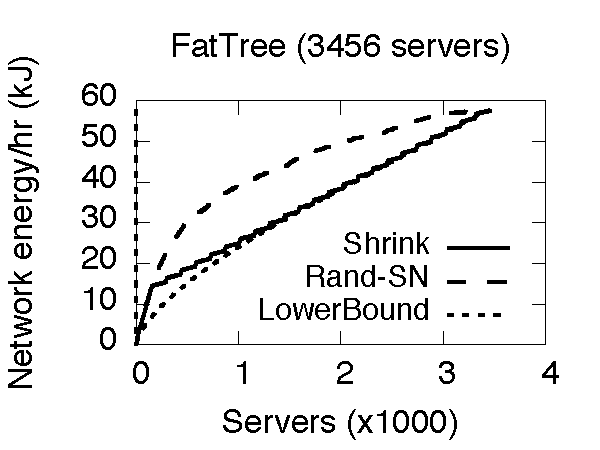
\includegraphics[scale=0.4]{graphs/final/fattree-24.pdf}
                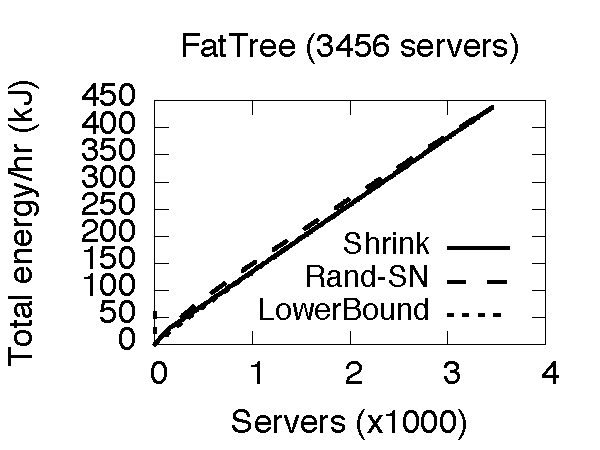
\includegraphics[scale=0.4]{graphs/final/fattree-24-total.pdf}
                        \centering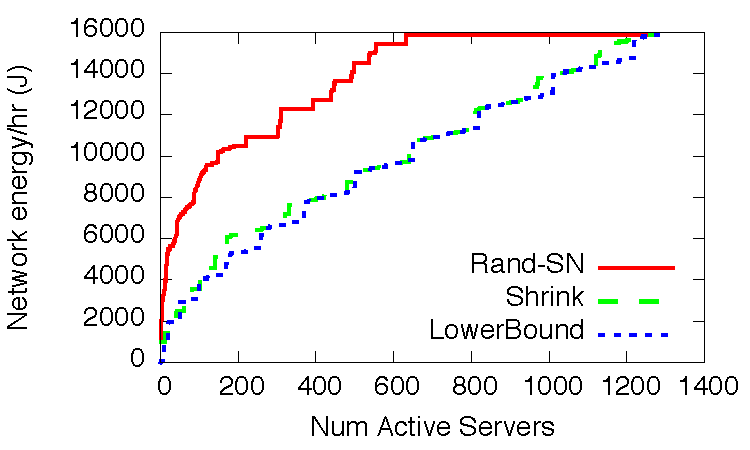
\includegraphics[scale=0.4]{graphs/final/vl2.pdf}
                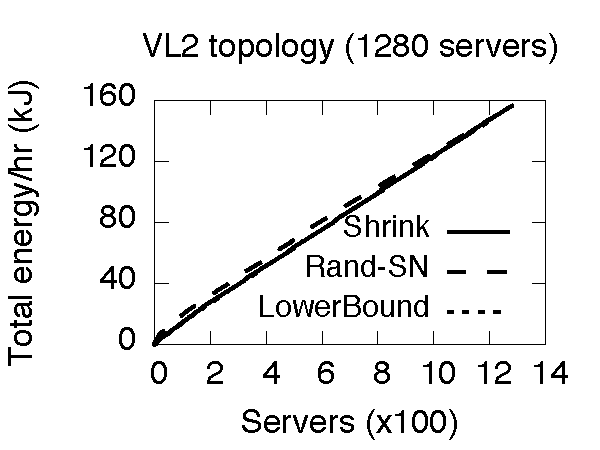
\includegraphics[scale=0.4]{graphs/final/vl2-total.pdf}
\caption{[Numerical computation] \shrink's network energy use is lower than a network-unaware server consolidation scheme \randSN\ by 38\% on FatTree and 42\% on VL2 when one-fourth of the servers are active in each topology.}
\label{fig:fattree}
\end{figure}

\subsection{Comparing network energy use}
\label{sec:net-compare}

\textbf{Schemes compared:}   (1) \emph{\randSN:} \randSN\ selects the set of active servers randomly; it uses the same network consolidation scheme as \shrink.  \randSN\ is used to evaluate the benefit of network-aware server consolidation in \shrink. (2) \emph{LowerBound:} We define lower bounds on the network energy use for a given number of active servers on the FatTree and the VL2 topologies. Our computation of LowerBound for FatTree and VL2 is described in Appendix \ref{sec:netlb}. \randSN\ and LowerBound provide the same per-server bandwidth guarantee to external hosts as \shrink\ does.

\textbf{Topologies:}  We simulate two network topologies:  a 3456-server FatTree topology made of 24-port switches (Cisco Nexus 2224P, 80 Watt, 720 count) \cite{cisco-dc-switches} consuming 80 Watt per switch, and a 1280-server VL2 topology made of 24-port ToR switches (Cisco Nexus 2224P, 80 W, 64 count) \cite{cisco-dc-switches} and 16-port 10 Gigabit core or aggregation switches (Cisco Catalyst 6500, 480 W, 24 count) \cite{catalyst-6500}. We assume all active servers have identical power use (Acer Altos T350 F2, 130W at 60\% utilization \cite{spec}).

\textbf{Results:}  Figure \ref{fig:fattree} presents our results.
%compares \shrink\ against \randSN\ and the lower bounds on network energy use for the simulated topologies.
The relative difference between \shrink\ and \randSN\ reduces as the number of active servers increases. 
When 25\% and 50\% of servers are active, \shrink's network energy use is lower than \randSN\ by 38\% and 26\% respectively on FatTree and 42\% and 35\% respectively on VL2. 
When 25\% and 50\% of servers are active, \shrink's network energy use higher than LowerBound by 9\% and 2\% respectively on FatTree and by 13\% and 7\% respectively on VL2. 
These findings show that \shrink's network-aware server consolidation reduces the network energy use over network-unaware server consolidation schemes and gives network energy savings close to the lower bound.
When 25\% and 50\% of servers are active, \shrink's \emph{total} energy use is lower than \randSN\ by 9\% and 5\% respectively on FatTree and 10\% and 7\% respectively on VL2. 
Thus, \shrink's network-aware server consolidation is effective in reducing aggregate \cdc\ energy use as well. 

%Considering scenarios where at least one-fifth of servers are active, \shrink\ uses up to 39\% less network energy on FatTree and up to 45\% less energy on VL2 compared to the network-unaware scheme, \randSN. 


\begin{figure*}
        \centering
        \subfigure[Mean]{\label{fig:pe-mean}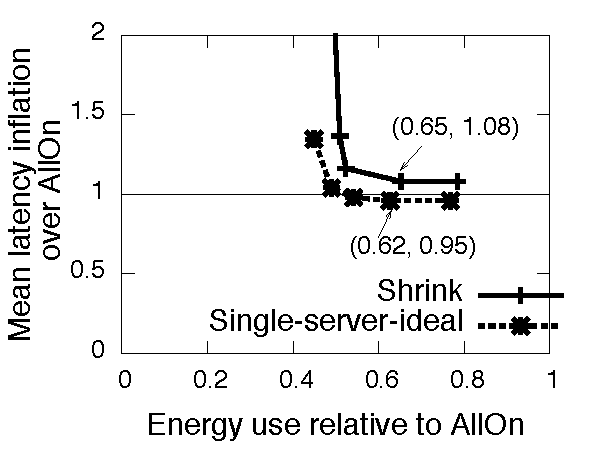
\includegraphics[scale=0.47]{graphs/final/mean.pdf}}
         \subfigure[95-th percentile]{\label{fig:pe-95}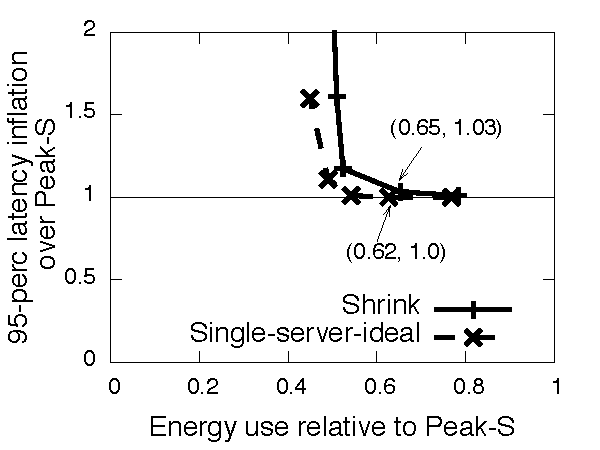
\includegraphics[scale=0.47]{graphs/final/perc95.pdf}}	       \subfigure[99-th percentile]{\label{fig:pe-99}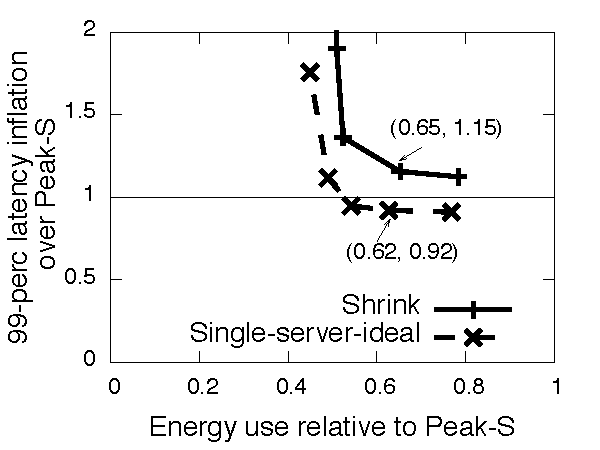
\includegraphics[scale=0.47]{graphs/final/perc99.pdf}}	
        \caption{Server consolidation (Section \ref{sec:ec2}):  \shrink's reduces energy over \peakS\ with a small response time inflation. In Figure \ref{fig:pe-mean}, \shrink's energy use is 0.65$\times$ of \peakS\ and its mean response time is 1.08$\times$ of \peakS; Single-server-ideal's energy use is 0.62$\times$  of \peakS\ and its mean response time is 0.95$\times$ of \peakS.}
        \label{fig:pe}
\end{figure*}

\subsection{Quantifying energy-response time tradeoff}
\label{sec:quantify}
\vspace{-0.1in}
\subsubsection{Experiment setup}
\label{sec:setup}
\textbf{Akamai dataset:} Our evaluation uses content access traces from an Akamai datacenter. The traces include all requests received at a datacenter with 24 servers for a week in December 2013. We restricted our data collection to a small datacenter as we did not have the resources to experiment with traces from a significantly larger datacenter. Our anonymized traces include several major types of traffic observed in a CDN such as video, social media and other web traffic. Each anonymized log entry includes among other fields, the request timestamp, content URL, size of requested content, actual number of bytes sent and IP address of the user. Overall, the traces contain more than 2 billion requests generating nearly 200 TB of network traffic.

\textbf{Testbeds:} We use prototype-based experiments (on EC2 and Emulab) and trace-based experiments. Our experiment on EC2 evaluates the energy-response time tradeoff due to server-only consolidation. As we do not have control over network topology on EC2, we use Emulab to evaluate the response time inflation due to both server and network consolidation. Finally, we conduct larger-scale trace-based experiments on a simulator.






%\begin{figure}[t]
%        \centering
%        \begin{subfigure}{0.24\textwidth}
%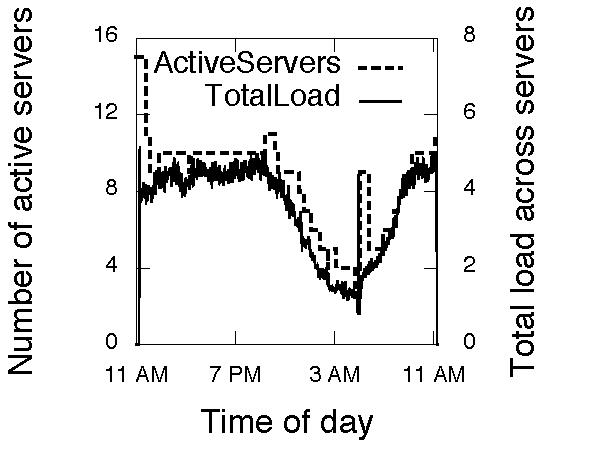
\includegraphics[scale=0.4]{graphs/final/num-servers.pdf}
%\caption{}
%\label{fig:num-servers}
%        \end{subfigure}
%        \begin{subfigure}{0.24\textwidth}
%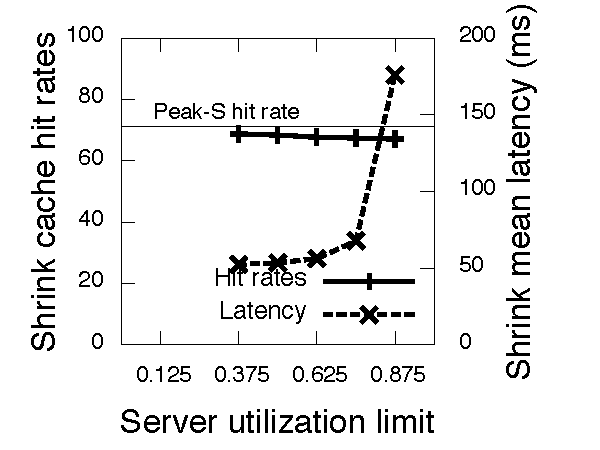
\includegraphics[scale=0.4]{graphs/final/hit-rate.pdf}
%\caption{}
%\label{fig:hitrate}
%        \end{subfigure}
%        \caption{[EC2] \shrink\ adapts the number of active servers based on \cdc\  load to reduce energy over \peakS. Cache hit rates and mean response time for \shrink\ and \peakS.}
%\end{figure}


%\centering
%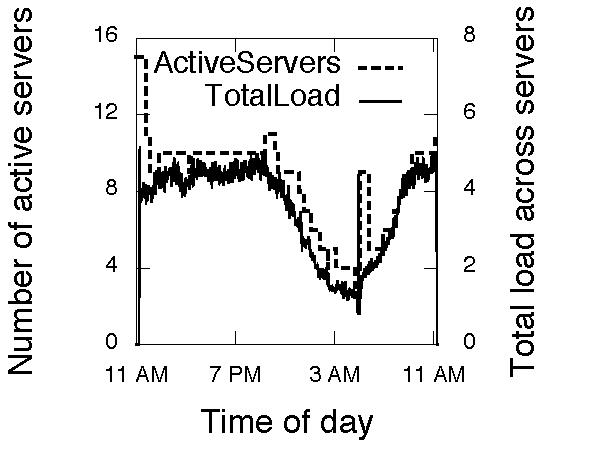
\includegraphics[scale=0.6]{graphs/final/num-servers.pdf}
%\caption{[EC2] \shrink\ adapts the number of active servers based on \cdc\  load to reduce energy over \peakS.}
%\label{fig:num-servers}
%\end{minipage}
%\hspace{0.5cm}
%\begin{minipage}{0.3\textwidth}
%\centering
%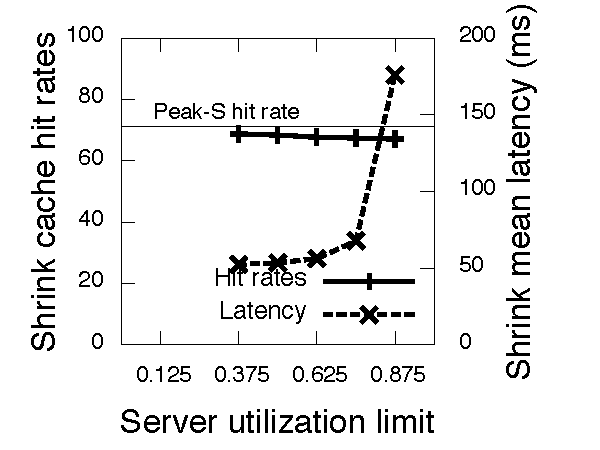
\includegraphics[scale=0.6]{graphs/final/hit-rate.pdf}
%\caption{[EC2] Cache hit rates and mean response time for \shrink\ and \peakS.}
%\label{fig:hitrate}
%\end{minipage}
%\hspace{0.5cm}
%\begin{minipage}{0.3\textwidth}
%\centering
%	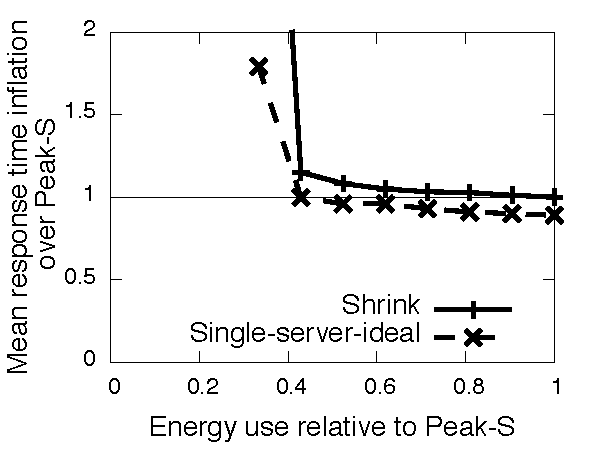
\includegraphics[scale=0.55]{graphs/final/emulab-mean.pdf}
%	\caption{[Emulab] Network and server consolidation: For an 15\% increase in mean response time, \shrink\ reduces energy use by 57\% over \peakS.}
%	\label{fig:pe-mean-2}
%
%\end{minipage}
%\end{figure*}

%
%\begin{figure*}
%\begin{minipage}{0.3\textwidth}
%\centering
%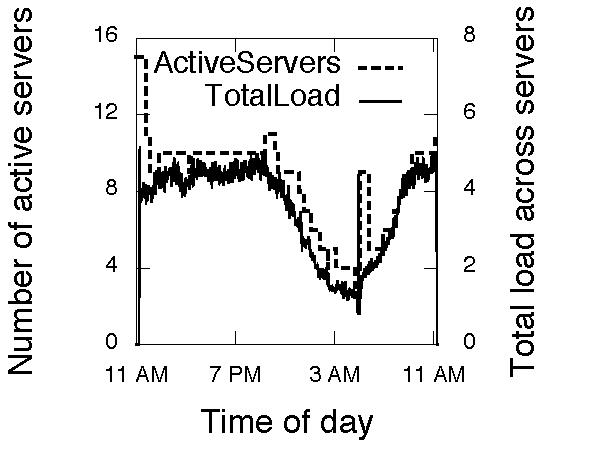
\includegraphics[scale=0.6]{graphs/final/num-servers.pdf}
%\caption{[EC2] \shrink\ adapts the number of active servers based on \cdc\  load to reduce energy over \peakS.}
%\label{fig:num-servers}
%\end{minipage}
%\hspace{0.5cm}
%\begin{minipage}{0.3\textwidth}
%\centering
%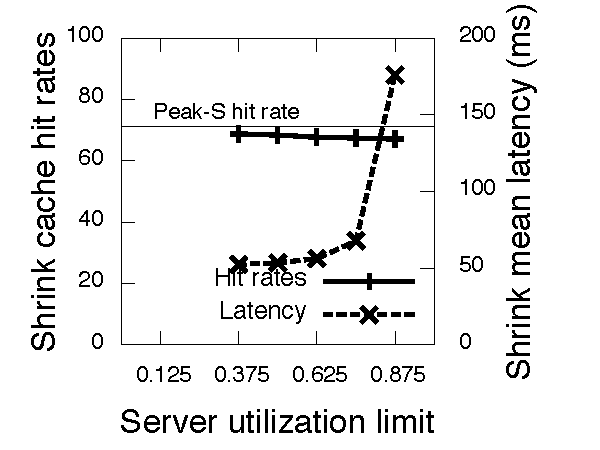
\includegraphics[scale=0.6]{graphs/final/hit-rate.pdf}
%\caption{[EC2] Cache hit rates and mean response time for \shrink\ and \peakS.}
%\label{fig:hitrate}
%\end{minipage}
%\hspace{0.5cm}
%\begin{minipage}{0.3\textwidth}
%\centering
%	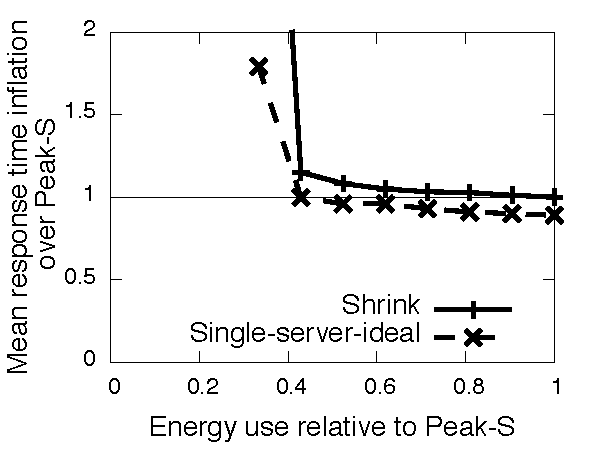
\includegraphics[scale=0.55]{graphs/final/emulab-mean.pdf}
%	\caption{[Emulab] Network and server consolidation: For an 15\% increase in mean response time, \shrink\ reduces energy use by 57\% over \peakS.}
%	\label{fig:pe-mean-2}
%
%\end{minipage}
%\end{figure*}


\textbf{Schemes compared:} We compare \shrink\ against \emph{\peakS} and \emph{Single-server-ideal}. \peakS\ represents a baseline in which a \cdc\ operator does not use consolidation to reduce energy use, i.e., it keeps all servers and switches active.

Single-server-ideal is a computation of the ideal energy-response time curve, unachievable by any real system. The points on this curve are obtained by varying the utilization $u$ up to which any server can be loaded. For a given $u$, the response time of Single-server-ideal for a given metric is equal to the measured load-vs.-response time curve of a single server for the same metric at the same utilization. For the same utilization $u$, any distributed system will have a higher response time because workload dynamics, load imbalance and non-steady state cache behavior; these factors are ignored by Single-server-ideal. Our single server measurements are done with a representative workload in the respective experimental environment, EC2 or Emulab, with emulated client-to-server delay and server-to-origin delay. 

%taken to be response of a single server in steady-state at the same utilization. In doing so, we assume that the response time of the entire \cdc\ at a given average utilization is the same as that of a single server  at the same utilization. 

For Single-server-ideal, we compute the set of servers and switches in each time interval that minimizes the total energy use as follows. Based on four inputs -- $u$, the total load in each time interval, the number of server transitions allowed, and the power model of each server --, we use a dynamic programming algorithm to compute the total energy use of servers and the number of active servers in each time interval. The number of transitions is equal to one on-off server transition/server/day or the same number of transitions as \shrink\ in that experiment, whichever is higher. The ideal network energy use for the tree topology we experiment with (Section \ref{sec:emulab}) is computed based on the number of active servers in each time interval. The set of active servers are selected in a left-to-right order; for each active server, we select the switches on the path to the root. The set of switches selected across all active servers is the set that optimizes network energy use.

%Single-server-ideal is a computation of the ideal energy-response time curve. In our computation, we assume that the utilization-vs.-response time curve for the entire \cdc\  is the same as that of a single server system at the same utilization, which is in steady state and has an infinite cache. 
%The response time of Single-server-ideal is \emph{ideal}, as discussed in Section \ref{sec:analysis}. For our computation, we obtained the utilization-vs.-response time curve for a single server by measuring response time metrics at varying request rates and using a cache size large enough so that steady state response times can be measured without exhausting the cache.
%
%The energy calculation for Single-server-ideal assumes prior knowledge of the total load in each time interval and the number of server transitions allowed. We allow Single-server-ideal to make one on-off server transition/server/day or the same number of transitions as \shrink\ in that experiment, whichever is higher. Based on these inputs, we use a dynamic programming algorithm \cite{mathew12} to compute the total energy use of servers and the number of active servers in each time interval.  The network energy use for the tree topology we experiment with (Section \ref{sec:emulab}) is computed as follows: For each active server, we select the switches on the path to the root. The set of switches selected across all active servers is the set that optimizes network energy use.



\subsubsection{Prototype-based experiments: server consolidation}
\label{sec:ec2}
\vspace{-0.1in}
This experiment quantifies the energy-response time tradeoff due to server consolidation on EC2. Our EC2 testbed consists of 15 servers, 15 clients and 4 origin servers running on independent m3.xlarge instances (4 core, 15 GB RAM, 40 GB$\times$2 SSD), all in the same datacenter. Our origin server is a trivial Apache Tomcat application that dynamically generates the requested content. We emulate a 60 ms RTT between origin servers and \cdc's servers, and a 10 ms RTT between client and server machines. We configured each server to use an 8 GB memory cache and a 30 GB cache on each SSD. 

Our workload consists of a 24-hour duration of the trace.  We selected one-eighth of the content randomly from the trace but sped up the trace by 8$\times$ to send those requests over a 3-hour duration. Thus, we  maintain approximately the same load on the servers. We use a short pre-shutdown wait interval $W =$ 10 min for \shrink\ because our workload is a sped up by $8\times$.

%
We calculate the energy savings relative to \peakS\ as per Equation \ref{eq:benefit}; the ratio of the idle to peak energy use of servers, $I$ equals 0.5 \cite{barroso2007case}. \peakS\ uses 15 servers in this experiment. We have conservatively chosen the number of servers in \peakS\ to be much less than the number of servers in the Akamai datacenter itself so as not to overestimate the energy savings. 



We evaluate \shrink\ in terms of three response time metrics --  mean, 95-percentile, 99-percentile. 
To provide a utilization-vs.-response time curve $F(.)$ to \shrink\ for each metric, we take the first approach discussed in Section \ref{sec:utilization-vs-responsetime}. The function $F(.)$ for each metric is equal to the measured utilization vs. response time curve of a single server with an inefficiency factor $\rho = 0.2$.  Based on $F(.)$ for each metric, we specify response times $F(u)$ to \shrink\ for values of $u$ from 0.375 to 0.875 at intervals of 0.125 across different runs. 

%, which is much less than the number of servers in the Akamai datacenter itself. we have made this choice not to overstate the energy savings.


Figure \ref{fig:pe} compares the response time and the energy use of \shrink\ relative to \peakS\ for the mean, the 95-th percentile and the 99-th percentile of response times. \shrink\ reduces energy use by 35\% over \peakS\ while inflating the mean, the 95-th percentile and the 99-th percentile by 8\%, 3\% and 15\% respectively. 
To explain the difference between \peakS\ and \shrink, consider Figure \ref{fig:ec2-other} (left)  which shows the aggregate load and the number of servers from one of the runs of the system. \shrink\  adapts the number of active servers based on load in the system keeping only 3 servers active when the load is the lowest, but \peakS\ always keeps 15 servers active and hence has a higher energy use. This result implies that an operator for which these inflations are tolerable, e.g., they do not cause an SLA violation, can achieve the corresponding energy savings as well. 




%Single-server-ideal does achieve a better energy-response time tradeoff than \shrink.  First, the energy-response time curve for Single-server-ideal is computed assuming that the response time for a given server utilization limit is equal to the response time of a single server in steady state at the same utilization. The response time for any real system, including \shrink, will be higher due to several reasons such as imperfect load balancing and non-steady state cache behavior. 




Does  an increase server load or a decrease in cache hit rates cause a greater impact on \shrink's response time over \peakS? 
In Figure \ref{fig:ec2-other} (right) the x-axis shows the server utilization limit $U$ computed by \shrink's consolidation algorithm (Section \ref{sec:serverconsolidation}) and y-axes show corresponding the  hit rates and the mean response time of \shrink. \shrink's  hit rates are lower than \peakS\ but the decrease is less than 7\% across all utilizations. 
Thus, the response time inflation due to a decrease in hit rates is likely to be small. A small reduction in hit rates is not surprising given that the Zipf exponent for the Akamai trace is 0.8 as per our calculations, and our model in Section \ref{sec:analysis} has suggested that  consolidation reduces hit rates by a small fraction for for real workloads with a high skew in content popularity.  We find that mean response times increase sharply at  a high server utilization limit, e.g. $U=0.875$, which is likely due to an increase in server load. To summarize, there is a small response time inflation due to a decrease in hit rates but severe inflation occurs at high server utilization limits, and is likely due to an increase in server  load.


Comparing \shrink\ with Single-server-ideal, in Figure \ref{fig:pe-mean}, \shrink's energy use is 0.65$\times$ of \peakS\ and its mean response time is 1.08$\times$ of \peakS; Single-server-ideal's energy use is 0.62$\times$  of \peakS\ and its mean response time is 0.95$\times$ of \peakS.  
There are two reasons that explain the gap between \shrink\ and Single-server-ideal. First, Single-server-ideal ignores several factors that increase response time of any distributed system such as workload dynamics, load imbalance and non-steady state cache behavior. Second, \shrink\ waits for the pre-shutdown wait interval to see if a decrease in load persists before turning servers off. But, in our calculation, Single-server-ideal knows the load for the entire experiment beforehand and hence it can shutdown servers sooner than \shrink\ and save more energy.

%An implication of our findings is that a simple random load balancing policy effectively avoids load hotspots and ensures only a small decrease in cache hit rates even as energy optimization schemes vary the number of active servers in a \cdc.
\begin{figure}
\centering
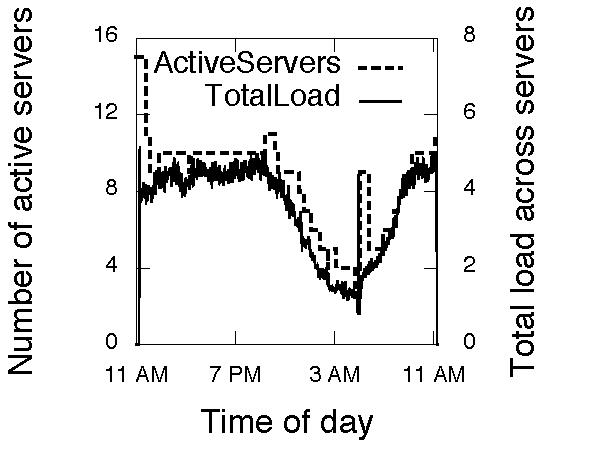
\includegraphics[scale=0.4]{graphs/final/num-servers.pdf}
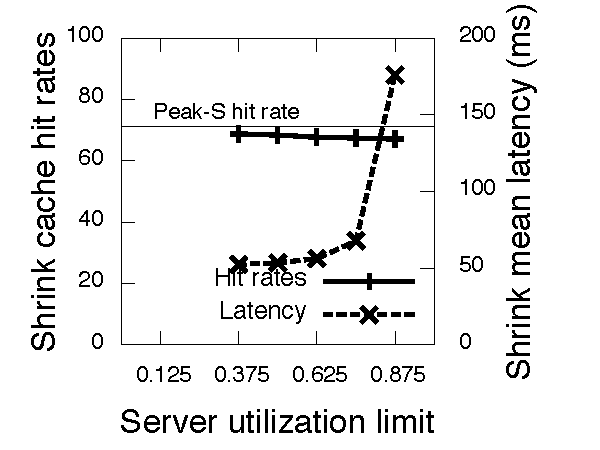
\includegraphics[scale=0.4]{graphs/final/hit-rate.pdf}
\caption{Server consolidation (Section \ref{sec:ec2}): [Left] \shrink\ adapts the number of active servers based on \cdc\  load to reduce energy over \peakS. [Right] Cache hit rates and mean response time for \shrink\ and \peakS.}
\label{fig:ec2-other}
\end{figure}

\subsubsection{Prototype-based experiments: server \& network consolidation}
\label{sec:emulab}

\begin{figure}
	\centering
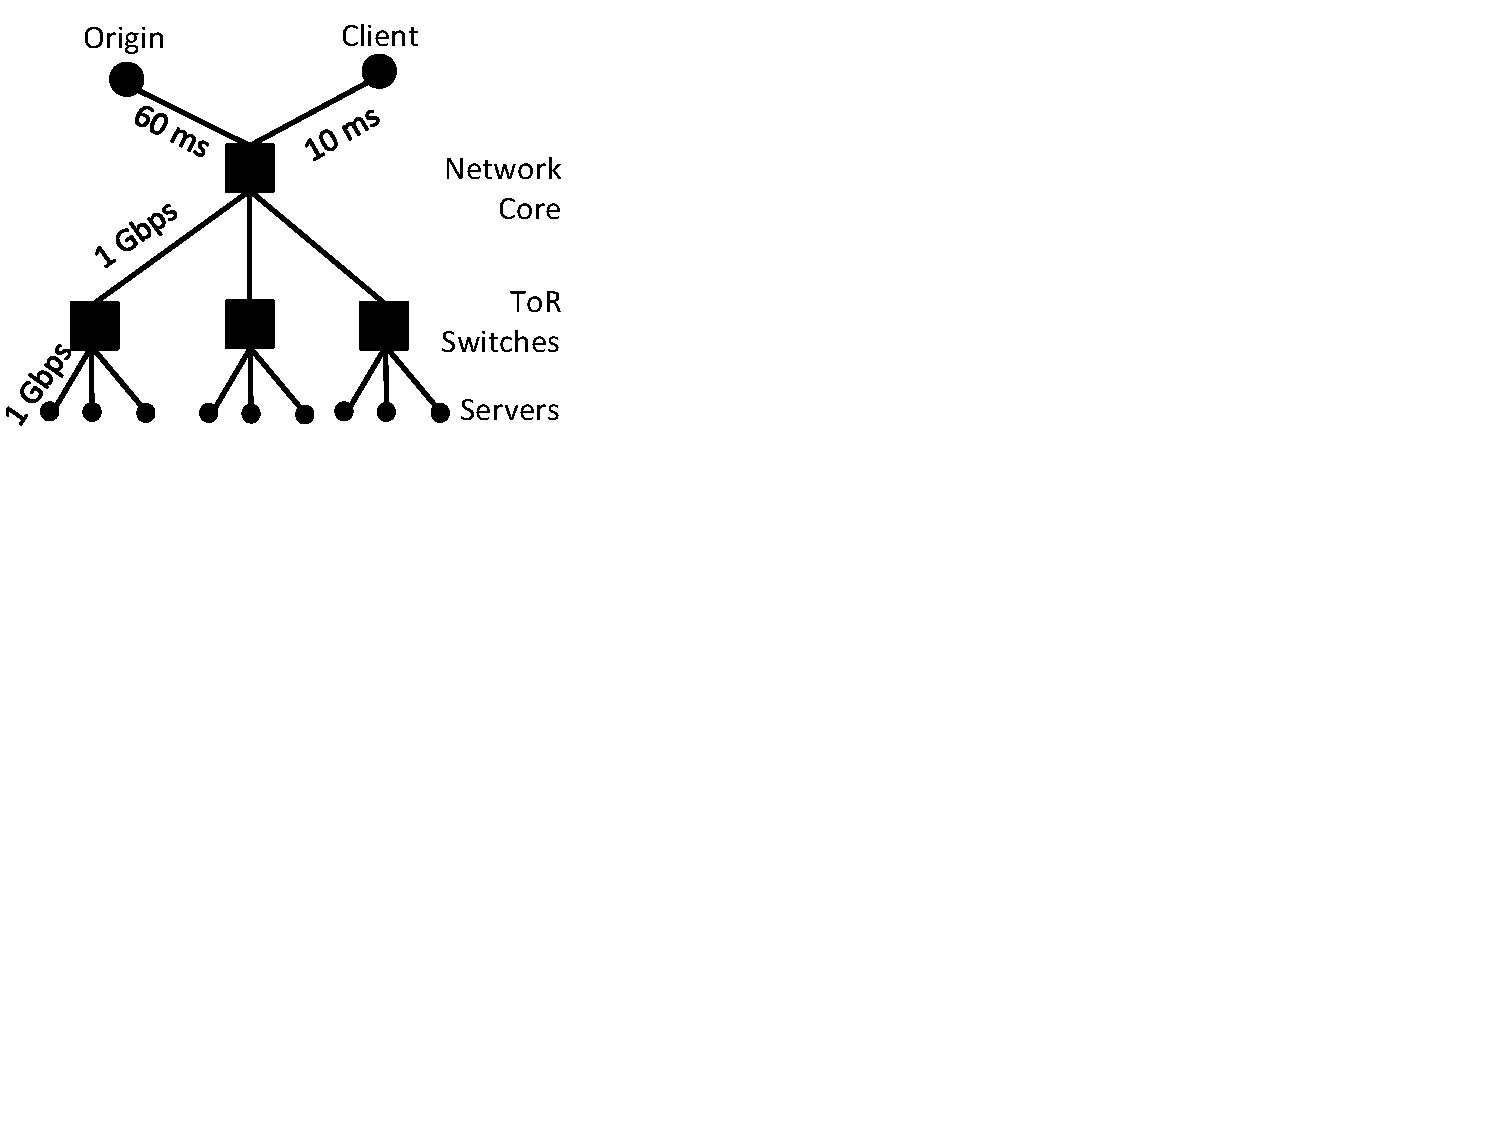
\includegraphics[scale=0.35]{figures/emulab-topo.pdf}
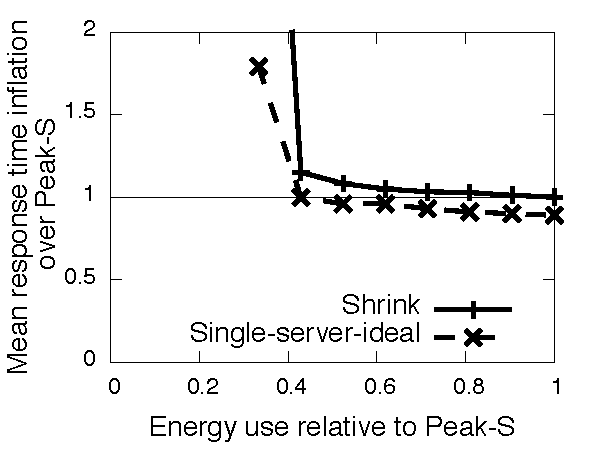
\includegraphics[scale=0.5]{graphs/final/emulab-mean.pdf}
\caption{Network and server consolidation (Section \ref{sec:emulab}): [Left] Emulab topology for the experiment. [Right] Compared to \peakS, \shrink\ has a 15\% higher response time but a 57\% lower energy use.}
\label{fig:emulab}
\end{figure}

We use Emulab to evaluate the energy-response time tradeoff when both server and network consolidation are being performed. For our experiment, we configure a tree topology with 1 Gbps links as shown in Figure \ref{fig:emulab} (left). 
In this topology, the ToR switches have 4 ports, and the core switch has at least 4 ports. Accordingly,  we calculate energy use of switches based on the power use of 4-port switch (Netgear GS105), which is 14.4 W \cite{netgearGS105}. The energy use of servers is computed using the same function as in the previous experiment. Our workload consists of a 1-hour duration of the trace containing requests for one-eighth of the content selected randomly.

Figure \ref{fig:emulab} (right) compares schemes in terms of the mean response times.  Across different runs that vary specified mean response times, \shrink\ uses between 2 and 9 servers; \peakS\ uses 9 servers.  We discuss the case when \shrink\ uses 3 servers so that only one of the ToR switches are being used as a result of network consolidation. In this case, the peak utilization of the link between the ToR and the core switch increased up to 76\% during the experiment, which is nearly three times higher than the peak link utilization for \peakS. Despite this increase, \shrink's response time is only 15\% higher than \peakS, while its network energy use is 50\% lower and the overall energy use is 57\% lower than \peakS\ (second point from the left in Figure \ref{fig:emulab} (right)). This result shows that both network and server consolidation can be performed with a small performance impact in \cdc s. Finally, we note that the difference between Single-server-ideal and \shrink\ is consistent with the difference between them in our experiment with server-only consolidation,, e.g., for the same energy savings as \shrink\ (= 57\%), \shrink's response time is 15\% more than Single-server-ideal.



%\begin{figure*}
%\begin{minipage}{0.3\textwidth}
%\centering
%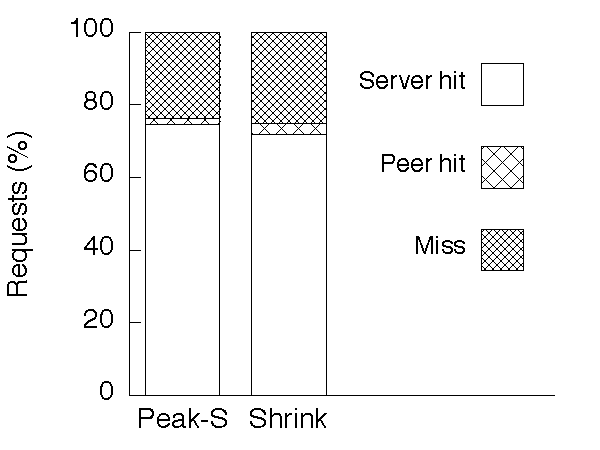
\includegraphics[scale=0.5]{graphs/final/sim-hitrate.pdf}
%\caption{[Simulator] \shrink\ increases miss rates by 1.5\% over \peakS\ over a one-week long trace showing that energy optimization in \cdc s hurts cache hit rates by a small margin. }
%\label{fig:sim-hitrate}
%\end{minipage}
%\hspace{0.5cm}
%\begin{minipage}{0.3\textwidth}
%\centering
%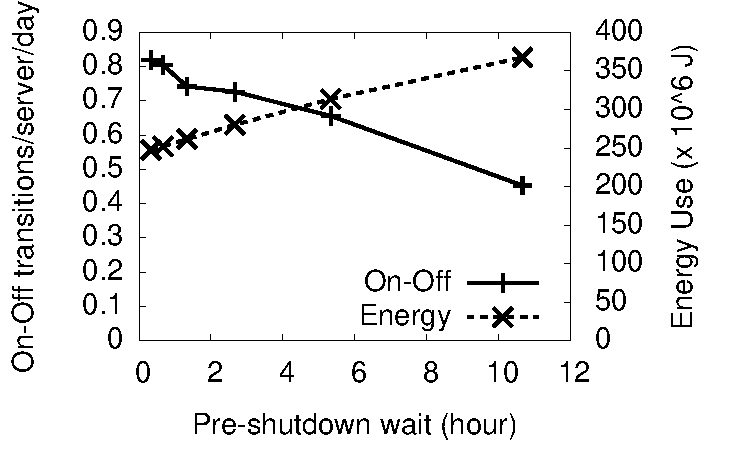
\includegraphics[scale=0.5]{graphs/final/onoff.pdf}
%\caption{[Simulator] Pre-shutdown wait interval ($W$) between 30 min \& 1 hour keeps on-off transition rate close to 1/server/day and with only a small increase in energy use over $W$ = 1 min.}
%\label{fig:sim-onoffrate}
%\end{minipage}
%\hspace{0.5cm}
%\begin{minipage}{0.3\textwidth}
%\centering
%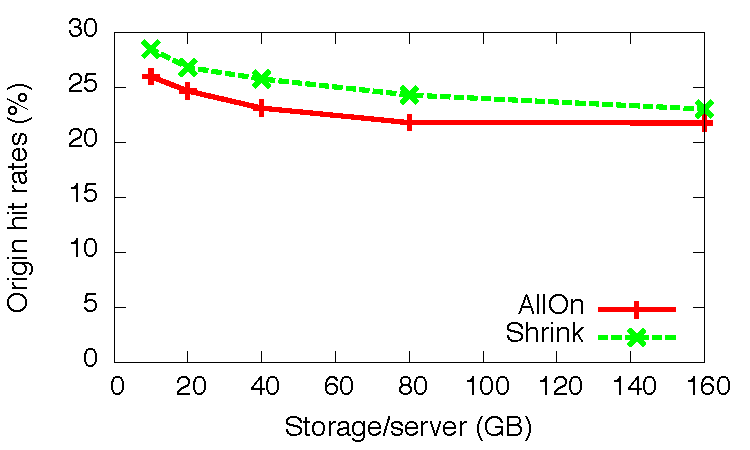
\includegraphics[scale=0.5]{graphs/final/storage.pdf}
%\caption{[Simulator] Difference between miss rates for both \shrink\ and \peakS\ is consistent despite variations in storage capacity.}
%\label{fig:sim-storage-vs-hitrate}
%\end{minipage}
%\end{figure*}

\subsubsection{Trace-based experiments}
\label{sec:simulation}
%The following are the goals of our trace-based experiments: (1) Quantify energy savings of server consolidation over the complete duration of the trace for a given server utilization limit expected to cause a small impact in response time.
%(2) Evaluate the potential benefit of cooperative caching among servers in a \cdc\ assuming that a cache-coordination protocol with a much smaller overhead can be developed in future. 
%(3) Quantify the tradeoff between energy savings and reliability by varying the pre-shutdown wait interval $W$.
%(4) Analyze the sensitivity of hit rates to a server's storage capacity.

\textbf{Methodology:} We conduct experiments for a \cdc\ with 16 servers for the week-long Akamai trace. The capacity of each server is defined in terms of network traffic it can support. The rate of network traffic generated by a request is a constant equal to the client bandwidth reported in the Akamai trace. To be able to fit the simulator process in the memory on our machine (32 GB), we filtered requests for one-eighth of the content from the trace. Accordingly, we scale down  the capacity of each server to be 150 Mbps, and the cache size per server to be 150 GB. Since trace-based experiments do not provide an accurate estimate of response times, we used a fixed server utilization limit $U$ = 0.65 for our experiments, which is expected to cause a small response time inflation (Figure \ref{fig:ec2-other} (right)). 
The cache hit rates of our simulator's LRU caching and Squid differ by less than 2\% for the same workload and cache size. 


\begin{figure}
\centering
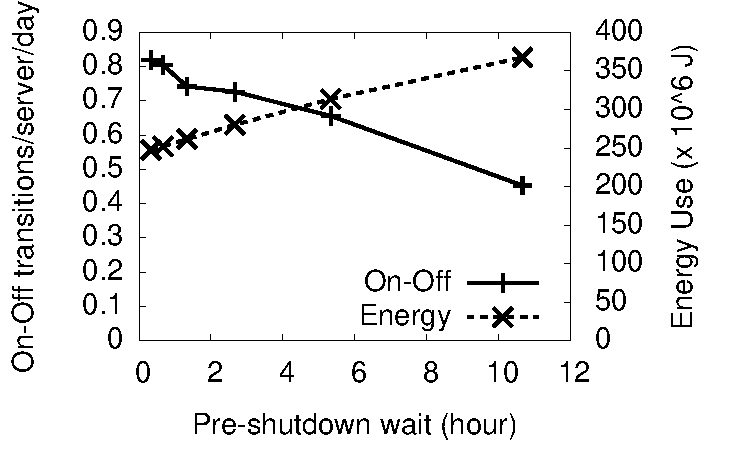
\includegraphics[scale=0.4]{graphs/final/onoff.pdf}
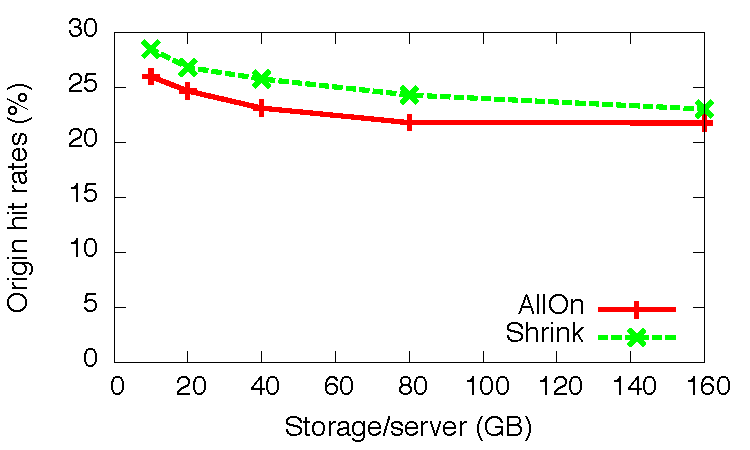
\includegraphics[scale=0.4]{graphs/final/storage.pdf}
\caption{[Simulator] [Left] Pre-shutdown wait interval between 30 min \& 1 hour keeps on-off transition rate close to 1/server/day. [Right] Comparison of miss rates for varying amounts of storage.}
\label{fig:sim-onoffrate}
\end{figure}
\textbf{Impact on hardware reliability:} Figure \ref{fig:sim-onoffrate} (left) shows the rate of on-off transitions per server and the corresponding energy savings is achievable. We find that a short pre-shutdown wait interval $W$ = 1 min hurts hardware reliability by increasing the rate of server transitions to more than 20/server/day. On the other hand, a  high $W$ = 4 hours reduces server transition rate to 0.81/server/day, but increases energy use by nearly 45\% over $W$ = 1 min.  The sweet spot for pre-shutdown wait interval is between 30 min to 1 hour, where increase in energy use over $W$ = 1 min is between 12\% and 15\%  but most of the reduction in on-off transition rates can still be achieved.

\textbf{Storage vs. cache miss rates:} To determine the sensitivity of miss rates to available storage, we evaluate \peakS\  and \shrink\ for varying amount of storage from 10 GB/server to 160 GB/server and present results in Figure \ref{fig:sim-onoffrate} (right). We remark that we have scaled down the CDN trace and hence the storage by a 8$\times$ factor, i.e., we would have provisioned 1.28 TB storage instead of 160 GB if we were to experiment with the full trace.  As storage reduces, the miss rates increase as expected. But, the relative difference between miss rates for both \shrink\ and \peakS\  remains nearly the same even on reducing the storage to 10 GB, e.g., \shrink's miss rates are 10.3\% higher than that of \peakS\  for 160 GB storage and are 9.6\% higher than that of \peakS\  for 10 GB storage. Thus, we conclude that server consolidation schemes are expected to increase datacenter miss rates by a small fraction within the range of storage typically available on server-class machines. 

\textbf{Cooperative caching benefit:} We evaluate the potential benefit of cooperative caching among servers in a \cdc\ assuming that a cache-coordination protocol with a much smaller overhead can be developed in future. The hit rates at cache peers  are 1.65\% for \peakS\  and 3.02\% for \shrink, which suggests that cooperative caching among datacenter servers, if implemented efficiently, could reduce the impact of energy optimization schemes by a small margin. 
%We present other results from trace-based experiments here. 
%(1) Over a one-week long trace. \shrink\ provides 37\% energy savings over \peakS. (2) 

%\textbf{Energy savings and cache hit rates:}
%We have compared the energy use of \shrink\ against other schemes over a one-week long trace. \shrink\ provides 37\% energy savings over \peakS\ in that experiment. We skip a detailed discussion of the results noting that energy use of other schemes are qualitatively similar to that observed in the experiment on EC2.
%
%Figure \ref{fig:sim-hitrate} compares the server hit rates, peer hit rates and miss rates. We make two key observations from this graph. First, there is less than 1.5\% difference in miss rates between \shrink\ and \peakS\  scheme, which supports our earlier observation in prototype-based experiments that \shrink's energy optimization does cause a significant increase in miss rates.  Second, we note that peer hit rates are 1.65\% for \peakS\  and 3.02\% for \shrink, which suggests that cooperative caching among datacenter servers could reduce the impact of energy optimization schemes by a small margin. Implementing a cooperative caching scheme with a low overhead is a topic of future work.




\eat{
%\begin{figure}
%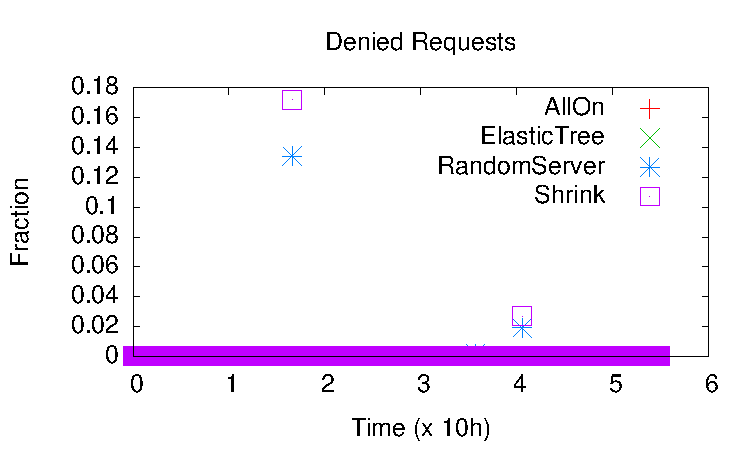
\includegraphics[scale=0.6]{graphs/server-logs/denied.pdf}
%\caption{Fraction of requests that are denied. \peakS\  scheme denies no requests throughout the experiment, whereas other schemes have a non-zero denied requests in a few time intervals. Both intervals  where requests are denied happened in cases of sudden spikes in load during night time.}
%\label{fig:sim-availability}
%\end{figure}

Figure \ref{fig:sim-availability} shows the fraction of requests that are denied due to server unavailability. Each data point represents denied requests in a 5-min interval. We find that the \peakS\  scheme has no denied requests throughout the experiment, i.e., it has 100\% availability. \shrink\ also has 100\% in all time intervals, except for two. Further analysis showed that both these intervals occured in late-night hours between 2 AM and 4 AM when there was unexpected spike in load that was 4 times the expected load in that interval. The active servers at that time did not sufficient enough resources to handle the request load. Thus, there was a brief period of unavailability until more servers could be turned on. That server unavailability is near-perfect an encouraging sign for deploying server consolidation, but also shows that energy-optimizing schemes make a \cdc\ less tolerant to highly unpredictable increase in load. A possible way to reduce the impact of such unavailability is to keep servers in a sleep state instead of completely turning them off so that they can be turned on quickly if necessary. 
}

%\begin{figure}
%\centering
%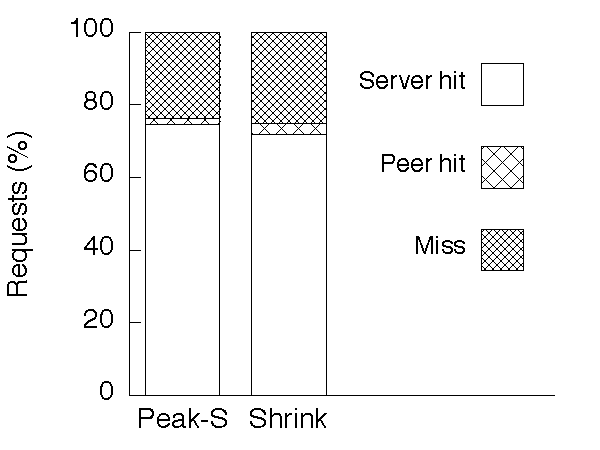
\includegraphics[scale=0.6]{graphs/final/sim-hitrate.pdf}
%\caption{[Simulator] \shrink\ increases miss rates by a small margin of 1.5\% over \peakS\ over a one-week long trace showing that energy optimization in \cdc s hurts cache performance by a small margin. }
%\label{fig:sim-hitrate}
%\end{figure}



%\begin{figure}
%\centering
%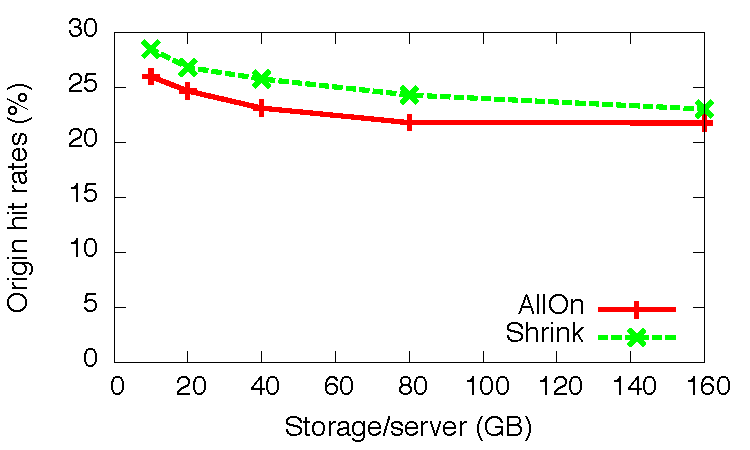
\includegraphics[scale=0.6]{graphs/final/storage.pdf}
%\caption{}
%\label{fig:sim-storage-vs-hitrate}
%\end{figure}




%!TEX root = shrink.tex

\section{Discussion}
\label{sec:discussion}

\textbf{Energy use vs. energy cost:} There are three types of \cdc s in terms of their energy cost to an operator. 

\emph{(1) Operator-owned facility:} If a \cdc\ operator owns the datacenter facility, it directly pays to the electricity companies based on its usage. In such datacenters, a reduction in energy use by \shrink\ is likely to bring a reduction in electricity costs as well.

\emph{(2) Co-location facility:} A \cdc\ at a co-location facility typically pays by the provisioned power and not the electricity used \cite{qureshi2009cutting}. Therefore, a reduction in energy use will not bring cost savings to \cdc\ operator with the existing pricing models. However, it is possible a \cdc\ operator may use the reduced energy as a leverage for negotiating a cheaper pricing. 

\emph{(3) Co-location inside ISP networks:} A \cdc\ at a co-location facility maintained by an ISP often has a symbiotic relation with the ISP, where the \cdc\ caches content to reduce the inter-domain traffic for the ISP while an ISP provides co-location free of charge \cite{google-caching}. In such \cdc s, energy savings do not translate to cost savings to the \cdc\ operator.  Although, energy savings do benefit the ISP, who eventually pays for the electricity.

The type of usage-based energy pricing also determines the cost savings for an operator. Specifically, we distinguish between flat rate pricing and time-of-use pricing \cite{pge-website}. With a flat rate pricing, a given percentage reduction in the energy use results in the same percentage reduction in the energy cost. With a time-of-use pricing, the percentage reduction in the energy use and the energy cost may not be the same. For example, if the peak load on a \cdc\ coincides with the peak hour of electricity prices, the percentage reduction in the energy cost would be lower than the percentage reduction in the energy use.

%\textbf{\shrink\ as a dynamic provisioning tool:} \shrink\ can be used as a dynamic provisioning tool by an operator that is running a content delivery site on infrastructure rented from a cloud-computing platform such as Amazon EC2. In such a setting, the operator may use \shrink\ to dynamically provision the number of active servers in accordance with incoming request load. In such a setting, the operator may not be able to perform network consolidation, but it can run the server energy optimization and load balancing sub-systems of \shrink\ and dynamically provision the number of active servers in accordance with incoming request load.  While functioning as a dynamic provisioning tool, \shrink\ can help reduce infrastructure costs for the operator.

\textbf{Impact on web-page load time:} Our prototype-based experiments evaluate the response time for individual HTTP requests, and hence do not capture a key metric that is more relevant from an end-user's perspective: web-page load time. However, we expect the inflation in web-page load time to be lower than the inflation in response times given that computation in web browsers constitutes up to 35\% of the critical path of a web-page load time \cite{wprof}.



\section{Related work}

Our effort distinguishes from prior work in quantifying the energy-response time tradeoff  in \cdc s, presenting the design and implementation of a system to leverage this tradeoff and proposing a network-aware server consolidation scheme to reduce network energy use.  Prior work on reducing energy of datacenters can be divided into three topics: (1) power-proportionality of servers and switches.  (2) server and network consolidation in a datacenter and (3) global load balancing across datacenters.

\textbf{Power-proportional servers and switches:}  Several efforts have focused on reducing energy use of a server's sub-systems such as CPU \cite{dvfs}, disk \cite{lu1999adaptive}, and memory \cite{fan2001memory}. Similarly, Nedevschi et al. \cite{Nedevschi08} study power management for switches that support sleep states or several power/performance states similar to CPUs. Nonetheless, today's servers and switches are far from power-proportional. Mahadevan et al. show that networking equipment consumes 62\%-91\% of their peak energy in idle state \cite{mahadevan2009power} and servers consume 32\% to 42\% of maximum power at a small utilization of 10\% \cite{spec}. Until the ideal of power-proportionality is achieved, consolidation remains a promising approach to save energy.

\textbf{Server consolidation:} Given the long line of work in server consolidation, our work does not focus on saving more energy than the existing consolidation schemes, but instead on accurately quantifying the impact on response times of a simple consolidation scheme.
%Both analytical and experimental studies of server consolidation have been previously explored. 

%A long line of work has studied consolidation techniques to reduce datacenter energy, including efforts that are analytical in nature as well as implementation-based efforts. 

The analytical work in this area shares similar goals as us.  Lin et al. \cite{lin12} propose an algorithm for optimizing a cost metric that incorporates energy costs, on-off switching costs and cost of degradation in performance. Mathew et al. \cite{mathew12} propose an algorithm that balances energy use, reliability and availability of servers, which they evaluate based on load traces from Akamai datacenters. In comparison, our implementation-based approach enables us to accurately model the relation between server utilization and response time, impact of server consolidation on cache hit rates, and non-ideal load balancing, to accurately quantify the impact of consolidation on response time for \cdc s.

Several efforts have conducted an implementation-based evaluation of server consolidation for stateless systems. Chase et al. \cite{chase2001managing} allocate resources among multiple co-hosted services in a cluster while reducing energy via consolidation. Pinheiro's \cite{pinheiro2001load} system proposes consolidation and load balancing algorithms given a bound on the performance degradation that is acceptable.  Rajamani et al. \cite{rajamani2003evaluating} evaluate consolidation schemes for a modified TPC-W workload. In comparison, our effort focuses on \cdc s that maintain a large amount of state in the form of cached content. In \cdc s, the effect of consolidation on response times cannot be evaluated accurately without accounting for the effect of consolidation on the availability of cached content and the resulting cache hit rates.
%One of our key findings is that consolidation results in a small impact on cache hit rates, which helps \shrink\ achieve a good energy-response time tradeoff.

Trushkowsky et al. \cite{Trushkowsky:2011}  dynamically allocate servers and reconfigure the data stored on the servers to meet service-level objectives such as 99-th percentile request latency.  However, there are two key differences between their work and ours. First, they focus  on a workload exclusively of small (256B) objects stored in-memory, whereas  \cdc s need to deal with orders of magnitude of heterogeneity in object sizes and extensively use a disk cache to improve hit rates.  Second, their system appears to be a backend data store, which always has content available within the datacenter. In comparison, \cdc s have a significant fraction of traffic to remote datacenters due to cache misses, and the impact of consolidation on response time in \cdc s depends on the increase in traffic to remote datacenters that consolidation causes. For these reasons, it is not clear if their findings on the impact of dynamic server allocation on request latency would be applicable for \cdc s.
%One of our key findings is that consolidation results in a small increase in cache miss rates, which helps \shrink\ achieve a good energy-response time tradeoff. 

%\TBD{we optimize network energy use also}

\textbf{Network consolidation:} Network  consolidation has been studied for both wide-area and data center networks \cite{response, elasticTree, greenTE, Chiaraviglio, Andrews}. Network consolidation concentrates traffic, represented in the form of a traffic matrix, on a subset of links and switches, and turns off remaining switches and links to save energy. Our work differentiates from prior work in two ways. First, prior work evaluates schemes mostly using traffic engineering metrics such as link utilization, while we evaluate actual end user response time for a real application and show that network consolidation can be performed with a small performance impact in \cdc s. Second, we show network consolidation is closely related to server consolidation. Our network-aware server consolidation saves up to 45\% more network energy over a network-unaware server consolidation scheme.
%network-aware server consolidation increase the potential savings that a network consolidation scheme can achieve. 
%
%
%
%
%
%
% with little effort on measuring response times for real applications
%
%While previous work has studied server and network consolidation as independent problems, we show that these problems are closely related. For the same number of servers, which set of servers is chosen affects potential energy savings that a network consolidation scheme can achieve. Further, we propose a simple network-aware server consolidation scheme saves up to 45\% more network energy over a network-unaware server consolidation scheme.

\textbf{Global load balancing:} Many papers \cite{Liu11,qureshi2009cutting,Gao12,Rao10}  have shown that geographical load-balancing across data centers can exploit the differences in electricity prices and in renewable energy availability at various locations to reduce energy costs, energy use, or non-renewable energy use.  In comparison, our work focus on improving energy-efficiency of a single \cdc\ by the use of consolidation. We believe that global load balancing can complement \shrink\ in reducing energy use and its cost across datacenters.

%!TEX root = shrink.tex
\section{Conclusions}
Content datacenters used for storing and serving content to end-users are common today. A major barrier to  widespread adoption of server and network consolidation is \cdc\ operators' concern on the impact on SLAs or user-perceived latencies. Our work takes a step towards addressing this concern by presenting a model to quantify the energy savings vs. latency inflation trade-off in \cdc s.  A key insight, supported via experiments, is that despite server consolidation, cache hit rates remain close to an unconsolidated datacenter,  which helps mitigate the impact of consolidation on user-perceived latencies. We have designed and implemented \shrink, a system that leverages this tradeoff to yield significant energy savings while affecting user-perceived latencies in a controlled manner. \shrink's novel network-aware server consolidation algorithm reduces network energy use by up to 42\% compared to network-unaware server consolidation schemes. \shrink, in experiments based on content access traces from an Akamai datacenter, reduced energy use by 35\% compared to a baseline scheme that keeps entire datacenter always on while increasing mean latency by 8\% over it. Overall, our findings encourage deployment of consolidation techniques to reduce \cdc\ energy use.

\bibliographystyle{abbrv}
\bibliography{New}  % sigproc.bib is the name of the Bibliography in this case
% You must have a proper ".bib" file
%  and remember to run:
% latex bibtex latex latex
% to resolve all references
%
% ACM needs 'a single self-contained file'!
%
%APPENDICES are optional
\balancecolumns
%%!TEX root = shrink.tex

\section{Discussion}
\label{sec:discussion}

\textbf{Energy use vs. energy cost:} There are three types of \cdc s in terms of their energy cost to an operator. 

\emph{(1) Operator-owned facility:} If a \cdc\ operator owns the datacenter facility, it directly pays to the electricity companies based on its usage. In such datacenters, a reduction in energy use by \shrink\ is likely to bring a reduction in electricity costs as well.

\emph{(2) Co-location facility:} A \cdc\ at a co-location facility typically pays by the provisioned power and not the electricity used \cite{qureshi2009cutting}. Therefore, a reduction in energy use will not bring cost savings to \cdc\ operator with the existing pricing models. However, it is possible a \cdc\ operator may use the reduced energy as a leverage for negotiating a cheaper pricing. 

\emph{(3) Co-location inside ISP networks:} A \cdc\ at a co-location facility maintained by an ISP often has a symbiotic relation with the ISP, where the \cdc\ caches content to reduce the inter-domain traffic for the ISP while an ISP provides co-location free of charge \cite{google-caching}. In such \cdc s, energy savings do not translate to cost savings to the \cdc\ operator.  Although, energy savings do benefit the ISP, who eventually pays for the electricity.

The type of usage-based energy pricing also determines the cost savings for an operator. Specifically, we distinguish between flat rate pricing and time-of-use pricing \cite{pge-website}. With a flat rate pricing, a given percentage reduction in the energy use results in the same percentage reduction in the energy cost. With a time-of-use pricing, the percentage reduction in the energy use and the energy cost may not be the same. For example, if the peak load on a \cdc\ coincides with the peak hour of electricity prices, the percentage reduction in the energy cost would be lower than the percentage reduction in the energy use.

%\textbf{\shrink\ as a dynamic provisioning tool:} \shrink\ can be used as a dynamic provisioning tool by an operator that is running a content delivery site on infrastructure rented from a cloud-computing platform such as Amazon EC2. In such a setting, the operator may use \shrink\ to dynamically provision the number of active servers in accordance with incoming request load. In such a setting, the operator may not be able to perform network consolidation, but it can run the server energy optimization and load balancing sub-systems of \shrink\ and dynamically provision the number of active servers in accordance with incoming request load.  While functioning as a dynamic provisioning tool, \shrink\ can help reduce infrastructure costs for the operator.

\textbf{Impact on web-page load time:} Our prototype-based experiments evaluate the response time for individual HTTP requests, and hence do not capture a key metric that is more relevant from an end-user's perspective: web-page load time. However, we expect the inflation in web-page load time to be lower than the inflation in response times given that computation in web browsers constitutes up to 35\% of the critical path of a web-page load time \cite{wprof}.



\section{Related work}

Our effort distinguishes from prior work in quantifying the energy-response time tradeoff  in \cdc s, presenting the design and implementation of a system to leverage this tradeoff and proposing a network-aware server consolidation scheme to reduce network energy use.  Prior work on reducing energy of datacenters can be divided into three topics: (1) power-proportionality of servers and switches.  (2) server and network consolidation in a datacenter and (3) global load balancing across datacenters.

\textbf{Power-proportional servers and switches:}  Several efforts have focused on reducing energy use of a server's sub-systems such as CPU \cite{dvfs}, disk \cite{lu1999adaptive}, and memory \cite{fan2001memory}. Similarly, Nedevschi et al. \cite{Nedevschi08} study power management for switches that support sleep states or several power/performance states similar to CPUs. Nonetheless, today's servers and switches are far from power-proportional. Mahadevan et al. show that networking equipment consumes 62\%-91\% of their peak energy in idle state \cite{mahadevan2009power} and servers consume 32\% to 42\% of maximum power at a small utilization of 10\% \cite{spec}. Until the ideal of power-proportionality is achieved, consolidation remains a promising approach to save energy.

\textbf{Server consolidation:} Given the long line of work in server consolidation, our work does not focus on saving more energy than the existing consolidation schemes, but instead on accurately quantifying the impact on response times of a simple consolidation scheme.
%Both analytical and experimental studies of server consolidation have been previously explored. 

%A long line of work has studied consolidation techniques to reduce datacenter energy, including efforts that are analytical in nature as well as implementation-based efforts. 

The analytical work in this area shares similar goals as us.  Lin et al. \cite{lin12} propose an algorithm for optimizing a cost metric that incorporates energy costs, on-off switching costs and cost of degradation in performance. Mathew et al. \cite{mathew12} propose an algorithm that balances energy use, reliability and availability of servers, which they evaluate based on load traces from Akamai datacenters. In comparison, our implementation-based approach enables us to accurately model the relation between server utilization and response time, impact of server consolidation on cache hit rates, and non-ideal load balancing, to accurately quantify the impact of consolidation on response time for \cdc s.

Several efforts have conducted an implementation-based evaluation of server consolidation for stateless systems. Chase et al. \cite{chase2001managing} allocate resources among multiple co-hosted services in a cluster while reducing energy via consolidation. Pinheiro's \cite{pinheiro2001load} system proposes consolidation and load balancing algorithms given a bound on the performance degradation that is acceptable.  Rajamani et al. \cite{rajamani2003evaluating} evaluate consolidation schemes for a modified TPC-W workload. In comparison, our effort focuses on \cdc s that maintain a large amount of state in the form of cached content. In \cdc s, the effect of consolidation on response times cannot be evaluated accurately without accounting for the effect of consolidation on the availability of cached content and the resulting cache hit rates.
%One of our key findings is that consolidation results in a small impact on cache hit rates, which helps \shrink\ achieve a good energy-response time tradeoff.

Trushkowsky et al. \cite{Trushkowsky:2011}  dynamically allocate servers and reconfigure the data stored on the servers to meet service-level objectives such as 99-th percentile request latency.  However, there are two key differences between their work and ours. First, they focus  on a workload exclusively of small (256B) objects stored in-memory, whereas  \cdc s need to deal with orders of magnitude of heterogeneity in object sizes and extensively use a disk cache to improve hit rates.  Second, their system appears to be a backend data store, which always has content available within the datacenter. In comparison, \cdc s have a significant fraction of traffic to remote datacenters due to cache misses, and the impact of consolidation on response time in \cdc s depends on the increase in traffic to remote datacenters that consolidation causes. For these reasons, it is not clear if their findings on the impact of dynamic server allocation on request latency would be applicable for \cdc s.
%One of our key findings is that consolidation results in a small increase in cache miss rates, which helps \shrink\ achieve a good energy-response time tradeoff. 

%\TBD{we optimize network energy use also}

\textbf{Network consolidation:} Network  consolidation has been studied for both wide-area and data center networks \cite{response, elasticTree, greenTE, Chiaraviglio, Andrews}. Network consolidation concentrates traffic, represented in the form of a traffic matrix, on a subset of links and switches, and turns off remaining switches and links to save energy. Our work differentiates from prior work in two ways. First, prior work evaluates schemes mostly using traffic engineering metrics such as link utilization, while we evaluate actual end user response time for a real application and show that network consolidation can be performed with a small performance impact in \cdc s. Second, we show network consolidation is closely related to server consolidation. Our network-aware server consolidation saves up to 45\% more network energy over a network-unaware server consolidation scheme.
%network-aware server consolidation increase the potential savings that a network consolidation scheme can achieve. 
%
%
%
%
%
%
% with little effort on measuring response times for real applications
%
%While previous work has studied server and network consolidation as independent problems, we show that these problems are closely related. For the same number of servers, which set of servers is chosen affects potential energy savings that a network consolidation scheme can achieve. Further, we propose a simple network-aware server consolidation scheme saves up to 45\% more network energy over a network-unaware server consolidation scheme.

\textbf{Global load balancing:} Many papers \cite{Liu11,qureshi2009cutting,Gao12,Rao10}  have shown that geographical load-balancing across data centers can exploit the differences in electricity prices and in renewable energy availability at various locations to reduce energy costs, energy use, or non-renewable energy use.  In comparison, our work focus on improving energy-efficiency of a single \cdc\ by the use of consolidation. We believe that global load balancing can complement \shrink\ in reducing energy use and its cost across datacenters.

%Appendices



\chapter{Network energy lower bound}
\label{sec:netlb}
We derive lower bounds on the network energy use for FatTree \cite{fattree} and VL2 \cite{vl2} under the constraint that $n$  servers that are active must be able to simultaneously send traffic to clients equal to the external bandwidth $E$ via the set of active switches only.

\textbf{VL2:} Let the energy use of each core, aggregation and ToR switch be $PC$, $PA$ and $PT$ respectively.
Let $L$ be the capacity of links between each pair of core and aggregation switches. 
If  $c$ core switches and $a$ aggregation switches be active, then
the maximum number of servers that can be supported is $ \textit{nmax} = (a\times c\times L/E)$ and the total energy use of core and aggregation switches is $\textit{etotal} = (c \times PC + a \times PA)$. 
We select the optimal values of $\textit{a\_opt}$ and $\textit{c\_opt}$ (by enumerating all values) such that \textit{etotal} is minimized under the constraint that $\textit{nmax} > n$. 
Assuming each ToR switch connects to $k$ servers,  the minimum number of ToR switches needed is $\lceil n/k \rceil$. 
Thus, a lower bound on the total network energy use is $(\lceil n/k \rceil PT) + (\textit{c\_opt} \times PC + \textit{a\_opt} \times PA)$.


\textbf{FatTree:} Switches are identical in a FatTree. So, a lower bound the number of active switches gives a lower bound on network energy use also.




Let $m_1, \cdots m_k$ be the active servers in the $k$ pods so that $m_1 + \cdots + m_k = n$.  In a pod with $m$ active servers, at least $2 \sqrt{m}$ switches must be active. Thus, a total of $(2 (\sqrt{m_1} + \cdots + \sqrt{m_k} ))$ pod switches must be active. 

Let $c$ be the number of active core switches. We claim that the number of active servers in any pod can at most be $c$. The reason is that a core switch has only one link to switches in each pod, and hence can receive traffic from only one server sending traffic at its outgoing link capacity to external clients. The values of $m_1, \cdots m_k$ that minimizes the number of active pod switches is given by $m_1 = m_2 = \cdots = m_l = c$,  $m_{l+1} = (n \bmod c)$, and $m_{l+2} = m_{l+3} = \cdots  m_{k} = 0$, where $l = \lfloor n/c \rfloor$.  Let $p$ be minimum number of active pod switches thus computed. Then, the minimum number of total active switches active is given by $(p+c)$.



% If $m_1, \cdots m_k$ are the active servers in the $k$ pods, then a total of $(2 (\sqrt{m_1} + \cdots + \sqrt{m_k} ))$ pod switches must be active.


%If $c$ core switches are active, the values of $m_1, \cdots m_k$ where $m_1 + \cdots + m_k = n$ that minimizes the number of active pod switches is given by $m_1 = m_2 = \cdots = m_l = c$,  $m_{l+1} = (n \bmod c)$, and $m_{l+2} = m_{l+3} = \cdots  m_{k} = 0$, where $l = \lfloor n/c \rfloor$.  Let $p$ be minimum number of active pod switches thus computed. Then, the minimum number of total active switches active is given by $(p+c)$.

Computing the minimum number of switches for all possible values of $c\ (c \leq n, c \leq k^2/4)$ and taking their minimum gives a lower bound on the number of active switches for this topology.

%taking the least possible value of $c$ for which 



%\textbf{FatTree:} A $k$-FatTree is built using identical switches with $k$ ports of equal capacity. We compute the least number of core, upper-level pod and lower-level pod switches that are active. Each lower-level pod switch is connected to $k/2$ servers. Therefore, at least $\lceil n/(k/2) \rceil$ lower-level pod switches are active. Each upper-level pod switch has $k/2$ ports to lower-level pod switches and hence it can receive traffic from at most $k/2$ servers sending traffic at their outgoing link capacity to external clients. Thus, $\lceil n/(k/2) \rceil$ upper-level pod switches are active. Each core switch has only one link to switch in each pod, and hence can receive traffic from only one server sending traffic at its outgoing link capacity to external clients. Thus, the minimum number of core switches is equal to the maximum number of servers that are active in any pod. There at least one out of $k$ pods has at least $\lceil n/k \rceil$ active servers. In total, $(\lceil n/k \rceil + 2 \lceil n/(k/2) \rceil)$ switches must be active.

%Since each  lower-level pod switch and upper-level pod switch supports at most $k/2$ active servers, at least $\lceil n/(k/2) \rceil $ lower-level pod switches and upper-level pod switches must be active.



\eat{
\section{Characteristic time approx.}
\label{sec:approximation}
The characteristic-time approximation computes the hit rates of each content served by an LRU cache \cite{che2002hierarchical}. This approximation has proved accurate for workloads with a Zipf content popularity distribution.  Let $O$ be the set of unit-sized content served by a cache of size $S$ units and $l_j$ denote the request rate for content $j \in O$. Solving the equations below using fixed-point approximation yields the hit rates, $h_j$, for content $j \in O$ and, $T$, the characteristic time of the cache. The cache hit rate across all content is $\frac{\sum_{j\in O}h_j l_j}{\sum_{j\in O} l_j}$. 
\[h_i = 1 - e^{l_j T}\quad \forall j \in O\]
\[\sum_{j \in O} h_j = S \]
}

\eat{
\section{MIP for energy optimal node selection}
\label{sec:optimal}

We describe the optimal strategy for selecting servers and switches that minimize network energy use given the number of active servers in a datacenter and the traffic flow from each active server to the client node. Let $N$ be the set of all nodes in a 3-level datacenter topology, with servers $S$ as leaves  and switches $R$, and a virtual client node $c$. We assume a tree-like datacenter topology in which all links are between nodes with a difference of one in their heights. The virtual client node is the root node in the topology is connected via infinite capacity links to all core-switches. Let $E$ be the set of unidirectional edges in the datacenter in the direction from leaves to root, such that $e_{ij}$ is the link from node $i\in N$ to node $j \in N$ with link capacity $C_{ij}$. Let $O(j)$ and $I(j)$ are incoming and outgoing links at switch $j$. 
 Let $f$ be the traffic flow from each active server to the client node. Further, the number of servers to be kept active is $A$. Switch $i \in R$ consumes power $P_i$ and the power use of ports at the two ends of link $e_{ij}$ $Q_{ij}$  and $Q_{ji}$.  Let $s_i$ denote a binary variable indicating whether server $i \in S$ is turned on. Let $r_i$ denote a binary variable indicating whether switch $i \in R$ is turned on. Let, $t_{ij}$ denote a  binary variable indicating whether link $e_{ij} \in E$ is active.


\[\textit{Minimize:}\quad\sum_{i \in R} r_i P_i+\sum_{e_{ij} \in E} t_{ij} (Q_{ij} + Q_{ji})\]

\emph{Constraints:}

\[\sum_{i \in R} s_i = A \quad\textit{\small{\# Number of active servers is A}}\]
\[f_{ij} = s_i f\ \ \forall i \in S, j \in \textit{O(i)}\ \  \textit{\small{\# Active server sends f traffic units}}\]
\[\sum_{e_{ij} \in O(j)}f_{ij}=\sum_{e_{jk} \in I(j)} f_{jk}\ \forall j \in R \ \textit{\small{\# Flow conservation at switch}}\]
\[f_{ij} \leq C_{ij} t_{ij} \ \forall e_{ij} \in E\ \textit{\small{\# Link, if on, carries traffic up to capacity}}\]
\[t_{ij} \leq r_j \  \forall j \in R, e_{ij} \in I(j)\ \textit{\small{\# Incoming links off, if switch is off}}\]
\[t_{jk} \leq r_j \  \forall j \in R, e_{jk} \in O(j)\ \textit{\small{\# Outgoing links off, if switch is off}}\]
\[r_j \leq \sum_{e_{ij} \in I(j) } t_{ij} \ \textit{\small{\# If all incoming links are active, switch is off}}\]
%\[r_j \leq \sum_{e_{jk} \in  O(j) } t_{jk}\ \textit{\# } \]
%\[s_i, r_k,  = \{0,1\} \forall i \in S, r_i = \{0,1\} \forall i \in R, t_{ij} = \{0,1\} \forall e_{ij} \in E\]

}

%%Appendix A
%\section{Headings in Appendices}
%The rules about hierarchical headings discussed above for
%the body of the article are different in the appendices.
%In the \textbf{appendix} environment, the command
%\textbf{section} is used to
%indicate the start of each Appendix, with alphabetic order
%designation (i.e. the first is A, the second B, etc.) and
%a title (if you include one).  So, if you need
%hierarchical structure
%\textit{within} an Appendix, start with \textbf{subsection} as the
%highest level. Here is an outline of the body of this
%document in Appendix-appropriate form:
%\subsection{Introduction}
%\subsection{The Body of the Paper}
%\subsubsection{Type Changes and  Special Characters}
%\subsubsection{Math Equations}
%\paragraph{Inline (In-text) Equations}
%\paragraph{Display Equations}
%\subsubsection{Citations}
%\subsubsection{Tables}
%\subsubsection{Figures}
%\subsubsection{Theorem-like Constructs}
%\subsubsection*{A Caveat for the \TeX\ Expert}
%\subsection{Conclusions}
%\subsection{Acknowledgments}
%\subsection{Additional Authors}
%This section is inserted by \LaTeX; you do not insert it.
%You just add the names and information in the
%\texttt{{\char'134}additionalauthors} command at the start
%of the document.
%\subsection{References}
%Generated by bibtex from your ~.bib file.  Run latex,
%then bibtex, then latex twice (to resolve references)
%to create the ~.bbl file.  Insert that ~.bbl file into
%the .tex source file and comment out
%the command \texttt{{\char'134}thebibliography}.
%% This next section command marks the start of
%% Appendix B, and does not continue the present hierarchy
%\section{More Help for the Hardy}
%The sig-alternate.cls file itself is chock-full of succinct
%and helpful comments.  If you consider yourself a moderately
%experienced to expert user of \LaTeX, you may find reading
%it useful but please remember not to change it.
%%\balancecolumns % GM June 2007
% That's all folks!
\end{document}

%
%
%\begin{document}
%
%\maketitle
%
%\section{Introduction}
%
%Raises energy concerns of content delivery systems. 
%
%States why prior work is incomplete: performance impact, e.g., cache misses and, no network energy minimization.
%
%\section{Motivation}
%
%
%
%\subsection{Joint optimization of network and server energy}
%
%\subsection{Performance Impact of Energy Savings}
%
%\subsubsection{Increase in server load}
%
%\subsubsection{Increase in user-perceived latency}
%
%\section{Energy minimizing strategies}
%
%\subsection{Cluster model}
%
%\subsection{Optimal strategy}
%
%\subsection{Heuristics}
%
%\subsection{Cross-cluster optimization}
%
%\section{Content Workload Analysis}
%
%\subsection{Datasets}
%
%\subsection{Predictability}
%
%\subsection{Locality}
%
%
%\section{Evaluation}
%
%%\subsection{Network energy savings potential}
%
%\subsection{Energy savings under normal operation}
%
%\subsection{Cross-cluster}
%
%\subsection{Fault-tolerance}
%
%\section{Implementation Outline}
%
%%!TEX root = Main.tex
\vsp
\section{Introduction}
\label{sec:intro}
``Mobile'' has long arrived, but the Internet remains unmoved. Today, there is roughly one cellphone per human; the number of smartphones sold last year alone roughly equals the number of wired hosts on the Internet \cite{gartner}; and the total traffic originated by mobiles is poised to approach that by wired devices \cite{cisco-vni}. However, the current Internet continues to operate as it did when dominated by tethered hosts, simply ignoring frequent endpoint mobility.

Today, an application developer can not easily initiate communication with a smartphone even when it has a public IP address as there is no global infrastructure support for locating it. Applications like smartphone notification systems, playback video, or cloud storage have to develop application-level support to enable a seamless experience for their users even as they change addresses several times a day, or let connections break (as popular VoIP apps do today).   The lack of intrinsic support for mobility means that developers are forced to redundantly develop and maintain common-case functionality. Furthermore, we are paying an unknowable price in terms of long-term growth and innovation by straitjacketing communication initiation to be unidirectional.

%The lack of intrinsic support for mobility means that we are paying an unknowable price in terms of stymied application innovation and growth by forcing developers to redundantly develop common-case functionality, and forcing communication initiation to be mostly unidirectional.

%A mobile user might reasonably expect that a voice-over-IP call she initiated through one WiFi network would continue uninterrupted if she switched to a different WiFi or  cellular network; or expect a file transfer she initiated at home on her laptop to resume when she opens it at work in a disruption-tolerant manner. Today, one can not easily initiate communication with a smartphone (even when it has a publicly visible IP address) because there is no global infrastructure support for locating it. Of course, application developers can design around these limitations, as do applications like Skype\tbd{I don't think Skype actually supports this today. Netflix maybe a better example.}, Dropbox, and smartphone notification systems respectively for the above scenarios. However, the lack of intrinsic support for mobility means that we are paying an unknowable price in terms of stymied application innovation and growth by forcing developers to redundantly develop common-case functionality, and forcing communication initiation to be mostly unidirectional.

%Many before us have criticized the Internet architecture's poor support not only for mobility but also for multihoming \cite{HIP,LISP,HAIR}, content retrieval \cite{DONA,LNA,CCN}, and security \cite{AIP,XIA,MobilityFirst-UMASS}. A common criticism is the Internet's so-called conflation of identity and location. The Internet uses an IP address both to represent the identity of an interface as well as its network location, which is problematic for mobility (same identity, changing locations) and multihoming (single identity, multiple locations) of devices, services, or content. Applications today are forced to know and care about changing IP addresses as the transport and network layers only provide a primitive to establish  connections between IP addresses, not application-friendly names. It is commonly accepted wisdom that a cleaner separation of identity and location is instrumental to fixing these problems.

%Many before us have criticized the Internet architecture's poor support not only for mobility but also for multihoming \cite{HIP,LISP,HAIR}, content retrieval \cite{DONA,LNA,CCN}, and security \cite{AIP,XIA,MobilityFirst}. A common criticism is the Internet's so-called conflation of identity and location. The Internet uses an IP address both to represent the identity of an interface as well as its network location, which is problematic for mobility (same identity, changing locations) and multihoming (single identity, multiple locations) of devices, services, or content. Applications today are forced to know and care about changing IP addresses as the transport and network layers only provide a primitive to establish  connections between IP addresses, not application-friendly names. It is commonly accepted wisdom that a cleaner separation of identity and location is instrumental to fixing these problems.

Many before us have criticized the Internet architecture's poor support for mobility as well as multihoming \cite{HIP,LISP,HAIR,MobilityFirst}. A common criticism is the Internet's so-called conflation of identity and location, i.e., the use of an IP address both to represent the identity of an interface as well as its network location, which is problematic for mobility (same identity, changing locations) and multihoming (single identity, multiple locations). It is commonly accepted wisdom that a cleaner separation of identity and location is instrumental to fixing these problems. However, the Internet does separate identities (domain-names) from network locations (IP addresses) through DNS. Most high-level programming languages also provide syntactic sugar to \verb+connect+ to names remaining oblivious to IP addresses; and %name owners can and do employ managed DNS services or CDNs to return the best-positioned network location corresponding to multi-homed names. 
techniques from a long line of work on connection migration could be employed to seamlessly handle mid-connection mobility.

But a key missing element from this package today is a distributed name resolution infrastructure that can scale to orders of magnitude higher update rates than envisioned when DNS was created. To appreciate the envisioned scale, consider tens of billions of mobile identifiers changing network addresses at least tens of times per day. DNS's heavy reliance on TTL-based caching, a key strength recognized by its creators, researchers, and operators alike, poses a significant handicap by increasing update propagation delays, load on name servers, and overall client-perceived latency. It is not uncommon for DNS update propagation to take a day or more, resulting in long  outage times when online services have to be moved unexpectedly, prompting cries for help on operator forums \cite{serverfault,dns-long-update}. A less widely noted limitation of DNS is its reliance on hierarchical names for scaling via federation and its single root of trust, which constrains mobile applications from selecting arbitrary application-specific names (as elaborated in $\S$\ref{sec:whyNotDNS} and $\S$\ref{sec:design_overview}).

 %   Mobile has arrived, but the Internet is still static.

%    Reason 1: identity-location conflation. A number of solutions proposed to address this.

%    Reason 2: identity-location conflation would not be that problematic with an efficient resolution infrastructure. The Internet does separate human-readable ``names" from ``locations" or IP addresses through DNS. However, the design of the DNS resolution infrastructure implicitly assumes rare mobility. Indeed, Mockapetris and Dunlap allude to this by justifying the design decision of departing from the Xerox PARC Grapevine system... quote here.


Our position is that seamless support for mobility requires a logically centralized global name service that rapidly translates identities to locations irrespective of how exactly identities and locations are individually represented. Our primary contribution is the design, implementation, and evaluation of \auspice, a distributed system that helps address this challenge. Compared to today's ICANN/DNS-based approach, our approach cleanly separates name resolution from adjudication and certification issues ($\S$\ref{sec:design_overview}). \auspice\ is also deployable as a managed DNS provider in today's Internet; compared to them, a key strength of \auspice\ is a {\em demand-aware} replica placement engine that significantly reduces the {\em time-to-connect} to mobile destinations in a cost-effective manner. Under light load, \auspice's demand-aware replica placement aggressively uses available resources to massively replicate name records, while under heavy load, it carefully controls the number and choice of replica locations based on the read-write patterns and pockets of high demand for each name.

%low lookup latency, low update cost, and high availability.  \auspice\ achieves low-latency by inferring pockets of high demand for a name so as to create replicas of  for that name close to them. \auspice\ achieves low latency,  low update cost,  and high availability using a placement optimization algorithm that (1) controls the number of replicas based on the observed read and write rates, and (2) determines where to place replicas based both on the inferred pockets of demand and the aggregate load at node locations near those pockets. 



We have implemented a prototype of \auspice\ as a geo-distributed key-value store to serve as a flexible name resolution service for the current Internet as well as several ``future'' Internet or endpoint architectures such as MobilityFirst\cite{MobilityFirst}, HIP\cite{HIP}, or XIA\cite{XIA}. We have extensively evaluated \auspice\  using a combination of Planetlab, emulation clusters, and Amazon EC2.  Our contributions are as follows.
\begin{enumerate}
\item A case for a global name service as an indispensable part of any Internetwork design with intrinsic support for high mobility ($\S$\ref{sec:case}).
\vsp
\item \auspice, a scalable, geo-distributed, federated global name service that significantly reduces the time-to-connect under any given resource constraints despite high mobility and arbitrary endpoint identifiers ($\S$\ref{sec:design},$\S$\ref{sec:eval}). 
\figvsp
\item A proof-of-concept demonstration of intrinsic support for---{\em(i)} all four types of endpoint mobility; {\em(ii)} novel context-aware delivery primitives that generalize name- or address-based communication---over the current Internet as well as MobilityFirst \cite{MobilityFirst} ($\S$\ref{sec:e2e}). 
\vsp
\item Comparison against several best-of-breed managed DNS services showing that \auspice's  demand-aware approach significantly lowers time-to-connect and/or update cost even for today's (hardly mobile) domain names ($\S$\ref{sec:managed}).
\vsp
\end{enumerate}
\vsp

To provide a historical perspective, until the early 80s, the Internet relied on a system called \verb+HOSTS.TXT+ for name resolution, which was simply a centrally maintained text file distributed to all hosts. The current Internet's distributed DNS  arose in response to the rapidly increasing file size and distribution costs. Mockapetris and Dunlap \cite{DNS} point to TTL-based caching to reduce load and response times as a key strength, noting that ``{\em{the XEROX system {\em [Grapevine \cite{grapevine}]} was then ... the most sophisticated name service in existence, but it was not clear that its heavy use of replication, light use of caching ... were appropriate}}''. We have since come a full circle, turning to  active replication ($\S$\ref{sec:whyNotDNS}) in \auspice\ in order to address the challenges of mobility, a concern that wasn't particularly pressing  in the 80s. Compared to classical systems like Grapevine or ClearingHouse, \auspice\ enables support for automated {\em demand-aware} replica placement for {\em arbitrary names} (using several modern design elements such as consensus, the key-value abstraction, self-certifying names, consistent hashing, etc).  \auspice, through its support for context-aware delivery, is also a step towards addressing some of the challenges to which Lampson alludes on representing ``descriptive names" \cite{Lampson}.


\eat{
\emph{Low update cost:} \auspice\ reduces updates costs by nearly an order of magnitude over a replicate-everywhere strategy in a live deployment and yet achieves nearly identical lookup latencies.
\item
\emph{Load balance:} Over a wide range of loads, \auspice's achieves 2X - 4.5X lower lookup latencies over a random replication scheme, and  5.4X - 11.2X lower latency than a DHT-based replication scheme. Due to its lower update costs, \auspice\ can sustain 18$\times$ higher loads than a replicate everywhere strategy.
}

%\begin{itemize}
%\item
%Locality-aware placement helps \auspice\ achieve 5$\times$ lower median lookup latency than a DHT-based replication scheme. 
%\vspace{-0.1in}
%\item
%\auspice\ reduces updates costs by nearly an order of magnitude over a replicate-everywhere strategy in a live deployment and yet achieves nearly identical query latencies.\vspace{-0.1in}
%\item
%\auspice's load-aware design achieves 1.2$\times$-3.3$\times$ lower lookup latencies than a locality-unaware scheme over a wide range of load scenarios.\vspace{-0.1in}
%\item
%\auspice\ achieves  DNS lookup latencies comparable to a leading managed DNS provider today even with only one third the number of name resolvers.
%\end{itemize}

%\begin{enumerate}
%\item  \auspice's locality-aware and load-aware replication achieves  5$\times$ lower latency than Codons, a proposed DHT-based replication alternative to DNS.
%\item \auspice\ reduces update costs
%\end{enumerate}
\eat {

The Internet's tremendous success and our maturing realization of its shortcomings have attracted significant research attention towards a clean-slate redesign of the Internet's architecture (e.g., NSF FIND \cite{FIND}, GENI\cite{GENI}, FIA\cite{FIA}). A number of the shortcomings of the current Internet can be traced back to issues related to {\em naming}, a central component of any distributed system design. In the current Internet, network entities are identified using IP addresses and the Domain Name System (DNS) resolves human-readable end-host names to IP addresses. Although this design has proven to be surprisingly malleable, it suffers from two sets of fundamental problems, both of which are  exacerbated by the the exponential growth of mobile devices and applications today.


The first results from the conflation of identity and location within an IP address, a design decision roundly criticized by many \cite{ROFL,Saltzer:1993:NBN:RFC1498,HIP,FARA,LNAI}. Using an IP address to identify a network interface as well as the network location of that interface complicates {\em mobility}---when the location changes but not the identity---and {\em multihoming}---when a single identity simultaneously resides at multiple locations---e.g., being simultaneously connected to a cellular and WiFi access network. With roughly 5 billion mobile devices worldwide today \cite{gartner}  (over a billion of which are IP-capable) compared to barely a billion tethered hosts \cite{CIA}, mobility and multihoming are the norm, not an exception. Conflating identity and location also poses a serious but  less widely acknowledged security challenge, namely, verifying that an interface indeed has the identity it claims. Unlike human-readable names that are bound to public keys by trusted certification authorities in order to enable application-level authentication today, IP addresses are harder to certify, especially when they change many times a day. As a result, we largely make do today with application-level security over a network that can be easily rendered unavailable by spoofing or hijacking of IP addresses.



The second results from the architecture of DNS, a critical part of the Internet's core infrastructure. The design of DNS in the Internet's early days implicitly assumed tethered hosts or infrequently changing addresses to be the common case, an assumption evident in its heavy reliance on caching and timeout-based invalidations for scalability. An inevitable consequence of this design is that unanticipated updates to DNS resource records are slow; more than 40\% domain names have a TTL of a day or more \cite{codons}. Even for slow-changing records, DNS lookup times constitute a significant fraction of user-perceived response times, e.g., over 30\% of web objects incur a DNS lookup latency of over a second \cite{Jung,Huitema}. Deploying more passive local name sever caches can reduce lookup latencies, but this benefit comes at the cost of further increasing update propagation delays or update load in the system. These and other problems with DNS such as poor load balance and responsiveness to changing demand patterns, vulnerability to denial-of-service attacks, etc. have been well documented by researchers \cite{Pappas,codons,Brownlee,dnssec}.

Our primary contribution is the design and implementation of a global name service that addresses the above problems. This global name service is a central component of MobilityFirst, a clean-slate future Internet architecture that is primarily motivated by the dual concerns of {\em mobility} and {\em security}.
%two concerns that are remarkable both for their absence in the design philosophy underlying the current Internet \cite{Clark88} as well as their immense importance today. 
MobilityFirst cleanly separates identity and location using a {\em globally unique identifier} (GUID) that, unlike an IP address, is by design devoid of location or any other structured information. Information about a GUID's location or {\em network address} (NA) is maintained by the resolution service. Both GUID and NA are {\em self-certifying}, i.e., they are one-way hashes of public keys, allowing any network entity to authenticate an entity claiming to possess a GUID or NA. Thus, the structureless nature of these identifiers enhances mobility as well as security. Section \ref{sec:MF} describes how the name service helps efficiently support a number of other functions such as multihoming, incoming traffic engineering, content retrieval, network mobility, multicast, etc.

%Key feature: low response times while respecting capacity constraints and consistency requirements. TBD.

A critical distributed systems challenge in realizing a global name service that supports mobility at scale  is the design and implementation of the infrastructure that quickly resolves identifiers to network addresses. To appreciate the scale, consider 10 billion identifiers (for mobile devices, services, content identifiers, or entire networks such as vehicular networks) moving across a 100 network addresses per day, i.e., a load of a million/sec for updates alone. Furthermore, the name service should process lookup queries quickly, requiring queries to be directed to a nearby replica that holds a consistent replica of the corresponding resource records. Finally, the service should balance the aggregate load across all names across the geographically distributed locations of the global name service. 

Our proposed solution to achieving all of the goals above---low latency, low update cost, and load balance---is a placement engine \auspice, that {\underline{\bf au}}tomates {\underline{\bf s}}ervice {\underline{\bf p}}lacement {\underline{\bf i}}n {\underline{\bf e}}lastic {\underline{\bf c}}louds. The \auspice\ engine is flexible in that it enables automated placement for cloud-hosted services that are more general (and in widespread use today) than name resolvers in a future Internet architecture. To ensure low response times, \auspice\ dynamically spawns or migrates service replicas close to pockets of high demand. To ensure low update cost and load balance under capacity constraints, \auspice\ controls the number and placement of service replicas using heuristic algorithms that are uncoordinated across services or a global optimization algorithm coordinated across all services by the hosting service provider.

We comprehensively evaluate \auspice\ using an implemented prototype on Planetlab and Amazon EC2. Also design custom simulator. Validate simulator. Case studies and results preview. TBD.

\paragraph{Roadmap} The rest of this paper is organized as follows. Section \ref{sec:MF} presents the naming subsystem in the MobilityFirst Internet architecture. Section \ref{sec:auspice} presents the design goals and architecture of an automated service replica placement system, \auspice, for geo-distributed cloud-hosted services and the instantiation of a global name service using it. Section \ref{sec:eval} describes the datasets used and the experimental evaluation of \auspice. Section \ref{sec:related} describes related work and Section \ref{sec:concl} concludes.

}

%%!TEX root = shrink.tex

\section{Discussion}
\label{sec:discussion}

\textbf{Energy use vs. energy cost:} There are three types of \cdc s in terms of their energy cost to an operator. 

\emph{(1) Operator-owned facility:} If a \cdc\ operator owns the datacenter facility, it directly pays to the electricity companies based on its usage. In such datacenters, a reduction in energy use by \shrink\ is likely to bring a reduction in electricity costs as well.

\emph{(2) Co-location facility:} A \cdc\ at a co-location facility typically pays by the provisioned power and not the electricity used \cite{qureshi2009cutting}. Therefore, a reduction in energy use will not bring cost savings to \cdc\ operator with the existing pricing models. However, it is possible a \cdc\ operator may use the reduced energy as a leverage for negotiating a cheaper pricing. 

\emph{(3) Co-location inside ISP networks:} A \cdc\ at a co-location facility maintained by an ISP often has a symbiotic relation with the ISP, where the \cdc\ caches content to reduce the inter-domain traffic for the ISP while an ISP provides co-location free of charge \cite{google-caching}. In such \cdc s, energy savings do not translate to cost savings to the \cdc\ operator.  Although, energy savings do benefit the ISP, who eventually pays for the electricity.

The type of usage-based energy pricing also determines the cost savings for an operator. Specifically, we distinguish between flat rate pricing and time-of-use pricing \cite{pge-website}. With a flat rate pricing, a given percentage reduction in the energy use results in the same percentage reduction in the energy cost. With a time-of-use pricing, the percentage reduction in the energy use and the energy cost may not be the same. For example, if the peak load on a \cdc\ coincides with the peak hour of electricity prices, the percentage reduction in the energy cost would be lower than the percentage reduction in the energy use.

%\textbf{\shrink\ as a dynamic provisioning tool:} \shrink\ can be used as a dynamic provisioning tool by an operator that is running a content delivery site on infrastructure rented from a cloud-computing platform such as Amazon EC2. In such a setting, the operator may use \shrink\ to dynamically provision the number of active servers in accordance with incoming request load. In such a setting, the operator may not be able to perform network consolidation, but it can run the server energy optimization and load balancing sub-systems of \shrink\ and dynamically provision the number of active servers in accordance with incoming request load.  While functioning as a dynamic provisioning tool, \shrink\ can help reduce infrastructure costs for the operator.

\textbf{Impact on web-page load time:} Our prototype-based experiments evaluate the response time for individual HTTP requests, and hence do not capture a key metric that is more relevant from an end-user's perspective: web-page load time. However, we expect the inflation in web-page load time to be lower than the inflation in response times given that computation in web browsers constitutes up to 35\% of the critical path of a web-page load time \cite{wprof}.



\section{Related work}

Our effort distinguishes from prior work in quantifying the energy-response time tradeoff  in \cdc s, presenting the design and implementation of a system to leverage this tradeoff and proposing a network-aware server consolidation scheme to reduce network energy use.  Prior work on reducing energy of datacenters can be divided into three topics: (1) power-proportionality of servers and switches.  (2) server and network consolidation in a datacenter and (3) global load balancing across datacenters.

\textbf{Power-proportional servers and switches:}  Several efforts have focused on reducing energy use of a server's sub-systems such as CPU \cite{dvfs}, disk \cite{lu1999adaptive}, and memory \cite{fan2001memory}. Similarly, Nedevschi et al. \cite{Nedevschi08} study power management for switches that support sleep states or several power/performance states similar to CPUs. Nonetheless, today's servers and switches are far from power-proportional. Mahadevan et al. show that networking equipment consumes 62\%-91\% of their peak energy in idle state \cite{mahadevan2009power} and servers consume 32\% to 42\% of maximum power at a small utilization of 10\% \cite{spec}. Until the ideal of power-proportionality is achieved, consolidation remains a promising approach to save energy.

\textbf{Server consolidation:} Given the long line of work in server consolidation, our work does not focus on saving more energy than the existing consolidation schemes, but instead on accurately quantifying the impact on response times of a simple consolidation scheme.
%Both analytical and experimental studies of server consolidation have been previously explored. 

%A long line of work has studied consolidation techniques to reduce datacenter energy, including efforts that are analytical in nature as well as implementation-based efforts. 

The analytical work in this area shares similar goals as us.  Lin et al. \cite{lin12} propose an algorithm for optimizing a cost metric that incorporates energy costs, on-off switching costs and cost of degradation in performance. Mathew et al. \cite{mathew12} propose an algorithm that balances energy use, reliability and availability of servers, which they evaluate based on load traces from Akamai datacenters. In comparison, our implementation-based approach enables us to accurately model the relation between server utilization and response time, impact of server consolidation on cache hit rates, and non-ideal load balancing, to accurately quantify the impact of consolidation on response time for \cdc s.

Several efforts have conducted an implementation-based evaluation of server consolidation for stateless systems. Chase et al. \cite{chase2001managing} allocate resources among multiple co-hosted services in a cluster while reducing energy via consolidation. Pinheiro's \cite{pinheiro2001load} system proposes consolidation and load balancing algorithms given a bound on the performance degradation that is acceptable.  Rajamani et al. \cite{rajamani2003evaluating} evaluate consolidation schemes for a modified TPC-W workload. In comparison, our effort focuses on \cdc s that maintain a large amount of state in the form of cached content. In \cdc s, the effect of consolidation on response times cannot be evaluated accurately without accounting for the effect of consolidation on the availability of cached content and the resulting cache hit rates.
%One of our key findings is that consolidation results in a small impact on cache hit rates, which helps \shrink\ achieve a good energy-response time tradeoff.

Trushkowsky et al. \cite{Trushkowsky:2011}  dynamically allocate servers and reconfigure the data stored on the servers to meet service-level objectives such as 99-th percentile request latency.  However, there are two key differences between their work and ours. First, they focus  on a workload exclusively of small (256B) objects stored in-memory, whereas  \cdc s need to deal with orders of magnitude of heterogeneity in object sizes and extensively use a disk cache to improve hit rates.  Second, their system appears to be a backend data store, which always has content available within the datacenter. In comparison, \cdc s have a significant fraction of traffic to remote datacenters due to cache misses, and the impact of consolidation on response time in \cdc s depends on the increase in traffic to remote datacenters that consolidation causes. For these reasons, it is not clear if their findings on the impact of dynamic server allocation on request latency would be applicable for \cdc s.
%One of our key findings is that consolidation results in a small increase in cache miss rates, which helps \shrink\ achieve a good energy-response time tradeoff. 

%\TBD{we optimize network energy use also}

\textbf{Network consolidation:} Network  consolidation has been studied for both wide-area and data center networks \cite{response, elasticTree, greenTE, Chiaraviglio, Andrews}. Network consolidation concentrates traffic, represented in the form of a traffic matrix, on a subset of links and switches, and turns off remaining switches and links to save energy. Our work differentiates from prior work in two ways. First, prior work evaluates schemes mostly using traffic engineering metrics such as link utilization, while we evaluate actual end user response time for a real application and show that network consolidation can be performed with a small performance impact in \cdc s. Second, we show network consolidation is closely related to server consolidation. Our network-aware server consolidation saves up to 45\% more network energy over a network-unaware server consolidation scheme.
%network-aware server consolidation increase the potential savings that a network consolidation scheme can achieve. 
%
%
%
%
%
%
% with little effort on measuring response times for real applications
%
%While previous work has studied server and network consolidation as independent problems, we show that these problems are closely related. For the same number of servers, which set of servers is chosen affects potential energy savings that a network consolidation scheme can achieve. Further, we propose a simple network-aware server consolidation scheme saves up to 45\% more network energy over a network-unaware server consolidation scheme.

\textbf{Global load balancing:} Many papers \cite{Liu11,qureshi2009cutting,Gao12,Rao10}  have shown that geographical load-balancing across data centers can exploit the differences in electricity prices and in renewable energy availability at various locations to reduce energy costs, energy use, or non-renewable energy use.  In comparison, our work focus on improving energy-efficiency of a single \cdc\ by the use of consolidation. We believe that global load balancing can complement \shrink\ in reducing energy use and its cost across datacenters.

%
%
%\bibliographystyle{abbrv}
%\bibliography{New}
%
%\end{document}